\documentclass[12pt, a4paper]{report}
\usepackage{mathrsfs, amsmath,amssymb,amsthm,mathtools,setspace,graphicx,array,tikz,url}
\usepackage{cite}
\usepackage[hidelinks]{hyperref}
\usepackage{fancyhdr}
\usepackage{lastpage} 
\usepackage[top=3cm, left=3cm, right=3cm, bottom=3cm]{geometry}
\usepackage{enumitem}
\usepackage{titlesec}
\usepackage{etoolbox}
\usepackage{amsthm} % Required for theorem environments
\usetikzlibrary{decorations.markings}
\patchcmd{\thebibliography}{\advance\leftmargin\labelsep}{\labelsep=.5em\leftmargin=2.5em\itemindent=0em\advance\leftmargin\labelsep}
\titlespacing*{\section}{0pt}{3em}{2em}
\titleformat{\section}
  {\normalfont\large\bfseries} % format for the whole title
  {\thesection}                % section number format
  {0.5em}                      % spacing between number and title
  {}                           % code before the title text

\setstretch{1.1}

\pagestyle{fancy}
\fancyhf{} % Clear header and footer
\fancyfoot[C]{\footnotesize \thepage\ of \pageref{LastPage}}

\renewcommand{\headrulewidth}{0pt}
\renewcommand{\qedsymbol}{$\blacksquare$}

\newtheoremstyle{spaced}
  {15pt}   % Space above (e.g., 10pt)
  {20pt}   % Space below (e.g., 10pt)
  {\itshape} % Body font (e.g., italic)
  {}       % Indentation of the header
  {\bfseries} % Theorem header font (e.g., bold)
  {.}      % Punctuation after theorem header
  {.5em}   % Space after theorem header
  {}       % Theorem head spec (can be left empty)

\theoremstyle{spaced}
\newtheorem{conjecture}{Conjecture}[section]
\newtheorem{theorem}{Theorem}[section]
\newtheorem{definition}{Definition}[section]
\newtheorem{example}{Example}[section]
\newtheorem{lemma}{Lemma}[section]
\newtheorem{proposition}{Proposition}[section]
\newtheorem{corollary}{Corollary}[section]
\newtheorem{remark}{Remark}[section]
\newtheorem{namedlemma}{Negation Lemma}[section]
\newtheorem{exercise}{}
\newcommand{\setexercise}[1]{\setcounter{exercise}{#1-1}}


\title{Function of One Complex Variable I}
\author{
  John B. Conway (Second Edition)
}

\date{Fall 2025-2026}

\begin{document}
\maketitle

\tableofcontents

\chapter{The Complex Number System}

\section{The real numbers}
\section{The field of complex numbers}

\setexercise{6}
\begin{exercise}
	Let $R(z)$ be a rational function of $z$. Show that $\overline{R(z)} = R(\overline{z})$ if all the coefficients in $R(z)$ are real.
\end{exercise}

\begin{proof}[Solution]
	Let:
	\[
		R(z) = \frac{P(z)}{Q(z)},
	\]
	where \(P(z)\) and \(Q(z)\) are polynomials with real coefficients and \(Q(z) \not\equiv 0\).

	\[
		P(z) = \sum_{k=0}^n a_k z^k, \quad a_k \in \mathbb{R}.
	\]
	Then
	\[
		\overline{P(z)}
		= \sum_{k=0}^n \overline{a_k z^k}
		= \sum_{k=0}^n \overline{a_k}\,\overline{z}^k
		= \sum_{k=0}^n a_k (\overline{z})^k
		= P(\overline{z}).
	\]
	Similarly,
	\[
		\overline{Q(z)} = Q(\overline{z}).
	\]
	Therefore:
	\[
		\overline{R(z)}
		= \overline{{P(z)}/{Q(z)}}
		= {\overline{P(z)}}/{\overline{Q(z)}}
			= {P(\overline{z})}/{Q(\overline{z})}
		= R(\overline{z}).
	\]
\end{proof}


\section{The complex plane}
\section{Polar representation and roots of complex numbers}
\setexercise{2}
\begin{exercise}
	Calculate the following:
	\begin{enumerate}
		\item the square roots of $i$
		\item the cube roots of $i$
		\item the square roots of $\sqrt{3} + 3i$
	\end{enumerate}
\end{exercise}

\begin{proof}[Solution]
	To solve these questions we need solve \(z^2= i\), \(z^3 = i\) and
	\(z^2 = \sqrt{3} + 3i\). In general case we have:
	\[
		z = \sqrt[n]{r}e^{\frac{\theta + 2k\pi}{n}i}, \quad k=0,1,\dots,n-1
	\]
	Then:
	\begin{enumerate}
		\item \(\sqrt{i} = e^{\frac{\pi}{4} i},\; e^{\frac{5\pi}{4} i}, \quad \theta = \frac{\pi}{2}, k = 0, 1\)
		\item \(\sqrt[3]{i} = e^{\frac{\pi}{6} i},\; e^{\frac{5\pi}{6} i},
		      \; e^{\frac{9\pi}{6} i}, \quad \theta = \frac{\pi}{2}, k = 0, 1, 2\)
	\end{enumerate}

	For the third one we need to write it in polar coordinates:
	\[
		r =  2\sqrt{3}, \quad\theta = \tan^{-1}\!\left(\tfrac{3}{\sqrt{3}}\right) = \tfrac{\pi}{3}.
	\]
	So the square roots are
	\[
		z = \sqrt{2\sqrt{3}} \, e^{i(\pi/6 + k\pi)}, \quad k=0,1.
	\]

\end{proof}

\setexercise{5}
\begin{exercise}
	Let  \(z = e^{\tfrac{2\pi}{n}i}\) for an integer $n \geq 2$.
	Show that $1 + z + \cdots + z^{\,n-1} = 0$.
\end{exercise}


\begin{proof}[Solution]
	The equation \(z^n = 1\) has exactly \(n\) distinct solutions, namely the \(n\)-th roots of unity:
	\[
		z_k = e^{i \frac{2\pi}{n}k}, \quad k = 0, 1, \dots, n-1.
	\]
	On the other hand, by factoring we have
	\[
		z^n - 1 = (z - 1)(1 + z + \dots + z^{n-1}).
	\]
	For \(z = e^{i \frac{2\pi}{n}k}\) with \(k = 1, \dots, n-1\), it is clear that \(z \neq 1\). Hence the factor \(z - 1\) is nonzero, which forces
	\[
		1 + z + z^2 + \dots + z^{n-1} = 0.
	\]
	In particular, this holds when \(z = e^{\tfrac{2\pi i}{n}}\), which is the desired case.
\end{proof}

\section{Lines and half planes in the complex plane}
\setexercise{1}
\begin{exercise}
	Let $C$ be the circle $\{ z : |z - c| = r \}, \; r > 0$; let
	\(
	a = c + re^{i\alpha}
	\)
	and put
	\[
		L_{\beta} = \left\{ z : \operatorname{Im}\!\left( \frac{z - a}{b} \right) = 0 \right\}
	\]
	where $b = e^{i\beta}$. Find necessary and sufficient conditions in terms of $\beta$ that $L_{\beta}$ be tangent to $C$ at $a$.

\end{exercise}

\begin{proof}[Solution]
	The line $L_\beta$ passes through the point $a$ with slope $\tan\beta$.
	For $L_\beta$ to be tangent to the circle $C$ at $a$, it must be perpendicular to the radius drawn from the center $c$ to the point $a$.
	Since:
	\[
		a - c = r e^{i\alpha},
	\]
	the direction of the radius vector is given by angle $\alpha$.
	For perpendicularity, the direction of the tangent line must differ by $\tfrac{\pi}{2}$ (mod $\pi$).
	Therefore:
	\[
		\beta = \alpha + \frac{\pi}{2} + k\pi,
		\qquad k \in \mathbb{Z}.
	\]
\end{proof}

\section{The extended plane and its spherical representation}
\setexercise{4}
\begin{exercise}
	Let $\Lambda$ be a circle lying in $S$. Then there is a unique plane $P$ in $\mathbb{R}^3$ such that $P \cap S = \Lambda$.
	Recall from analytic geometry that
	\[
		P = \{ (x_1, x_2, x_3) : x_1 \beta_1 + x_2 \beta_2 + x_3 \beta_3 = \ell \}
	\]
	where $(\beta_1, \beta_2, \beta_3)$ is a vector orthogonal to $P$ and $l$ is some real number.
	It can be assumed that
	\[
		\beta_1^2 + \beta_2^2 + \beta_3^2 = 1.
	\]
	Use this information to show that if $\Lambda$ contains the point $N$ then its stereographic projection on $\mathbb{C}$ is a straight line.
	Otherwise, $\Lambda$ projects onto a circle in $\mathbb{C}$.
\end{exercise}

\begin{proof}[Solution]
	Let \(z=u+vi\) and \(Z=(x_1, x_2, x_3)\) its corresponding point on the circle. Then:
	\[
		x_1=\frac{2u}{u^2+v^2+1},\qquad
		x_2=\frac{2v}{u^2+v^2+1},\qquad
		x_3=\frac{u^2+v^2-1}{u^2+v^2+1}.
	\]
	Point \(Z\) is also belong to the \(P\) so:

	\[
		x_1 \beta_1 + x_2 \beta_2 + x_3 \beta_3 = \ell
	\]
	Now substitute into the plane equation and multiply by $u^2+v^2+1$:
	\[
		2\beta_1u+2\beta_2v+\beta_3(u^2+v^2-1)=\ell(u^2+v^2+1).
	\]
	Rearranging gives
	\begin{equation}\label{eq:master}
		(\beta_3-\ell)(u^2+v^2)+2\beta_1u+2\beta_2v-(\beta_3+\ell)=0.
	\end{equation}
	\emph{Case 1: $N\in\Lambda$.}
	Then $N\in P$, so $\ell=\beta_3$, and \eqref{eq:master} reduces to

	\[
		2\beta_1u+2\beta_2v-2\beta_3=0
		\quad\Longleftrightarrow\quad
		\beta_1u+\beta_2v=\beta_3,
	\]
	the equation of a straight line in the $(u,v)$–plane. Thus if $N\in\Lambda$, the image is a line.\\

	\noindent	\emph{Case 2: $N\notin\Lambda$.}
	Then $\ell\neq\beta_3$. Divide \eqref{eq:master} by $\beta_3-\ell$ and complete the squares:
	\[
		u^2+v^2+\frac{2\beta_1}{\beta_3-\ell}u+\frac{2\beta_2}{\beta_3-\ell}v
		-\frac{\beta_3+\ell}{\beta_3-\ell}=0
	\]
	\[
		\Longleftrightarrow\quad
		\Big(u+\frac{\beta_1}{\beta_3-\ell}\Big)^2+\Big(v+\frac{\beta_2}{\beta_3-\ell}\Big)^2
		=\frac{\beta_1^2+\beta_2^2+\beta_3^2-\ell^2}{(\beta_3-\ell)^2}
		=\frac{1-\ell^2}{(\beta_3-\ell)^2}.
	\]
	Hence the image is the circle with radius \(		\frac{\sqrt{1-\ell^2}}{|\beta_3-\ell|}\) and center
	\[
		\left(-\frac{\beta_1}{\beta_3-\ell},\ -\frac{\beta_2}{\beta_3-\ell}\right).
	\]
\end{proof}

\newpage
\chapter{Metric Spaces and the Topology of $\mathbb{C}$}
\section{Definition and examples of metric spaces}

\setexercise{3}
\begin{exercise}
	If $(X,d)$ is any metric space show that every open ball is an open set.
	Also, show that every closed ball is a closed set.
\end{exercise}

\begin{proof}[Solution]
	Fix $a\in X$ and $r\ge 0$.

	\medskip
	\noindent\textbf{(1) Open balls are open.}
	Let $B(a,r):=\{x\in X:\ d(x,a)<r\}$.
	If $r=0$, then $B(a,0)=\varnothing$, which is open.
	Assume $r>0$ and take any $y\in B(a,r)$, so $d(y,a)<r$.
	Set
	\[
		\varepsilon:=r-d(y,a)>0.
	\]
	We claim that $B(y,\varepsilon)\subset B(a,r)$.
	Indeed, if $z\in B(y,\varepsilon)$, then by the triangle inequality,
	\[
		d(z,a)\le d(z,y)+d(y,a)<\varepsilon+d(y,a)=r,
	\]
	so $z\in B(a,r)$. Thus every $y\in B(a,r)$ has a neighborhood contained in $B(a,r)$,
	hence $B(a,r)$ is open.

	\medskip
	\noindent\textbf{(2) Closed balls are closed.}
	Let $\overline{B}(a,r):=\{x\in X:\ d(x,a)\le r\}$ and consider its complement
	\[
		X\setminus \overline{B}(a,r)=\{x\in X:\ d(x,a)>r\}.
	\]
	Take any $y$ in this complement, so $d(y,a)>r$.  Define
	\[
		\varepsilon:=\frac{d(y,a)-r}{2}>0.
	\]
	If $z\in B(y,\varepsilon)$, then by the reverse triangle inequality,
	\[
		d(z,a)\ge d(y,a)-d(z,y)> d(y,a)-\varepsilon
		= d(y,a)-\frac{d(y,a)-r}{2}=\frac{d(y,a)+r}{2}>r.
	\]
	Hence $z$ also lies in the complement. Therefore $X\setminus \overline{B}(a,r)$ is open,
	and so $\overline{B}(a,r)$ is closed.
\end{proof}
\setexercise{8}

\begin{exercise}
	Let $(X,d)$ be a metric space and $Y\subset X$.
	\begin{enumerate}
		\item If $G\subset X$ is open (in $X$), show that $G\cap Y$ is open in the subspace $(Y,d)$.
		\item Conversely, if $G_1\subset Y$ is open in $(Y,d)$, show there exists an open $G\subset X$ such that
		      $G_1=G\cap Y$.
	\end{enumerate}
\end{exercise}

\begin{proof}[Solution]
	Recall that open balls in the subspace $(Y,d)$ are of the form
	\[
		B_Y(y,r)=\{z\in Y: d(z,y)<r\}=B_X(y,r)\cap Y.
	\]

	\textbf{(1)} Let $G\subset X$ be open. For any $y\in G\cap Y$, since $G$ is open in $X$, there exists $r>0$
	with $B_X(y,r)\subset G$. Intersecting with $Y$ gives
	\[
		B_Y(y,r)=B_X(y,r)\cap Y\subset G\cap Y.
	\]
	Thus each $y\in G\cap Y$ has a subspace ball contained in $G\cap Y$, so $G\cap Y$ is open in $(Y,d)$.

	\medskip
	\textbf{(2)} Let $G_1\subset Y$ be open in $(Y,d)$. For each $y\in G_1$ choose $r_y>0$ such that
	$B_Y(y,r_y)\subset G_1$; equivalently, $B_X(y,r_y)\cap Y\subset G_1$.
	Define
	\[
		G:=\bigcup_{y\in G_1} B_X(y,r_y)\subset X.
	\]
	Each $B_X(y,r_y)$ is open in $X$, hence $G$ is open in $X$ (union of open sets). Moreover,
	\[
		G\cap Y=\bigcup_{y\in G_1}\bigl(B_X(y,r_y)\cap Y\bigr)
		=\bigcup_{y\in G_1} B_Y(y,r_y)=G_1,
	\]
	because the last union covers $G_1$ and is contained in it by construction. Therefore there exists
	an open $G\subset X$ with $G_1=G\cap Y$.
\end{proof}


\setexercise{9}
\begin{exercise}
	Do Exercise 8 with "closed" in place of "open".
\end{exercise}
\begin{proof}[Solution]
	(1) If $F$ is closed in $X$, then $X\setminus F$ is open in $X$. By Exercise~8,
	$(X\setminus F)\cap Y$ is open in $(Y,d)$. Since
	\[
		(X\setminus F)\cap Y=Y\setminus(F\cap Y),
	\]
	the complement in $Y$ of $F\cap Y$ is open in $Y$, hence $F\cap Y$ is closed in $(Y,d)$.\\

	(2) Suppose $F_1\subset Y$ is closed in $(Y,d)$. Then $Y\setminus F_1$ is open in $(Y,d)$.
	By Exercise~8, there exists an open set $G\subset X$ such that
	\[
		Y\setminus F_1=G\cap Y.
	\]
	Let $F:=X\setminus G$. Then $F$ is closed in $X$, and
	\[
		F\cap Y=(X\setminus G)\cap Y
		=Y\setminus(G\cap Y)
		=Y\setminus(Y\setminus F_1)
		=F_1,
	\]
	as desired.
\end{proof}

\section{Connectedness}
\setexercise{4}
\begin{exercise}
	Prove the following generalization of Lemma 2.6.
	If $\{D_j : j \in J\}$ is a collection of connected subsets of $X$ and if for each $j,k \in J$ we have \(D_j \cap D_k \neq \varnothing,\)
	then \(D = \bigcup_{j \in J} D_j\)is connected.
\end{exercise}
\begin{proof}[Solution]
	Fix an index $j_0 \in J$ and, for each $k \in J$, set
	\[
		E_k := D_{j_0} \cup D_k.
	\]
	Each $E_k$ is connected because it is the union of two connected sets with nonempty
	intersection:
	indeed $D_{j_0} \cap D_k \neq \varnothing$ by hypothesis.

	Moreover, the family $\{E_k : k \in J\}$ has a common point (in fact, a common subset):
	\[
		\bigcap_{k \in J} E_k \supset D_{j_0} \neq \varnothing.
	\]
	By Lemma~2.6 (union of connected sets with a point in common is connected),
	the union $\bigcup_{k \in J} E_k$ is connected. Finally,
	\[
		\bigcup_{k \in J} E_k
		= \bigcup_{k \in J} (D_{j_0} \cup D_k)
		= D_{j_0} \cup \bigcup_{k \in J} D_k
		= \bigcup_{j \in J} D_j
		= D.
	\]
	Therefore $D$ is connected.
\end{proof}

\setexercise{5}
\begin{exercise}
	Show that if \(F \subset X\) is closed and connected, then for every pair of points
	\(a,b \in F\) and each \(\varepsilon>0\) there exist points
	\(z_0,z_1,\ldots,z_n \in F\) with \(z_0=a\), \(z_n=b\), and
	\(d(z_{k-1},z_k) < \varepsilon\) for \(1 \le k \le n\).
	Is the hypothesis that \(F\) be closed needed?
	If a set \(F\) satisfies this property, then \(F\) is not necessarily connected,
	even if \(F\) is closed. Give an example to illustrate this.
\end{exercise}


\begin{proof}[Solution]
	Fix $\varepsilon > 0$ and	for $x \in F$, set
	\[
		C_\varepsilon(x) := \{y \in F : \text{there exist $\varepsilon$-chain from y to x}\}.
	\]
	We claim that $C_\varepsilon(x)$ is both open and closed in the subspace $F$.

	\medskip
	\noindent
	\emph{Open in $F$:}
	If $y \in C_\varepsilon(x)$ and $y' \in F$ with $d(y,y') < \varepsilon/2$, then
	concatenating an $\varepsilon$-chain from $x$ to $y$ with the step $y \to y'$
	yields an $\varepsilon$-chain from $x$ to $y'$.
	Hence $B(y,\varepsilon/2) \cap F \subset C_\varepsilon(x)$.

	\medskip
	\noindent
	\emph{Closed in $F$:}
	If $y \notin C_\varepsilon(x)$ and $y' \in F$ with $d(y,y') < \varepsilon/2$, then
	any $\varepsilon$-chain from $x$ to $y'$ could be extended by $y' \to y$, a step of
	length $< \varepsilon$. This would imply $y \in C_\varepsilon(x)$, a contradiction.
	Th1us $B(y,\varepsilon/2) \cap F \subset F \setminus C_\varepsilon(x)$, so
	$F \setminus C_\varepsilon(x)$ is open in $F$.

	\medskip
	Therefore $C_\varepsilon(x)$ is clopen in $F$. Since $F$ is connected, we must have
	$C_\varepsilon(x) = F$. In particular, for any $a,b \in F$, $b \in C_\varepsilon(a)$,
	which is exactly the desired $\varepsilon$-chain.
	The hypothesis that $F$ be closed is \emph{not} needed; the proof uses only connectedness.

\end{proof}

\section{Sequences and completeness}

\setexercise{3}
\begin{exercise}
	Show that
	\(
	\operatorname{diam} A = \operatorname{diam} \overline{A}.
	\)
\end{exercise}


\begin{proof}[Solution]
	Since $A\subset\overline{A}$, we have
	\[
		\operatorname{diam}A\le \operatorname{diam}\overline{A}.
	\]
	For the reverse inequality, fix $x,y\in\overline{A}$. There exist sequences
	$(x_n),(y_n)\subset A$ with $x_n\to x$ and $y_n\to y$. By continuity of $d$,
	\[
		d(x,y)=\lim_{n\to\infty} d(x_n,y_n)\le \sup\{d(u,v):u,v\in A\}
		= \operatorname{diam}A.
	\]
	Taking the supremum over all $x,y\in\overline{A}$ yields
	$\operatorname{diam}\overline{A}\le \operatorname{diam}A$.
	Hence $\operatorname{diam}A=\operatorname{diam}\overline{A}$.
\end{proof}

\setexercise{8}
\begin{exercise}
	Suppose $\{x_n\}$ is a Cauchy sequence and $\{x_{n_k}\}$ is a convergent subsequence.
	Show that $\{x_n\}$ must be convergent.
\end{exercise}

\begin{proof}[Solution]
	Fix $\varepsilon>0$. Since $(x_n)$ is Cauchy, there exists $N_1$ such that
	$d(x_m,x_n)<\varepsilon/2$ for all $m,n\ge N_1$.
	Since $x_{n_k}\to x$, there exists $N_2$ such that
	$d(x_{n_k},x)<\varepsilon/2$ for all $k\ge N_2$.
	Let $N=\max\{N_1,n_{N_2}\}$. For any $n\ge N$ choose $k$ with $n_k\ge n$
	(possible because $(n_k)$ is strictly increasing and unbounded). Then
	\[
		d(x_n,x)\le d(x_n,x_{n_k})+d(x_{n_k},x)
		< \varepsilon/2+\varepsilon/2=\varepsilon.
	\]
	Hence $x_n\to x$. Therefore the Cauchy sequence is convergent, with limit equal
	to the limit of its convergent subsequence.
\end{proof}

\section{Compactness}

\setexercise{4}
\begin{exercise}
	Show that the union of a finite number of compact sets is compact.
\end{exercise}

\begin{proof}[Solution]
	Let \(K_1, K_2, \dots, K_n\) be compact subsets of a topological space \(X\), and let
	\[
		K = \bigcup_{i=1}^{n} K_i.
	\]
	Consider an open cover \(\mathcal{U}\) of \(K\).
	Then \(\mathcal{U}\) is also an open cover of each \(K_i\).
	Since each \(K_i\) is compact, for every \(i\) there exists a finite subcollection
	\(\mathcal{U}_i \subseteq \mathcal{U}\) that covers \(K_i\).
	Because there are only finitely many sets \(K_1, \dots, K_n\),
	the union
	\[
		\mathcal{V} = \bigcup_{i=1}^{n} \mathcal{U}_i
	\]
	is a finite union of finite collections, hence itself finite.
	Furthermore, \(\mathcal{V}\) covers all of \(K\), since each \(K_i\) is covered by \(\mathcal{U}_i\).
	Therefore, \(K\) has a finite subcover of \(\mathcal{U}\),
	and thus \(K\) is compact.
\end{proof}


\setexercise{5}
\begin{exercise}
	Let $X$ be the set of all bounded sequences of complex numbers. That is,
	$\{x_n\} \in X \iff \sup \{|x_n| : n \geq 1\} < \infty$. If $x = \{x_n\}$ and $y = \{y_n\}$, define
	\[
		d(x, y) = \sup \{|x_n - y_n| : n \geq 1\}.
	\]
	Show that for each $x \in X$ and $\epsilon > 0$, $\overline{B}(x;\epsilon)$ is not totally bounded although it is complete.
	(Hint: you might have an easier time of it if you first show that you can assume $x = (0,0,\dots)$.$)$
\end{exercise}

\begin{proof}[Solution]
	\textbf{Reduction to the center $0$.}
	The metric is translation-invariant: $d(x+z,y+z)=d(x,y)$ for all $x,y,z\in X$.
	Hence translation by $-x$ is an isometry sending $\overline{B}(x;\epsilon)$ to
	$\overline{B}(0;\epsilon)$. Completeness and total boundedness are preserved by
	isometries, so it suffices to treat $\overline{B}(0;\epsilon)$.

	\medskip
	\textbf{Completeness.}
	First, $(X,d)$ is complete (i.e.\ $\ell^\infty$ is a Banach space). Let $(x^{(m)})_{m\in\mathbb{N}}$
	be Cauchy in $X$, with $x^{(m)}=(x^{(m)}_n)_{n\ge1}$. For each fixed $n$, $(x^{(m)}_n)_m$ is a Cauchy
	sequence in $\mathbb{C}$, hence converges; define $y_n:=\lim_{m\to\infty}x^{(m)}_n$ and $y=(y_n)_n$.

	We claim $y\in X$ and $d(x^{(m)},y)\to0$. Since $(x^{(m)})$ is Cauchy, there exists $M$ and $C$ with
	$\sup_n|x^{(m)}_n-x^{(M)}_n|\le 1$ for all $m\ge M$. As $x^{(M)}$ is bounded, so are all $x^{(m)}$ for $m\ge M$,
	and passing to the limit in $m$ shows $y$ is bounded; thus $y\in X$.
	Given $\delta>0$, choose $m_0$ so that $\sup_n|x^{(m)}_n-x^{(k)}_n|<\delta$ for all $m,k\ge m_0$.
	Fix $m\ge m_0$; then for every $n$,
	\[
		|x^{(m)}_n-y_n|=\lim_{k\to\infty}|x^{(m)}_n-x^{(k)}_n|\le \delta,
	\]
	so $\sup_n|x^{(m)}_n-y_n|\le\delta$. Hence $d(x^{(m)},y)\le\delta$ for $m\ge m_0$, proving completeness.
	Therefore every closed subset, in particular $\overline{B}(0;\epsilon)$, is complete.

	\medskip
	\textbf{Not totally bounded.}
	For $k\in\mathbb{N}$, let $e^{(k)}=(0,0,\dots,0,\underbrace{1}_{k\text{th}},0,\dots)$.
	Then $e^{(k)}\in \overline{B}(0;1)$ and for $i\ne j$,
	\[
		d\bigl(e^{(i)},e^{(j)}\bigr)=\sup_{n\ge1}\bigl|e^{(i)}_n-e^{(j)}_n\bigr|=1.
	\]
	Thus the set $\{e^{(k)}:k\in\mathbb{N}\}$ is $1$-separated. If $\overline{B}(0;1)$ were totally bounded,
	then for $\eta=\tfrac12$ it could be covered by finitely many $\eta$-balls; but a ball of radius $<\tfrac12$
	contains at most one of the $e^{(k)}$, so infinitely many are needed—a contradiction. Therefore
	$\overline{B}(0;1)$ is not totally bounded.

	Finally, scaling shows the same for any radius: $\{\epsilon e^{(k)}\}\subset \overline{B}(0;\epsilon)$ is
	$\epsilon$-separated, so $\overline{B}(0;\epsilon)$ is not totally bounded. By the reduction step,
	$\overline{B}(x;\epsilon)$ is complete and not totally bounded for every $x\in X$.
\end{proof}

\setexercise{6}
\begin{exercise}
	Show that the closure of a totally bounded set is totally bounded.
\end{exercise}

\begin{proof}[Solution]
	Let $(X,d)$ be a metric space and let $A\subset X$ be totally bounded.
	Fix $\varepsilon>0$. Since $A$ is totally bounded, there exist points
	$x_1,\dots,x_N\in X$ such that
	\[
		A \subset \bigcup_{i=1}^N B\!\left(x_i;\tfrac{\varepsilon}{2}\right).
	\]
	Taking closures and using $\overline{B(x;r)}\subseteq B(x;2r)$ (or directly,
	in a metric space, $\overline{B(x;\varepsilon/2)}\subseteq \overline{B}(x;\varepsilon/2)
		\subset B(x;\varepsilon)$), we get
	\[
		\overline{A}\subset \bigcup_{i=1}^N
		\overline{B\!\left(x_i;\tfrac{\varepsilon}{2}\right)}
		\subset \bigcup_{i=1}^N B(x_i;\varepsilon).
	\]
	Thus $\overline{A}$ is covered by finitely many $\varepsilon$-balls. Since
	$\varepsilon>0$ was arbitrary, $\overline{A}$ is totally bounded.
\end{proof}

\section{Continuity}

\setexercise{3}
\begin{exercise}
	We say that $f : X \to \mathbb{C}$ is bounded if there is $M>0$ with
	$|f(x)|\le M$ for all $x\in X$. Show that if $f$ and $g$ are bounded uniformly
	continuous (Lipschitz) functions from $X$ into $\mathbb{C}$, then so is $fg$.
\end{exercise}

\begin{proof}[Solution]
	Let $(X,d)$ be a metric space and let $f,g:X\to\mathbb{C}$ be bounded.
	Set $M_f:=\sup_{x\in X}|f(x)|<\infty$ and $M_g:=\sup_{x\in X}|g(x)|<\infty$.
	For all $x,y\in X$ we have

	\begin{align}
		|f(x)g(x)-f(y)g(y)|
		 & \le |f(x)|\,|g(x)-g(y)| + |g(y)|\,|f(x)-f(y)| \nonumber \\
		 & \le M_f\,|g(x)-g(y)| + M_g\,|f(x)-f(y)|.
		\tag{$*$}
	\end{align}



	\medskip
	\textbf{Uniform continuity.}
	Assume $f$ and $g$ are uniformly continuous. Fix $\varepsilon>0$ and let
	$A:=\max\{1,M_f\}$, $B:=\max\{1,M_g\}$.
	By uniform continuity, there exist $\delta_1,\delta_2>0$ such that
	\[
		d(x,y)<\delta_1 \implies |g(x)-g(y)|<\frac{\varepsilon}{2A},
		\qquad
		d(x,y)<\delta_2 \implies |f(x)-f(y)|<\frac{\varepsilon}{2B}.
	\]
	With $\delta:=\min\{\delta_1,\delta_2\}$, inequality $(*)$ gives, for $d(x,y)<\delta$,
	\[
		|f(x)g(x)-f(y)g(y)|
		\le M_f\frac{\varepsilon}{2A}+M_g\frac{\varepsilon}{2B}
		\le \frac{\varepsilon}{2}+\frac{\varepsilon}{2}=\varepsilon.
	\]
	Hence $fg$ is uniformly continuous.

	\medskip
	\textbf{Lipschitz case.}
	Assume in addition that $f$ and $g$ are Lipschitz with constants $L_f,L_g$:
	$|f(x)-f(y)|\le L_f\,d(x,y)$ and $|g(x)-g(y)|\le L_g\,d(x,y)$.
	Then by $(*)$,
	\[
		|f(x)g(x)-f(y)g(y)|
		\le M_f\,L_g\,d(x,y) + M_g\,L_f\,d(x,y)
		= (M_fL_g+M_gL_f)\,d(x,y),
	\]
	so $fg$ is Lipschitz with constant $M_fL_g+M_gL_f$.

	Thus in either case, the product of bounded uniformly continuous (respectively Lipschitz)
	functions is uniformly continuous (respectively Lipschitz).
\end{proof}

\setexercise{4}
\begin{exercise}
	Is the composition of two uniformly continuous (Lipschitz) functions again uniformly continuous (Lipschitz)?
\end{exercise}

\begin{proof}[Solution]
	Let $(X,d_X),(Y,d_Y),(Z,d_Z)$ be metric spaces.
	Suppose $f:X\to Y$ and $g:Y\to Z$.

	\medskip
	\noindent\textbf{Uniform continuity is preserved under composition.}
	Assume $f$ and $g$ are uniformly continuous.
	Given $\varepsilon>0$, by uniform continuity of $g$ there exists $\eta>0$ such that
	\[
		d_Y(y_1,y_2)<\eta \;\Longrightarrow\; d_Z\bigl(g(y_1),g(y_2)\bigr)<\varepsilon.
	\]
	By uniform continuity of $f$, there exists $\delta>0$ such that
	\[
		d_X(x_1,x_2)<\delta \;\Longrightarrow\; d_Y\bigl(f(x_1),f(x_2)\bigr)<\eta.
	\]
	Therefore, for $d_X(x_1,x_2)<\delta$ we have
	\[
		d_Z\bigl(g\!\circ f(x_1),g\!\circ f(x_2)\bigr)
		= d_Z\bigl(g(f(x_1)),g(f(x_2))\bigr) < \varepsilon,
	\]
	so $g\circ f$ is uniformly continuous.

	\medskip
	\noindent\textbf{Lipschitz constants multiply.}
	Assume $f$ is Lipschitz with constant $L_f$ and $g$ is Lipschitz with constant $L_g$:
	\[
		d_Y\bigl(f(x_1),f(x_2)\bigr)\le L_f\,d_X(x_1,x_2),\qquad
		d_Z\bigl(g(y_1),g(y_2)\bigr)\le L_g\,d_Y(y_1,y_2).
	\]
	Then for all $x_1,x_2\in X$,
	\[
		d_Z\bigl(g\!\circ f(x_1),g\!\circ f(x_2)\bigr)
		\le L_g\,d_Y\bigl(f(x_1),f(x_2)\bigr)
		\le L_g L_f\, d_X(x_1,x_2),
	\]
	so $g\circ f$ is Lipschitz with constant $L_gL_f$ (hence uniformly continuous).
\end{proof}

\setexercise{6}
\begin{exercise}
	Recall the definition of a dense set (1.14). Suppose that $\Omega$ is a complete metric space
	and that $f : (D, d) \to (\Omega, \rho)$ is uniformly continuous, where $D$ is dense in $(X, d)$.
	Use Exercise 5 to show that there is a uniformly continuous function
	$g : X \to \Omega$ with $g(x) = f(x)$ for every $x \in D$.
\end{exercise}

\begin{proof}[Solution]
	\textbf{Step 1: Define $g$ by limits.}
	Since $D$ is dense in $X$, for each $x\in X$ there exists a sequence $(x_n)\subset D$
	with $x_n\to x$ in $(X,d)$. Because $f$ is uniformly continuous,
	$(f(x_n))$ is a Cauchy sequence in $(\Omega,\rho)$ (Exercise 5).
	By completeness of $\Omega$, the $\lim_{n\to\infty} f(x_n)$ exists.
	Define
	\[
		g(x):=\lim_{n\to\infty} f(x_n).
	\]

	\textbf{Step 2: Well-definedness (independence of the approximating sequence).}
	Suppose $(x_n)$ and $(y_n)$ are two sequences in $D$ with $x_n\to x$ and $y_n\to x$.
	Then $d(x_n,y_n)\le d(x_n,x)+d(x,y_n)\to 0$.
	By uniform continuity of $f$, $\rho\bigl(f(x_n),f(y_n)\bigr)\to 0$,
	so the two limits coincide. Thus $g$ is well-defined.

	\medskip

	\textbf{Step 3: Agreement with $f$ on $D$.}
	If $x\in D$, choose the constant sequence $x_n=x$. Then
	$g(x)=\lim_n f(x_n)=f(x)$.

	\medskip

	\textbf{Step 4: $g$ is uniformly continuous.}
	Let $\varepsilon>0$ and choose $\delta>0$ witnessing uniform continuity of $f$ on $D$:
	$d(u,v)<\delta \Rightarrow \rho(f(u),f(v))<\varepsilon$ for all $u,v\in D$.
	Fix $x,y\in X$ with $d(x,y)<\delta/3$. Choose sequences $(x_n),(y_n)\subset D$
	with $x_n\to x$ and $y_n\to y$, and also $d(x_n,x)<\delta/3$, $d(y_n,y)<\delta/3$ for all $n$ large.
	Then for such $n$,
	\[
		d(x_n,y_n)\le d(x_n,x)+d(x,y)+d(y,y_n)<\tfrac{\delta}{3}+\tfrac{\delta}{3}+\tfrac{\delta}{3}=\delta,
	\]
	hence $\rho\bigl(f(x_n),f(y_n)\bigr)<\varepsilon$.
	Passing to the limit in $n$ gives
	\[
		\rho\bigl(g(x),g(y)\bigr)
		=\rho\bigl(\lim_n f(x_n),\lim_n f(y_n)\bigr)
		\le \limsup_{n\to\infty}\rho\bigl(f(x_n),f(y_n)\bigr)
		\le \varepsilon.
	\]
	Since this holds whenever $d(x,y)<\delta/3$, $g$ is uniformly continuous.

	\textbf{(Optional) Uniqueness.}
	If $h:X\to\Omega$ is uniformly continuous and $h=f$ on $D$, then for each $x\in X$ and any
	$x_n\in D$ with $x_n\to x$, continuity of $h$ gives
	$h(x)=\lim_n h(x_n)=\lim_n f(x_n)=g(x)$, so $h=g$.
	Thus $f$ extends uniquely to a uniformly continuous $g:X\to\Omega$ agreeing with $f$ on $D$.
\end{proof}


\setexercise{9}
\begin{exercise}
	Prove the following converse to Exercise 2.5. Suppose $(X,d)$ is a compact metric space having the property that for every $\epsilon > 0$ and for any points $a, b \in X$, there are points $z_0, z_1, \ldots, z_n \in X$ with $z_0 = a, z_n = b$, and $d(z_{k-1}, z_k) < \epsilon$ for $1 \leq k \leq n$. Then $(X,d)$ is connected. (Hint: Use Theorem 5.17.)
\end{exercise}

\begin{proof}[Solution]
	Assume for contradiction that $X$ is disconnected. Then
	$X=U\cup V$ where $U,V\subseteq X$ are nonempty, disjoint, open sets.
	Since $X$ is compact, the closed sets $\overline{U}$ and $\overline{V}$
	are also compact and disjoint. By Theorem 5.17, the distance
	\[
		\delta := \inf\{d(x,y): x\in \overline{U},\ y\in \overline{V}\}
	\]
	is attained and strictly positive. Thus $\delta>0$.
	Set $\varepsilon := \delta/3$. Choose $a\in U$ and $b\in V$.
	By the $\varepsilon$-chain property, there exists a chain
	$z_0=a, z_1, \dots, z_n=b$ with $d(z_{k-1},z_k)<\varepsilon$.
	Let $k$ be the least index such that $z_k \in \overline{V}$.
	Then $z_{k-1}\in \overline{U}$. Hence
	\[
		d(z_{k-1},z_k)\ \geq\ \delta \ =\ 3\varepsilon,
	\]
	contradicting $d(z_{k-1},z_k)<\varepsilon$.
	This contradiction shows that $X$ cannot be disconnected.
	Therefore $(X,d)$ is connected.
\end{proof}

\section{Uniform convergence}

\setexercise{1}
\begin{exercise}
	Let $\{f_n\}$ be a sequence of uniformly continuous functions from $(X,d)$ into $(\Omega,\rho)$
	and suppose that $f = u\!-\!\lim f_n$ exists. Prove that $f$ is uniformly continuous.
	If each $f_n$ is a Lipschitz function with constant $M_n$ and $\sup_n M_n < \infty$,
	show that $f$ is a Lipschitz function. If $\sup_n M_n = \infty$, show that $f$ may fail to be Lipschitz.
\end{exercise}

\begin{proof}[Solution]
	\textbf{Uniform limit of uniformly continuous functions is uniformly continuous.}
	Let $\varepsilon>0$. Since $f_n \to f$ uniformly, choose $N$ with
	$\sup_{x\in X}\rho\!\bigl(f_N(x),f(x)\bigr) < \varepsilon/3$.
	Because $f_N$ is uniformly continuous, there exists $\delta>0$ such that
	$d(x,y)<\delta \Rightarrow \rho\!\bigl(f_N(x),f_N(y)\bigr)<\varepsilon/3$.
	Then for $d(x,y)<\delta$,
	\[
		\rho\!\bigl(f(x),f(y)\bigr)
		\le \rho\!\bigl(f(x),f_N(x)\bigr)+\rho\!\bigl(f_N(x),f_N(y)\bigr)+\rho\!\bigl(f_N(y),f(y)\bigr)
		< \varepsilon,
	\]
	so $f$ is uniformly continuous.

	\medskip
	\textbf{Uniform limit of Lipschitz functions with bounded constants is Lipschitz.}
	Assume each $f_n$ is Lipschitz with constant $M_n$ and set $M:=\sup_n M_n<\infty$.
	For any $x,y\in X$ and any $n$,
	\[
		\rho\!\bigl(f(x),f(y)\bigr)
		\le \rho\!\bigl(f(x),f_n(x)\bigr) + \rho\!\bigl(f_n(x),f_n(y)\bigr) + \rho\!\bigl(f_n(y),f(y)\bigr)
		\le 2\|f-f_n\|_\infty + M\, d(x,y).
	\]
	Letting $n\to\infty$ (uniform convergence) yields $\rho\!\bigl(f(x),f(y)\bigr)\le M\,d(x,y)$.
	Hence $f$ is Lipschitz with constant at most $M$.

	\medskip
	\textbf{If the Lipschitz constants are unbounded, the limit need not be Lipschitz.}
	Take $X=[0,1]$ with the usual metric, $\Omega=\mathbb{R}$, and define
	\[
		f_n(x):=\sqrt{x+\tfrac{1}{n}}, \qquad x\in[0,1].
	\]
	Then $f_n \to f$ uniformly on $[0,1]$, where $f(x)=\sqrt{x}$, since
	$\sup_{x\in[0,1]}|f_n(x)-f(x)| = \sqrt{1/n}\to0$.
	Each $f_n$ is Lipschitz with constant
	\[
		M_n=\sup_{x\in[0,1]} \left|\frac{d}{dx}\sqrt{x+\tfrac{1}{n}}\right|
		= \sup_{x\in[0,1]} \frac{1}{2\sqrt{x+\tfrac{1}{n}}} = \frac{\sqrt{n}}{2}\xrightarrow[n\to\infty]{}\infty.
	\]
	However, the limit $f(x)=\sqrt{x}$ is \emph{not} Lipschitz on $[0,1]$:
	if it were with constant $L$, then for $x>0$,
	\[
		\sqrt{x} = |f(x)-f(0)| \le L |x-0| = Lx \quad\Longrightarrow\quad \frac{\sqrt{x}}{x}\le L,
	\]
	but $\sqrt{x}/x=1/\sqrt{x}\to\infty$ as $x\downarrow0$, a contradiction.
	Therefore, boundedness of the Lipschitz constants $\{M_n\}$ is necessary to conclude
	that the uniform limit $f$ is Lipschitz.
\end{proof}

\newpage

\chapter{Elementary Properties and Example of Analytic Function}
\section{Power series}

\setexercise{6}
\begin{exercise}
	Find the radius of convergence for each of the following power series:

	\begin{enumerate}[label=(\alph*)]
		\item $\displaystyle \sum_{n=0}^{\infty} a^n z^n, \quad a \in \mathbb{C};$
		\item $\displaystyle \sum_{n=0}^{\infty} a^{n^2} z^n, \quad a \in \mathbb{C};$
		\item $\displaystyle \sum_{n=0}^{\infty} k^n z^n, \quad k \text{ an integer } \neq 0;$
		\item $\displaystyle \sum_{n=0}^{\infty} z^{n!}.$
	\end{enumerate}

\end{exercise}

\begin{proof}[Solution]
	\begin{enumerate}[label=(\alph*), leftmargin=2em]
		\item Here $a_n=a^n$. Then $\limsup |a_n|^{1/n}=|a|$, hence $R=1/|a|$ if $a\neq 0$, while $R=\infty$ if $a=0$ (the series is then a constant).

		\item Here $a_n=a^{n^2}$, so $|a_n|^{1/n}=|a|^{\,n}$. Therefore
		      \[
			      R=\begin{cases}
				      \infty, & |a|<1, \\
				      1,      & |a|=1, \\
				      0,      & |a|>1.
			      \end{cases}
		      \]

		\item Here $a_n=k^n$ with $k\neq 0$. Then $\limsup |a_n|^{1/n}=|k|$, so $R=1/|k|$.

		\item The coefficients are $a_{n!}=1$ and $c_m=0$ for non-factorial $m$. Thus
		      \[
			      |a_n|^{1/n}=
			      \begin{cases}
				      1, & n=m!\ \text{for some }m, \\
				      0, & \text{otherwise},
			      \end{cases}
		      \]
		      so $\limsup_{n\to\infty} |a_n|^{1/n}=1$ (since the value $1$ occurs infinitely often). Hence $R=1$.
	\end{enumerate}
\end{proof}

\setexercise{7}
\begin{exercise}
	Show that the radius of convergence of the power series

	\[
		\sum_{n=1}^{\infty} \frac{(-1)^n}{n} z^{n(n+1)}
	\]
	is $1$, and discuss convergence for $z = 1, -1,$ and $i$.
	(Hint: The $n$th coefficient of this series is not $\displaystyle \frac{(-1)^n}{n}.$)
\end{exercise}

\begin{proof}[Solution]
	Let the general term of the power series be $a_m z^m$, where
	\[
		a_m =
		\begin{cases}
			\dfrac{(-1)^n}{n}, & m = n(n+1) \text{ for some } n \in \mathbb{N}, \\[6pt]
			0,                 & \text{otherwise}.
		\end{cases}
	\]
	If $m = n(n+1)$, then $|a_m|^{1/m} = n^{-1/(n(n+1))} \to 1$ as $n \to \infty$, while for all other $m$, $|a_m|^{1/m} = 0$.
	Therefore,
	\[
		\limsup_{m \to \infty} |a_m|^{1/m} = 1 \quad \Longrightarrow \quad R = 1.
	\]

	\smallskip
	\textbf{Convergence on the boundary $|z|=1$:}
	\begin{itemize}
		\item For $z = 1$: the series becomes
		      \[
			      \sum_{n=1}^{\infty} \frac{(-1)^n}{n},
		      \]
		      which is the alternating harmonic series, convergent (conditionally) to $-\ln 2$.

		\item For $z = -1$: since $(-1)^{n(n+1)} = 1$ (because $n(n+1)$ is even), the series again reduces to the alternating harmonic series and hence converges conditionally.

		\item For $z = i$: note that $n(n+1)$ is even, so we can write $n(n+1) = 2k$. Then $i^{\,n(n+1)} = i^{2k} = (-1)^k = (-1)^{n(n+1)/2}$.
		      Thus,
		      \[
			      \frac{(-1)^n}{n} \, i^{\,n(n+1)} = \frac{(-1)^{n + n(n+1)/2}}{n}.
		      \]
		      The factor $(-1)^{n + n(n+1)/2}$ is periodic with period $4$ and alternates in sign in a bounded way.
		      Since $\frac{1}{n} \to 0$ and the partial sums of the periodic sequence are bounded, the Dirichlet test ensures convergence.
		      Hence, the series converges (conditionally) for $z = i$ as well.
	\end{itemize}

	\noindent Therefore, the radius of convergence is $R = 1$, and the series converges conditionally for $z = 1$, $z = -1$, and $z = i$.
\end{proof}

\section{Analytic functions}

\setexercise{1}
\begin{exercise}
	Show that \( f(z)=|z|^{2}=x^{2}+y^{2} \) has a derivative only at the origin.
\end{exercise}

\begin{proof}[Solution]
	Let \(f(z)=|z|^{2}=x^{2}+y^{2}\) with \(z=x+iy\). Writing \(f=u+iv\) gives
	\(u(x,y)=x^{2}+y^{2}\) and \(v(x,y)=0\), so
	\[
		u_x=2x,\quad u_y=2y,\qquad v_x=0,\quad v_y=0.
	\]
	The Cauchy–Riemann equations \(u_x=v_y\) and \(u_y=-v_x\) force \(2x=0\) and \(2y=0\),
	hence they hold only at \((x,y)=(0,0)\). Since the partials are continuous everywhere,
	\(f\) can be complex differentiable only at the origin.
	At \(z=0\),
	\[
		f'(0)=\lim_{h\to 0}\frac{f(h)-f(0)}{h}
		=\lim_{h\to 0}\frac{|h|^{2}}{h}
		=\lim_{h\to 0}\overline{h}=0.
	\]
	Therefore \(f\) has a derivative only at the origin, and \(f'(0)=0\). \qedhere
\end{proof}


\setexercise{10}
\begin{exercise}
	Prove the following generalization of Proposition~2.20. Let \(G\) and \(\Omega\) be open in \(\mathbb{C}\) and suppose \(f,h: G\to\mathbb{C}\), \(g:\Omega\to\mathbb{C}\), with \(f(G)\subset\Omega\). Assume that \(g\) and \(h\) are analytic, that \(g'(\omega)\neq 0\) for every \(\omega\in\Omega\), that \(f\) is continuous, \(h\) is one-to-one, and that
	\[
		h(z)=g(f(z))\qquad(z\in G).
	\]
	Show that \(f\) is analytic. Give a formula for \(f'(z)\).
\end{exercise}


\begin{proof}[Solution]
	Fix \(a\in G\) and let \(h\in\mathbb{C}\) with \(h\neq0\) and \(a+h\in G\).
	Write the given identity \(h(z)=g(f(z))\) at the points \(a\) and \(a+h\):
	\[
		h(a+h)-h(a)=g\big(f(a+h)\big)-g\big(f(a)\big).
	\]
	Because \(h\) is one-to-one, \(h(a+h)\neq h(a)\); hence \(f(a+h)\neq f(a)\), so we may divide by
	\(f(a+h)-f(a)\). Then
	\[
		\frac{h(a+h)-h(a)}{h}
		=\frac{g\big(f(a+h)\big)-g\big(f(a)\big)}{\,f(a+h)-f(a)\,}\;
		\frac{f(a+h)-f(a)}{h}.
		\tag{*}
	\]
	Since \(f\) is continuous at \(a\) and \(g\) is analytic, as \(h\to0\) we have
	\(f(a+h)\to f(a)\) and therefore
	\[
		\frac{g\big(f(a+h)\big)-g\big(f(a)\big)}{\,f(a+h)-f(a)\,}\longrightarrow g'\!\big(f(a)\big).
	\]
	Also, because \(h\) is analytic, the left side of \((*)\) tends to \(h'(a)\).
	Thus the limit of the right side exists, which shows \(f\) is differentiable at \(a\) and
	\[
		h'(a)=g'\!\big(f(a)\big)\,f'(a).
	\]
	Hence
	\[
		f'(a)=\frac{h'(a)}{g'\!\big(f(a)\big)}.
	\]
	Since \(a\in G\) was arbitrary, \(f\) is differentiable on \(G\). Moreover,
	\(h'\) is analytic, \(g'\) is continuous and nowhere zero on \(\Omega\), and \(f\) is continuous, so
	\(z\mapsto \dfrac{h'(z)}{g'(f(z))}\) is continuous on \(G\).
	Therefore \(f\) is analytic on \(G\) with
	\[
		\,f'(z)=\dfrac{h'(z)}{g'(f(z))}
	\]
\end{proof}

\setexercise{12}
\begin{exercise}
	Show that the real part of the function \(z^{\frac{1}{2}}\) is always positive.
\end{exercise}
\begin{proof}[Solution]
	Let \(z = re^{i\theta}\) with \(r > 0\) and \(-\pi < \theta \leq \pi\).
	The principal branch of the square root is defined by
	\[
		z^{1/2} = \sqrt{r}\, e^{i\theta/2} = \sqrt{r}\,(\cos(\tfrac{\theta}{2}) + i\sin(\tfrac{\theta}{2})).
	\]
	Hence the real part of \(z^{1/2}\) is
	\[
		\Re(z^{1/2}) = \sqrt{r}\,\cos\!\left(\frac{\theta}{2}\right).
	\]
	Since \(-\pi < \theta \leq \pi\), we have
	\[
		-\frac{\pi}{2} < \frac{\theta}{2} \leq \frac{\pi}{2},
	\]
	and therefore \(\cos(\tfrac{\theta}{2}) > 0\).
	As \(\sqrt{r} > 0\), it follows that
	\[
		\Re(z^{1/2}) = \sqrt{r}\,\cos\!\left(\frac{\theta}{2}\right) > 0.
	\]
	Thus, the real part of \(z^{1/2}\) is always positive for the principal branch.
\end{proof}


\setexercise{14}
\begin{exercise}
	Suppose \(f:G\to\mathbb{C}\) is analytic and \(G\) is connected. Show that if \(f(z)\in\mathbb{R}\) for all \(z\in G\), then \(f\) is constant.
\end{exercise}

\begin{proof}[Solution]
	Write \(f=u+iv\) with \(u,v:G\to\mathbb{R}\). The hypothesis \(f(G)\subset\mathbb{R}\)
	means \(v\equiv 0\) on \(G\). Since \(f\) is analytic, the Cauchy--Riemann equations hold:
	\[
		u_x = v_y,\qquad u_y = -\,v_x .
	\]
	But \(v\equiv 0\) implies \(v_x=v_y=0\), hence \(u_x=u_y=0\) on \(G\). So \(u\) is constant on each connected component
	of \(G\). As \(G\) is connected, \(u\) is constant on \(G\), and thus \(f=u+iv=u\) is constant.

\end{proof}


\setexercise{16}
\begin{exercise}
	Find an open connected set \(G\subset\mathbb{C}\) and two continuous functions \(f,g\) defined on \(G\) such that
	\[
		f(z)^2=g(z)^2=1-z^2\qquad(z\in G).
	\]
	Can you make \(G\) maximal? Are \(f\) and \(g\) analytic?
\end{exercise}

\begin{proof}[Solution]
	Define
	\[
		f(z):= \exp\!\Bigl(\tfrac12\,\ln(1-z^2)\Bigr),
		\qquad
		g(z):= \exp\!\Bigl(i\pi + \tfrac12\,\ln(1-z^2)\Bigr),
	\]
	where \(\ln\) denotes the principal branch of the logarithm.
	Then
	\[
		f(z)^2 = g(z)^2 = 1 - z^2\qquad (z\in G).
	\]

	To determine the domain, let \(w = 1 - z^2\).
	The principal logarithm is analytic on
	\[
		\mathbb{C}\setminus(-\infty,0]
		= \mathbb{C} - \{\,w\in\mathbb{R} : w\le 0\,\}.
	\]
	Hence we require
	\[
		1 - z^2 \notin (-\infty,0].
	\]
	If \(1 - z^2 \in (-\infty,0]\), then \(z^2 \in [1,\infty)\), which forces
	\(z\in(-\infty,-1]\cup[1,\infty)\).
	Thus the preimage of the branch cut \((-\infty,0]\) under \(w = 1 - z^2\)
	is precisely the two real rays \((-\infty,-1]\cup[1,\infty)\).
		Therefore
		\[
		G = \mathbb{C}\setminus\bigl((-\infty,-1]\cup[1,\infty)\bigr).
	\]

	On this open and connected domain \(G\), the function \(\ln(1-z^2)\) is analytic,
	and hence so are \(f\) and \(g\).  Moreover,
	\[
		f^2 = g^2 = 1 - z^2
	\]
	holds throughout \(G\), as required.
\end{proof}

\setexercise{19}
\begin{exercise}
	Let \(G\) be a region and define \(G^*=\{\,z:\ \bar z\in G\,\}\). If \(f:G\to\mathbb{C}\) is analytic, prove that
	\[
		f^*:G^*\to\mathbb{C},\qquad f^*(z)=\overline{f(\bar z)},
	\]
	is also analytic.
\end{exercise}

\begin{proof}[Solution]
	First note that $G$ open $\Rightarrow$ $G^*=\{z:\bar z\in G\}$ is open. Fix $z_0\in G^*$, so $\bar z_0\in G$.

	Consider
	\[
		\frac{f^*(z)-f^*(z_0)}{z-z_0}
		=\frac{\overline{f(\bar z)}-\overline{f(\bar z_0)}}{z-z_0}
		=\overline{\frac{f(\bar z)-f(\bar z_0)}{\overline{\bar z-\bar z_0}}}
		=\overline{\Big(\frac{f(\bar z)-f(\bar z_0)}{\bar z-\bar z_0}\Big)}.
	\]
	As $z\to z_0$ we have $\bar z\to \bar z_0$, and since $f$ is analytic at $\bar z_0$ the limit
	\[
		\lim_{w\to \bar z_0}\frac{f(w)-f(\bar z_0)}{w-\bar z_0}=f'(\bar z_0)
	\]
	exists. Therefore
	\[
		\lim_{z\to z_0}\frac{f^*(z)-f^*(z_0)}{z-z_0}
		=\overline{f'(\bar z_0)}.
	\]
	Hence $f^*$ is differentiable at $z_0$. Since $z_0\in G^*$ was arbitrary, $f^*$ is analytic on $G^*$, with
	\[
		(f^*)'(z)=\overline{f'(\bar z)}\qquad(z\in G^*).
	\]
\end{proof}

\setexercise{21}
\begin{exercise}
	Prove that there is no branch of the logarithm defined on \(G=\mathbb{C}\setminus\{0\}\).
	\emph{(Hint: Suppose such a branch exists and compare this with the principal branch.)}
\end{exercise}

\begin{proof}[Solution]
	Suppose, for contradiction, that there exists a branch of the logarithm
	\(L : \mathbb{C}\setminus\{0\}\to \mathbb{C}\) such that \(e^{L(z)}=z\) for all
	\(z\in\mathbb{C}\setminus\{0\}\).
	Consider the unit circle parametrized by \(\gamma(\theta)=e^{i\theta}\),
	\(0 \le \theta \le 2\pi\), and define
	\[
		h(\theta) := L(\gamma(\theta)).
	\]
	Since \(L\) is continuous, \(h\) is continuous on \([0,2\pi]\).
	Moreover, because \(e^{L(z)}=z\), we have
	\[
		e^{h(\theta)} = e^{i\theta}.
	\]
	Thus, for each \(\theta\), there exists an integer \(n(\theta)\in\mathbb{Z}\)
	such that
	\[
		h(\theta) = i\theta + 2\pi i\, n(\theta).
	\]

	The map \(\theta \mapsto n(\theta)\) is continuous because both \(h(\theta)\)
	and \(i\theta\) are continuous. Since \(n(\theta)\) takes values in the
	discrete set \(\mathbb{Z}\), it must be constant on the connected interval
	\([0,2\pi]\). Hence \(n(\theta) \equiv k\) for some fixed integer \(k\).

	Therefore
	\[
		h(\theta) = i\theta + 2\pi i k.
	\]
	In particular, at \(\theta = 0\) and \(\theta = 2\pi\),
	\[
		L(1) = h(0) = 2\pi i k
		\qquad\text{and}\qquad
		L(1) = h(2\pi) = i(2\pi) + 2\pi i k.
	\]
	Equating these values yields \(2\pi i k = 2\pi i + 2\pi i k\), which is
	impossible. This contradiction shows that no such branch of the logarithm
	exists on \(\mathbb{C}\setminus\{0\}\).
\end{proof}

\section{Analytic functions as mappings, Möbius transformation}

\setexercise{4}
\begin{exercise}
	Discuss the mapping properties of \(z^{n}\) and \(z^{1/n}\) for \(n\ge 2\). \emph{(Hint: use polar coordinates.)}
\end{exercise}

\begin{proof}[Discussion]
	\textbf{1. The map $z \mapsto z^{\,n}$.}

	Write $z = r e^{i\theta}$ in polar coordinates, with $r \ge 0$ and
	$\theta \in \mathbb{R}$.  Then
	\[
		z^{\,n} = r^{\,n} e^{i n \theta}.
	\]

	\begin{itemize}
		\item \emph{Modulus:} $|z^{\,n}| = r^{\,n}$.
		      Circles $|z| = r_0$ map to circles $|w| = r_0^{\,n}$.

		\item \emph{Argument:} $\arg(z^{\,n}) = n\theta \pmod{2\pi}$.
		      Rays $\theta = \theta_0$ map to rays of argument $n\theta_0$.

		\item \emph{Sectors:}
		      A sector of opening $\alpha$ is mapped to one of opening $n\alpha$.

		\item \emph{Annuli:}
		      $r_1 < |z| < r_2$ maps to $r_1^{\,n} < |w| < r_2^{\,n}$.

		\item \emph{Multiplicity:}
		      On $\mathbb{C}^\ast = \mathbb{C} \setminus \{0\}$, the map is
		      $n$-to-$1$:
		      each $w \ne 0$ has $n$ preimages
		      $w^{1/n} e^{2\pi i k/n}$, with $k = 0,\dots,n-1$.

		\item \emph{Conformality:}
		      The map is holomorphic everywhere and conformal except at $0$,
		      where $f'(0)=0$ and the map is not injective.
	\end{itemize}

	In particular, the unit circle $|z|=1$ is mapped to itself and is
	wound around $n$ times.

	\medskip
	\noindent
	\textbf{2. The map $z \mapsto z^{1/n}$.}

	The $n$th root function is multivalued on $\mathbb{C}^\ast$.
	In polar form,
	\[
		z^{1/n} = r^{1/n} e^{ i(\theta + 2\pi k)/n },
		\qquad k = 0,\dots,n-1.
	\]
	Thus there are $n$ branches differing by rotation by $2\pi/n$.

	To obtain a single-valued branch, one must restrict the argument
	(e.g.\ $-\pi < \theta < \pi$).
	This introduces a branch cut.

	\begin{itemize}
		\item \emph{Principal branch:}
		      Define $\arg z \in (-\pi,\pi)$ (cut along $(-\infty,0]$).
		      Then
		      \[
			      z^{1/n} = r^{1/n} e^{ i\theta/n }
		      \]
		      is single-valued and holomorphic on $\mathbb{C}\setminus(-\infty,0]$.

		\item \emph{Image of principal branch:}
		      Under this branch, the image is the sector
		      \[
			      \{\, w : \arg w \in (-\pi/n, \, \pi/n) \,\}.
		      \]
		      Radii map as $r \mapsto r^{1/n}$, while angles divide by $n$.

		\item \emph{Other branches:}
		      Rotating the branch cut yields $n$ distinct branches whose images
		      are $n$ disjoint sectors of opening $2\pi/n$.

		\item \emph{Conformality:}
		      Each branch is holomorphic and conformal on its domain, which is
		      simply connected and does not encircle $0$.
		      The point $0$ is a branch point: one cannot define a single-valued
		      analytic $n$th root around a loop surrounding $0$.
	\end{itemize}

	\medskip
	\noindent
	\textbf{Summary.}
	The map $z^{\,n}$ multiplies arguments by $n$ and raises moduli to the
	$n$th power; it is $n$-to-$1$ on $\mathbb{C}^\ast$ and wraps the unit
	circle $n$ times around itself.
	Each branch of $z^{1/n}$ is single-valued and conformal on a slit
	plane, dividing arguments by $n$ and taking $n$th roots of moduli,
	with image a sector of opening $2\pi/n$.

\end{proof}

\setexercise{8}
\begin{exercise}
	If \(Tz=\dfrac{az+b}{cz+d}\), show that \(T(\mathbb{R}_\infty)=\mathbb{R}_\infty\) iff we can choose \(a,b,c,d\) to be real numbers.
\end{exercise}


\begin{proof}[Solution]
	Let \(T(z)=\dfrac{az+b}{cz+d}\) with \(ad-bc\neq0\) and suppose
	\(T(\mathbb{R}_\infty)=\mathbb{R}_\infty\).
	Evaluate \(T\) at three real points \(0,1,\infty\).

	\smallskip
	\textbf{At \(0\):} \quad \(T(0)=\dfrac{b}{d}\in\mathbb{R}_\infty\).
	Thus either \(d=0\) or \(r_1:=\dfrac{b}{d}\in\mathbb{R}\).

	\textbf{At \(\infty\):} \quad \(T(\infty)=\dfrac{a}{c}\in\mathbb{R}_\infty\).
	Thus either \(c=0\) or \(r_2:=\dfrac{a}{c}\in\mathbb{R}\).

	\textbf{At \(1\):} \quad \(T(1)=\dfrac{a+b}{c+d}\in\mathbb{R}_\infty\).
	Thus either \(c+d=0\) or \(k:=\dfrac{a+b}{c+d}\in\mathbb{R}\).

	We treat cases.

	\medskip
	\emph{Case 1: \(c,d\neq0\) and \(c+d\neq0\).}
	From \(b=r_1 d\) and \(a=r_2 c\) we have
	\[
		k=\frac{a+b}{c+d}=\frac{r_2 c+r_1 d}{c+d}\in\mathbb{R}.
	\]
	Hence \((r_2-k)c+(r_1-k)d=0\), so
	\[
		\frac{c}{d}=\frac{k-r_1}{\,r_2-k\,}\in\mathbb{R}.
	\]
	Therefore \(c/d\), \(b/d\), and \(a/c\) are all real.  Choose a unimodular
	\(\lambda=e^{-i\arg d}\) so that \(d_0:=\lambda d\in\mathbb{R}\).
	Then \(b_0:=\lambda b=(b/d)d_0\in\mathbb{R}\), \(c_0:=\lambda c=(c/d)d_0\in\mathbb{R}\),
	and \(a_0:=\lambda a=(a/c)c_0\in\mathbb{R}\).
	Scaling the coefficients by the common nonzero factor \(\lambda\) does not change \(T\),
	so we have represented \(T\) with real coefficients.

	\medskip
	\emph{Case 2: \(c=0\).}
	Then \(T(z)=\dfrac{az+b}{d}\) and \(T(\mathbb{R}_\infty)\subset\mathbb{R}_\infty\) gives
	\(\dfrac{b}{d}=T(0)\in\mathbb{R}_\infty\) and \(\dfrac{a+b}{d}=T(1)\in\mathbb{R}_\infty\),
	so \(\dfrac{a}{d}\) and \(\dfrac{b}{d}\) are real (allowing \(d=0\) would force \(b=0\) and then
	\(\dfrac{a}{d}=\infty\) real).
	Choose \(\lambda\) with \(\lambda d\in\mathbb{R}\); then \(\lambda a,\lambda b,\lambda d\in\mathbb{R}\),
	and \(c_0=\lambda c=0\) is real.

	\medskip
	\emph{Case 3: \(d=0\).}
	Then \(T(0)=\infty\in\mathbb{R}_\infty\) and from \(T(\infty)=\dfrac{a}{c}\in\mathbb{R}_\infty\) and
	\(T(1)=\dfrac{a+b}{c}\in\mathbb{R}_\infty\) we get \(\dfrac{a}{c}\), \(\dfrac{b}{c}\in\mathbb{R}\).
	Choose \(\lambda\) with \(\lambda c\in\mathbb{R}\); then \(\lambda a,\lambda b,\lambda c\in\mathbb{R}\),
	and \(d_0=\lambda d=0\) is real.

	\medskip
	In all cases we can multiply \((a,b,c,d)\) by a nonzero constant to obtain real coefficients.

	\medskip
	Conversely, if \(a,b,c,d\in\mathbb{R}\), then for \(x\in\mathbb{R}\),
	\(T(x)=\dfrac{ax+b}{cx+d}\in\mathbb{R}_\infty\) and \(T(\infty)=a/c\in\mathbb{R}_\infty\),
	so \(T(\mathbb{R}_\infty)=\mathbb{R}_\infty\).

	\smallskip
	Thus \(T(\mathbb{R}_\infty)=\mathbb{R}_\infty\) iff the coefficients can be chosen real.
	\qedhere
\end{proof}

\setexercise{10}
\begin{exercise}
	Let \(D = \{\, z : |z| < 1 \,\}\) and find all Möbius transformations \(T\) such that \(T(D) = D\).
\end{exercise}

\begin{proof}[Solution]
	Let \(\phi_a(z)=\dfrac{z-a}{1-\overline{a}\,z}\) for \(|a|<1\). Then \(\phi_a\) is a Möbius map with
	\(\phi_a(a)=0\) and \(\phi_a(\mathbb D)=\mathbb D\), where \(\mathbb D=D=\{z:|z|<1\}\); moreover
	\(\phi_a^{-1}=\phi_{-a}\).

	\textbf{Claim.} A Möbius map \(T\) satisfies \(T(\mathbb D)=\mathbb D\) iff
	\[
		T(z)=e^{i\theta}\,\phi_a(z)=e^{i\theta}\,\frac{z-a}{1-\overline{a}\,z}
		\quad\text{for some }a\in\mathbb D,\ \theta\in\mathbb R.
	\]

	(\(\subseteq\)) Suppose \(T(\mathbb D)=\mathbb D\). Set \(a:=T^{-1}(0)\in\mathbb D\) and define
	\[
		F:=T\circ\phi_a^{-1} = T\circ\phi_{-a}.
	\]
	Then \(F:\mathbb D\to\mathbb D\) is holomorphic and \(F(0)=0\).
	By Schwarz’s lemma, \(F(z)=e^{i\theta}z\) for some \(\theta\in\mathbb R\). Hence
	\[
		T = F\circ \phi_a = e^{i\theta}\,\phi_a.
	\]

	(\(\supseteq\)) Conversely, for any \(|a|<1\) and \(\theta\in\mathbb R\),
	both \(\phi_a\) and the rotation \(R_\theta(z)=e^{i\theta}z\) map \(\mathbb D\) onto \(\mathbb D\),
	so their composition \(T=R_\theta\circ\phi_a\) also satisfies \(T(\mathbb D)=\mathbb D\).

	Therefore,
	\[
		\operatorname{Aut}(\mathbb D)
		=
		\left\{
		\, z\mapsto e^{i\theta}\,\dfrac{z-a}{1-\overline{a}\,z}
		\ :\
		a\in\mathbb D,\ \theta\in\mathbb R
		\right\}.
	\]
\end{proof}


\setexercise{14}
\begin{exercise}
	Suppose that one circle is contained inside another and that they are tangent at the point \(a\).
	Let \(G\) be the region between the two circles and map \(G\) conformally onto the open unit disk.
	\emph{(Hint: first try \((z-a)^{-1}\).)}
\end{exercise}


\begin{proof}[Solution]
	\textbf{Normalization.}
	By translating we may assume the tangency point is \(a=0\). By a rotation
	(precomposition by a unimodular constant) we may assume both circles are
	centered on the positive real axis. Thus there exist radii
	\(0<r_1<r_2\) such that the two circles are
	\[
		C_j:\ |z-r_j|=r_j\quad(j=1,2),
	\]
	which are internally tangent at \(0\). Let \(G\) be the region between
	\(C_1\) and \(C_2\).

	\medskip
	\textbf{Step 1: Inversion sends tangent circles to parallel lines.}
	Set
	\[
		w=\Phi_1(z):=\frac{1}{z}.
	\]
	A circle \(|z-a|=|a|\) through the origin maps to the line
	\(\Re(a\,w)=\tfrac12\). Here \(a=r_j\in\mathbb{R}_+\), so
	\[
		\Phi_1(C_j)=\{\,\Re w=\tfrac{1}{2r_j}\,\}.
	\]
	Hence \(\Phi_1(G)\) is the open vertical strip
	\[
		S:=\Big\{\,w:\ \alpha<\Re w<\beta\,\Big\},\qquad
		\alpha:=\frac{1}{2r_2}<\beta:=\frac{1}{2r_1}.
	\]

	\medskip
	\textbf{Step 2: Rotate to a horizontal strip.}
	Let
	\[
		u=\Phi_2(w):=i\,w.
	\]
	Then \(\Im u=\Re w\), so \(\Phi_2(S)\) is the horizontal strip
	\[
		S_h:=\{\,u:\ \alpha<\Im u<\beta\,\}.
	\]
	Set its width and midline as
	\[
		d:=\beta-\alpha=\frac{r_2-r_1}{2r_1r_2},\qquad
		m:=\frac{\alpha+\beta}{2}=\frac{r_1+r_2}{4r_1r_2}.
	\]

	\medskip
	\textbf{Step 3: Strip \(\to\) half--plane \(\to\) disk.}
	Define
	\[
		\xi=\Phi_3(u):=\exp\!\Big(\frac{\pi}{d}\,(u-i m)\Big),
	\]
	which maps \(S_h\) conformally onto the right half--plane \(\{\Re \xi>0\}\).
	Then apply the Cayley map
	\[
		\Phi_4(\xi):=\frac{\xi-1}{\xi+1},
	\]
	which sends \(\{\Re \xi>0\}\) conformally onto the unit disk \(\mathbb{D}\).

	\medskip
	\textbf{Conclusion.}
	The composition
	\[
		F:=\Phi_4\circ\Phi_3\circ\Phi_2\circ\Phi_1
	\]
	is a conformal bijection \(F:G\to\mathbb{D}\). Writing it explicitly,
	\[
		F(z)=\frac{\exp\!\Big(\frac{\pi}{d}\big(\frac{i}{z}-i m\big)\Big)-1}
		{\exp\!\Big(\frac{\pi}{d}\big(\frac{i}{z}-i m\big)\Big)+1}
		\quad\text{with}\quad
		d=\frac{r_2-r_1}{2r_1r_2},\ \ m=\frac{r_1+r_2}{4r_1r_2}.
	\]
	Equivalently, using \(\frac{e^t-1}{e^t+1}=\tanh(t/2)\),
	\[
		F(z)=\tanh\!\Big(\frac{\pi}{2d}\,\Big(\frac{i}{z}-i m\Big)\Big).
	\]
	Any other configuration (arbitrary \(a\neq0\) and non‐horizontal tangent)
	is obtained by pre/post‐composing with a rotation/translation:
	replace \(z\) by \(z-a\) in \(\Phi_1\), and possibly rotate by a unimodular
	constant before Step~2. In all cases, the boundary circles map to \(|w|=1\),
	and \(F\) is one-to-one and onto \(\mathbb{D}\).
	\qedhere
\end{proof}
\newpage

% toDO
\setexercise{15}
\begin{exercise}
	Can you map the open unit disk conformally onto \(\{\,z: 0<|z|<1\,\}\)?
\end{exercise}

\begin{proof}[Solution]
	I am unsure how to prove this without using Cauchy’s integral theorem, singularity theory, or the fact that conformal maps preserve topological properties such as simple connectedness. I know the answer is negative, since $\mathbb{D}$ is simply connected whereas $\mathbb{D}\setminus\{0\}$ is not, so there cannot exist a surjective conformal map between them.
	However, I would appreciate guidance on how to prove this using only the material from the first three chapters.
\end{proof}

\par\vspace{15em}


% toDO
\setexercise{16}
\begin{exercise}
	Map \(G=\mathbb{C}\setminus\{\,z\in\mathbb{R}:-1\le z\le 1\,\}\) onto the open unit disk by an analytic function \(f\).
	Can \(f\) be one-to-one?
\end{exercise}

\begin{proof}[Solution]
	Since \(G\) is not simply connected, any surjective analytic function from \(G\) onto the unit disk cannot be one-to-one.
\end{proof}


\newpage

\setexercise{17}
\begin{exercise}
	Let \(G\) be a region and suppose that \(f:G\to\mathbb{C}\) is analytic such that \(f(G)\) is a subset of a circle.
	Show that \(f\) is constant.
\end{exercise}

\begin{proof}[Solution]
	Without loss of generality assume $f(G)\subset\{w\in\mathbb C:|w|=1\}$.
	Then $|f(z)|=1$ for all $z\in G$, so $\overline{f(z)}=1/f(z)$ and $f(z)\neq 0$.

	Define
	\[
		F(z)=f(z)+\frac{1}{f(z)}.
	\]
	Since $f$ is analytic and never zero, $1/f$ is analytic; hence $F$ is analytic on $G$.
	Moreover,
	\[
		F(z)=f(z)+\overline{f(z)}=2\,\Re f(z)\in \mathbb R\qquad(z\in G).
	\]
	By Exercise 14 (Section 2), any real-valued analytic function on a connected domain is constant; therefore $F\equiv c\in\mathbb R$.
	Thus
	\[
		f(z)+\frac{1}{f(z)}=c \quad\Longleftrightarrow\quad f(z)^2-c\,f(z)+1=0\qquad(z\in G).
	\]
	Let $\alpha,\beta$ be the (constant) roots of $w^2-cw+1=0$. Then
	\[
		(f(z)-\alpha)(f(z)-\beta)=0 \quad\text{for all }z\in G,
	\]
	so $f(G)\subset\{\alpha,\beta\}$.
	Since $f$ is continuous and $G$ is connected, $f(G)$ is connected. The only connected subsets of the two-point set $\{\alpha,\beta\}$ are singletons; hence $f(G)=\{\alpha\}$ or $f(G)=\{\beta\}$. Therefore $f$ is constant on $G$.
\end{proof}

\chapter{Complex Integration}

\section{Riemann-Stieltjes integral}

\setexercise{6}
\begin{exercise}
	Show that if $\gamma : [a,b] \to \mathbb{C}$ is a Lipschitz function, then $\gamma$ is of bounded variation.
\end{exercise}

\begin{proof}[Solution]
	Let $\gamma:[a,b]\to\mathbb{C}$ be Lipschitz with constant $L\ge 0$, i.e.,
	\[
		|\gamma(s)-\gamma(t)|\le L\,|s-t| \qquad \text{for all } s,t\in[a,b].
	\]
	For any partition $P=\{a=t_0<t_1<\dots<t_n=b\}$ of $[a,b]$, the variation sum satisfies
	\[
		\sum_{i=1}^n \bigl|\gamma(t_i)-\gamma(t_{i-1})\bigr|
		\;\le\; \sum_{i=1}^n L\,|t_i-t_{i-1}|
		\;=\; L\,(b-a).
	\]
	Taking the supremum over all partitions $P$ gives
	\[
		V(\gamma,[a,b])
		=\sup_P \sum_{i=1}^n \bigl|\gamma(t_i)-\gamma(t_{i-1})\bigr|
		\le L\,(b-a)<\infty.
	\]
	Hence $\gamma$ is of bounded variation on $[a,b]$.
\end{proof}


\setexercise{8}
\begin{exercise}
	Let $\gamma$ and $\sigma$ be the two polygons $[1,i]$ and $[1,\,1+i,\,i]$. Express $\gamma$ and $\sigma$ as paths and calculate $\int_\gamma f$ and $\int_\sigma f$ where $f(z)=|z|^{2}$.
\end{exercise}

\begin{proof}[Solution]
	A straight segment from \(1\) to \(i\) can be parametrized by
	\[
		\gamma(t)=1+t(i-1)=(1-t)+it,\qquad t\in[0,1],\quad \gamma'(t)=i-1.
	\]
	Hence \(|\gamma(t)|^2=(1-t)^2+t^2=1-2t+2t^2\), and
	\[
		\int_\gamma |z|^2\,dz
		=\int_0^1 \bigl(1-2t+2t^2\bigr)\,(i-1)\,dt
		=(i-1)\Bigl[t-t^2+\tfrac{2}{3}t^3\Bigr]_0^1
		=\frac{2}{3}\,(i-1).
	\]
	For the polygon \( [1,1+i,i]\), write \(\sigma=\sigma_1*\sigma_2\) with
	\[
		\sigma_1(t)=1+it,\quad t\in[0,1],\qquad \sigma_1'(t)=i,
	\]
	\[
		\sigma_2(t)=1-t+i,\quad t\in[0,1],\qquad \sigma_2'(t)=-1.
	\]
	Then \(|\sigma_1(t)|^2=1+t^2\) and \(|\sigma_2(t)|^2=(1-t)^2+1=2-2t+t^2\). Thus
	\[
		\int_{\sigma_1} |z|^2\,dz=\int_0^1(1+t^2)\,i\,dt
		=i\Bigl[t+\tfrac{1}{3}t^3\Bigr]_0^1=\frac{4}{3}i,
	\]
	\[
		\int_{\sigma_2} |z|^2\,dz=\int_0^1(2-2t+t^2)(-1)\,dt
		=-\Bigl[2t-t^2+\tfrac{1}{3}t^3\Bigr]_0^1=-\frac{4}{3}.
	\]
	Therefore
	\[
		\int_\sigma |z|^2\,dz=\int_{\sigma_1}|z|^2\,dz+\int_{\sigma_2}|z|^2\,dz
		=\frac{4}{3}i-\frac{4}{3}=\frac{4}{3}(i-1).
	\]
	In particular, \(\displaystyle \int_\gamma |z|^2\,dz=\frac{2}{3}(i-1)\) and
	\(\displaystyle \int_\sigma |z|^2\,dz=\frac{4}{3}(i-1)\), showing dependence on the path since \( |z|^2 \) is not holomorphic.
\end{proof}

\setexercise{12}
\begin{exercise}
	Let $I(r)=\displaystyle\int_{\gamma}\frac{e^{iz}}{z}\,dz$ where $\gamma:[0,\pi]\to\mathbb{C}$ is defined by $\gamma(t)=re^{it}$. Show that $\displaystyle\lim_{r\to\infty} I(r)=0$.
\end{exercise}


\begin{proof}[Solution]
	Let $\gamma(t)=r e^{it}$ for $t\in[0,\pi]$. Then $\gamma'(t)=i r e^{it}$ and
	\[
		I(r)=\int_{\gamma}\frac{e^{iz}}{z}\,dz
		=\int_0^\pi \frac{e^{i r e^{it}}}{r e^{it}}\,(i r e^{it})\,dt
		= i\int_0^\pi e^{i r e^{it}}\,dt.
	\]
	Hence
	\[
		|I(r)|\le \int_0^\pi \bigl|e^{i r e^{it}}\bigr|\,dt
		=\int_0^\pi e^{\operatorname{Re}(i r e^{it})}\,dt
		=\int_0^\pi e^{-r\sin t}\,dt.
	\]

	Fix $0<\varepsilon<\frac{\pi}{2}$ and split the integral:
	\[
		\int_0^\pi e^{-r\sin t}\,dt
		=\int_0^\varepsilon e^{-r\sin t}\,dt
		+\int_\varepsilon^{\pi-\varepsilon} e^{-r\sin t}\,dt
		+\int_{\pi-\varepsilon}^{\pi} e^{-r\sin t}\,dt.
	\]

	On $[\varepsilon,\pi-\varepsilon]$, $\sin t\ge \sin\varepsilon>0$, so
	\[
		\int_\varepsilon^{\pi-\varepsilon} e^{-r\sin t}\,dt
		\le \pi\, e^{-r\sin\varepsilon}
		\xrightarrow[r\to\infty]{}0.
	\]

	For $t\in[0,\frac{\pi}{2}]$, $\sin t\ge \frac{2}{\pi}t$, hence
	\[
		\int_0^\varepsilon e^{-r\sin t}\,dt
		\le \int_0^\varepsilon e^{-\frac{2r}{\pi}t}\,dt
		= \frac{\pi}{2r}\!\left(1-e^{-\frac{2r}{\pi}\varepsilon}\right)
		\le \frac{\pi}{2r}
		\xrightarrow[r\to\infty]{}0.
	\]

	Similarly, by symmetry $\sin t=\sin(\pi-t)$,
	\[
		\int_{\pi-\varepsilon}^{\pi} e^{-r\sin t}\,dt
		= \int_0^\varepsilon e^{-r\sin s}\,ds
		\le \frac{\pi}{2r}
		\xrightarrow[r\to\infty]{}0.
	\]

	Combining the estimates gives $\int_0^\pi e^{-r\sin t}\,dt \to 0$, hence
	$|I(r)|\to 0$. Therefore
	\[
		\lim_{r\to\infty} I(r)=0.
	\]
\end{proof}

\setexercise{13}
\begin{exercise}
	Find $\displaystyle\int_{\gamma} z^{-1/2}\,dz$ where:
	\begin{enumerate}\itemsep0pt
		\item[(a)] $\gamma$ is the upper half of the unit circle from $+1$ to $-1$;
		\item[(b)] $\gamma$ is the lower half of the unit circle from $+1$ to $-1$.
	\end{enumerate}
\end{exercise}

\begin{proof}[Solution]
	Take the principal branch of the square root, i.e.\ \(\arg z\in(-\pi,\pi)\), so that
	\[
		z^{-1/2} = \frac{1}{\sqrt{z}} = e^{-\tfrac{i}{2}\arg z}
		\quad\text{for } z\neq 0.
	\]

	\begin{enumerate}\itemsep0pt
		%------------------------------------------------
		\item[(a)] \textbf{Upper semicircle from \(+1\) to \(-1\).}

			Parametrize
			\[
				\gamma(t) = e^{it},\quad t\in[0,\pi], \qquad \gamma'(t) = i e^{it}.
			\]
			Along this arc, \(\arg \gamma(t)=t\), hence \(\gamma(t)^{-1/2} = e^{-it/2}\). Thus
			\[
				\int_\gamma z^{-1/2}\,dz
				= \int_0^\pi e^{-it/2} \, i e^{it}\,dt
				= \int_0^\pi i\,e^{it/2}\,dt
				= 2\bigl(e^{i\pi/2}-1\bigr)
				= 2(i-1).
			\]

			%------------------------------------------------
		\item[(b)] \textbf{Lower semicircle from \(+1\) to \(-1\).}

			Parametrize
			\[
				\gamma(t) = e^{it},\quad t\in[0,-\pi], \qquad \gamma'(t) = i e^{it}.
			\]
			Now \(\arg \gamma(t)=t \in(-\pi,0]\), so \(\gamma(t)^{-1/2} = e^{-it/2}\). Hence
			\[
				\int_\gamma z^{-1/2}\,dz
				= \int_0^{-\pi} e^{-it/2}\, i e^{it}\,dt
				= \int_0^{-\pi} i\, e^{it/2}\,dt
				= 2\bigl(e^{-i\pi/2}-1\bigr)
				= -2(1+i).
			\]
	\end{enumerate}

	Therefore,
	\[
		\int_{\text{upper arc}} z^{-1/2}\,dz = 2(i-1),\qquad
		\int_{\text{lower arc}} z^{-1/2}\,dz = -2(1+i).
	\]
\end{proof}


\setexercise{21}
\begin{exercise}
	Show that if $F_1$ and $F_2$ are primitives for $f:G\to\mathbb{C}$ and $G$ is open and connected, then there is a constant $c$ such that $F_1(z)=c+F_2(z)$ for each $z\in G$.
\end{exercise}

\begin{proof}[Solution]
	Let
	\[
		H:=F_1-F_2.
	\]
	Since \(F_1\) and \(F_2\) are primitives for \(f\) on \(G\), we have
	\[
		H'(z)=F_1'(z)-F_2'(z)=f(z)-f(z)=0
		\qquad (z\in G).
	\]

	By Proposition 2.10 from Chapter III, since \(G\) is open and connected, \(H\) is
	constant on \(G\). Hence there exists \(c\in\mathbb C\) such that
	\(
	H(z)=c
	\)
	for all \(z\in G\). Therefore,
	\[
		F_1(z)=F_2(z)+c
	\]
	for all \(z\in G\).
\end{proof}


\setexercise{22}
\begin{exercise}
	Let $\gamma$ be a closed rectifiable curve in an open set $G$ and $a\notin G$. Show that for $n\ge 2$, $\displaystyle\int_\gamma (z-a)^{-n}\,dz=0$.
\end{exercise}

\begin{proof}[Solution]
	Define
	\[
		F(z) := -\frac{(z-a)^{-\,n+1}}{\,n-1\,}, \qquad z \in G.
	\]
	Then \(F\) is analytic on \(G\) and
	\[
		F'(z) = (z-a)^{-n} \qquad (z \in G).
	\]
	Thus \((z-a)^{-n}\) has a primitive \(F\) on \(G\). By the fundamental theorem of
	calculus for line integrals (or Cauchy's theorem), for any closed rectifiable
	curve \(\gamma \subset G\),
	\[
		\int_\gamma (z-a)^{-n}\,dz
		= \int_\gamma F'(z)\,dz
		= 0.
	\]
\end{proof}

\setexercise{23}
\begin{exercise}
	Prove the following integration by parts formula. Let $f$ and $g$ be analytic in $G$ and let $\gamma$ be a rectifiable curve from $a$ to $b$ in $G$. Then
	\[
		\int_{\gamma} f\,g' \, dz \;=\; f(b)g(b)-f(a)g(a)-\int_{\gamma} f'\,g \, dz.
	\]
\end{exercise}

\begin{proof}[Solution]
	Let \(\gamma:[\alpha,\beta]\to G\) be a rectifiable parametrization with
	\(\gamma(\alpha)=a\) and \(\gamma(\beta)=b\).
	Since \(f\) and \(g\) are analytic, the product rule gives
	\[
		(fg)' = f'g + fg' \quad \text{on } G.
	\]
	Hence, by the fundamental theorem of calculus for line integrals,
	\[
		\int_\gamma (fg)' \, dz
		= (fg)(b) - (fg)(a)
		= f(b)g(b) - f(a)g(a).
	\]
	But
	\[
		\int_\gamma (fg)'\,dz
		= \int_\gamma f'g \, dz + \int_\gamma fg' \, dz.
	\]
	Rearranging gives
	\[
		\int_\gamma fg' \, dz
		= f(b)g(b) - f(a)g(a) - \int_\gamma f'g \, dz,
	\]
	which is the desired integration by parts formula.
\end{proof}


\section{Power series representation of analytic function}
% Todo
\setexercise{2}
\begin{exercise}
	Prove the following analogue of Leibniz's rule.
	Let $G$ be an open set and let $\gamma$ be a rectifiable curve in $\mathbb{C}$.
	Suppose that $\varphi : \{\gamma\} \times G \to \mathbb{C}$ is a continuous function and define
	\[
		g(z) = \int_{\gamma} \varphi(w,z)\,dw.
	\]
	Then $g$ is continuous. If $\dfrac{\partial \varphi}{\partial z}$ exists for each $(w,z) \in \{\gamma\} \times G$ and is continuous,
	then $g$ is analytic and
	\[
		g'(z) = \int_{\gamma} \frac{\partial \varphi}{\partial z}(w,z)\,dw.
	\]
\end{exercise}

\begin{proof}[Solution]
	Let $\gamma : [a,b] \to \mathbb{C}$ be a rectifiable parametrization of the curve,
	and let $\{\gamma\} = \gamma([a,b])$ denote its image.
	We are given that
	\[
		\varphi : \{\gamma\} \times G \to \mathbb{C}
	\]
	is continuous, and we define
	\[
		g(z) = \int_{\gamma} \varphi(w,z)\,dw
		= \int_a^b \varphi(\gamma(t),z)\,\gamma'(t)\,dt.
	\]

	\medskip
	\noindent\textbf{1. Continuity of $g$.}

	Fix $z_0 \in G$.
	Since $\varphi$ is continuous on $\{\gamma\}\times G$, and $\{\gamma\}$ is compact
	(the continuous image of the compact interval $[a,b]$),
	it follows that $\varphi$ is \emph{uniformly} continuous on
	$\{\gamma\}\times K$ for any compact $K\subset G$.
	In particular, choose a closed disk $D$ around $z_0$ contained in $G$.
	Given $\varepsilon>0$, there exists $\delta>0$ such that
	\[
		|z-z_0|<\delta,\ w\in \{\gamma\}
		\quad\Longrightarrow\quad
		|\varphi(w,z)-\varphi(w,z_0)|<\frac{\varepsilon}{\ell(\gamma)},
	\]
	where $\ell(\gamma)$ denotes the length of the curve $\gamma$.

	Then for $|z-z_0|<\delta$,
	\[
		\begin{aligned}
			|g(z)-g(z_0)|
			 & = \left|\int_{\gamma} \bigl(\varphi(w,z)-\varphi(w,z_0)\bigr)\,dw\right|   \\
			 & \le \int_{\gamma} |\varphi(w,z)-\varphi(w,z_0)|\,|dw|                      \\
			 & \le \sup_{w\in\{\gamma\}} |\varphi(w,z)-\varphi(w,z_0)| \cdot \ell(\gamma) \\
			 & < \frac{\varepsilon}{\ell(\gamma)}\cdot \ell(\gamma)
			= \varepsilon.
		\end{aligned}
	\]
	Hence $g$ is continuous at $z_0$, and since $z_0\in G$ was arbitrary, $g$ is continuous on $G$.

	\medskip
	\noindent\textbf{2. Existence of $g'(z)$ and formula for the derivative.}

	Assume now that $\partial\varphi/\partial z$ exists for each $(w,z)\in \{\gamma\}\times G$
	and is continuous there.
	Fix $z_0\in G$ and choose a closed disk $K$ centered at $z_0$ such that $K\subset G$.
	The continuity of $\varphi$ and $\partial\varphi/\partial z$ implies that these functions
	are uniformly continuous on the compact set $\{\gamma\}\times K$.
	We will show that $g$ is complex differentiable at $z_0$ and that
	\[
		g'(z_0) = \int_{\gamma} \frac{\partial\varphi}{\partial z}(w,z_0)\,dw.
	\]

	For $h\neq 0$ with $z_0+h\in K$, write
	\[
		\frac{g(z_0+h)-g(z_0)}{h}
		- \int_{\gamma} \frac{\partial\varphi}{\partial z}(w,z_0)\,dw
		= \int_{\gamma} R_h(w)\,dw,
	\]
	where
	\[
		R_h(w)
		= \frac{\varphi(w,z_0+h)-\varphi(w,z_0)}{h}
		- \frac{\partial\varphi}{\partial z}(w,z_0).
	\]

	Thus
	\[
		\left|
		\frac{g(z_0+h)-g(z_0)}{h}
		- \int_{\gamma} \frac{\partial\varphi}{\partial z}(w,z_0)\,dw
		\right|
		\le \int_{\gamma} |R_h(w)|\,|dw|
		\le \ell(\gamma)\,\sup_{w\in\{\gamma\}} |R_h(w)|.
	\]

	It remains to show that
	\[
		\sup_{w\in\{\gamma\}} |R_h(w)| \longrightarrow 0
		\quad\text{as } h\to 0.
	\]

	For each fixed $w\in\{\gamma\}$, the function $z\mapsto \varphi(w,z)$
	is complex differentiable at $z_0$ with derivative
	$\partial\varphi/\partial z(w,z_0)$.
	Thus, by definition of the complex derivative,
	\[
		\lim_{h\to 0} R_h(w)=0
		\quad\text{for each } w\in\{\gamma\}.
	\]

	Define
	\[
		F(w,z)
		= \begin{cases}
			\dfrac{\varphi(w,z)-\varphi(w,z_0)}{z-z_0}
			- \dfrac{\partial\varphi}{\partial z}(w,z_0),
			   & z\ne z_0, \\[6pt]
			0, & z=z_0.
		\end{cases}
	\]
	The function $F$ is continuous on the compact set $\{\gamma\}\times K$,
	because the difference quotient converges to the derivative and
	$\partial\varphi/\partial z$ is continuous.
	Moreover,
	\[
		R_h(w) = F(w,z_0+h).
	\]

	By continuity of $F$ on the compact set, we have
	\[
		\sup_{w\in\{\gamma\}} |F(w,z_0+h)|
		\longrightarrow 0
		\quad\text{as } h\to 0.
	\]
	Therefore
	\[
		\sup_{w\in\{\gamma\}} |R_h(w)|
		=
		\sup_{w\in\{\gamma\}} |F(w,z_0+h)|
		\longrightarrow 0,
	\]
	and hence
	\[
		\left|
		\frac{g(z_0+h)-g(z_0)}{h}
		- \int_{\gamma} \frac{\partial\varphi}{\partial z}(w,z_0)\,dw
		\right|
		\le \ell(\gamma)\,\sup_{w} |R_h(w)|
		\longrightarrow 0.
	\]

	Thus the complex derivative $g'(z_0)$ exists and
	\[
		g'(z_0)=\int_{\gamma} \frac{\partial\varphi}{\partial z}(w,z_0)\,dw.
	\]

	Since $z_0\in G$ was arbitrary and the integrand is continuous in $z$,
	it follows that $g$ is analytic on $G$ and
	\[
		g'(z)=\int_{\gamma} \frac{\partial\varphi}{\partial z}(w,z)\,dw
		\quad\text{for all } z\in G.
	\]
\end{proof}


\setexercise{3}
\begin{exercise}
	Suppose that $\gamma$ is a rectifiable curve in $\mathbb{C}$ and $\varphi$ is defined and continuous on $\{\gamma\}$.
	Use Exercise~2 to show that
	\[
		g(z) = \int_{\gamma} \frac{\varphi(w)}{w - z}\, dw
	\]
	is analytic on $\mathbb{C} - \{\gamma\}$ and
	\[
		g^{(n)}(z) = n! \int_{\gamma} \frac{\varphi(w)}{(w-z)^{n+1}}\, dw.
	\]
\end{exercise}

\begin{proof}[Solution]
	Let $\gamma$ be a rectifiable curve in $\mathbb{C}$ and denote its image by $\{\gamma\}$.
	Since $\gamma$ is continuous on a compact interval, $\{\gamma\}$ is compact and therefore closed.
	Thus $\mathbb{C} \setminus \{\gamma\}$ is an open set.
	Define
	\[
		G := \mathbb{C} \setminus \{\gamma\}.
	\]
	For $(w,z) \in \{\gamma\} \times G$ define
	\[
		\Phi(w,z) := \frac{\varphi(w)}{w - z}.
	\]
	Note that for each such pair, $w \neq z$ by definition of $G$, so $\Phi$ is well-defined.
	Since $\varphi$ is continuous on $\{\gamma\}$ and the map
	\[
		(w,z) \mapsto \frac{1}{w-z}
	\]
	is continuous on $\{(w,z)\in\mathbb{C}^2 : w\neq z\}$, it follows that $\Phi$ is continuous on
	$\{\gamma\} \times G$.
	Moreover, for fixed $w\in\{\gamma\}$, as a function of $z$ we have
	\[
		\Phi(w,z) = \varphi(w)(w-z)^{-1}.
	\]
	Thus
	\[
		\frac{\partial \Phi}{\partial z}(w,z)
		= \varphi(w)\,\frac{d}{dz}(w-z)^{-1}
		= \varphi(w)\,(w-z)^{-2},
	\]
	since
	\[
		\frac{d}{dz}(w-z)^{-1}
		= -1\cdot(-(w-z)^{-2}) = (w-z)^{-2}.
	\]
	This partial derivative is continuous on $\{\gamma\}\times G$.
	Define
	\[
		g(z) := \int_\gamma \frac{\varphi(w)}{w-z}\,dw
		= \int_\gamma \Phi(w,z)\,dw.
	\]
	By Exercise~2 applied to $\Phi$ on $\{\gamma\}\times G$, the function $g$ is analytic on $G$
	and
	\[
		g'(z) = \int_\gamma \frac{\partial \Phi}{\partial z}(w,z)\,dw
		= \int_\gamma \frac{\varphi(w)}{(w-z)^2}\,dw.
	\]

	More generally by induction on $n\in\mathbb{N}$ we have:
	\[
		g^{(n)}(z) = n!\int_\gamma \frac{\varphi(w)}{(w-z)^{n+1}}\,dw
		\quad\text{for all }z\in G.
	\]
\end{proof}


\setexercise{5}
\begin{exercise}
	Give the power series expansion of $\log z$ about $z=i$ and find its radius of convergence.
\end{exercise}

\begin{proof}[Solution]
	We expand $f(z)=\log z$ in a Taylor series about $z=i$ using Theorem~2.8.
	The derivatives of $\log z$ are
	\[
		f^{(n)}(z)=(-1)^{n-1}\frac{(n-1)!}{z^{n}}, \qquad n\ge 1.
	\]
	Thus
	\[
		f^{(n)}(i)
		= (-1)^{n-1}\frac{(n-1)!}{i^{n}}.
	\]
	The Taylor coefficients are
	\[
		a_n = \frac{f^{(n)}(i)}{n!}
		= (-1)^{n-1}\frac{1}{n}i^{-n}.
	\]
	Since $i^{-n}=(-1)^n i^n$, we obtain the simpler formula
	\[
		a_n = -\frac{i^n}{n}, \qquad n\ge 1.
	\]
	Together with $a_0=f(i)=\log i$, this gives the Taylor series
	\[
		\log z
		= \log i
		- \sum_{n=1}^{\infty} \frac{i^n}{n}\,(z-i)^n
	\]

	\noindent	The nearest singularity of $\log z$ to $i$ is $0$, at distance $1$,
	so the radius of convergence is
	$R=1$.
\end{proof}


\setexercise{7}
\begin{exercise}
	Use the results of this section to evaluate the integral
	\begin{enumerate}[label=(\alph*)]
		\item $\displaystyle  \int_{\gamma} \frac{e^{iz}}{z^{2}}\,dz$,  $\gamma(t)=e^{it},\; 0\le t\le 2\pi$.


		\item[(c)] $\displaystyle \int_{\gamma} \frac{\sin z}{z^{3}}\,dz$,
			$\gamma(t)=e^{it},\; 0\le t\le 2\pi$.
	\end{enumerate}
\end{exercise}

\begin{proof}[Solution]
	We use Cauchy's integral formula for derivatives:
	\[
		f^{(n)}(0)
		= \frac{n!}{2\pi i} \int_{\gamma} \frac{f(z)}{z^{n+1}}\,dz,
		\qquad \gamma(t)=e^{it},\;0\le t\le 2\pi.
	\]

	%--------------------------------------------------
	\textbf{(a)} Evaluate
	\[
		\int_{\gamma} \frac{e^{iz}}{z^{2}}\,dz.
	\]

	Here the integrand has the form
	\[
		\frac{f(z)}{z^{2}}, \qquad f(z)=e^{iz}.
	\]
	Thus
	\[
		\int_{\gamma} \frac{e^{iz}}{z^{2}}\,dz
		= \frac{2\pi i}{1!}\, f'(0)
		= 2\pi i \cdot (i e^{i\cdot 0})
		= 2\pi i \cdot i
		= -2\pi.
	\]

	%--------------------------------------------------
	\bigskip
	\textbf{(c)} Evaluate
	\[
		\int_{\gamma} \frac{\sin z}{z^{3}}\,dz.
	\]

	Now we have
	\[
		\frac{f(z)}{z^{3}}, \qquad f(z)=\sin z.
	\]
	We use the second derivative:
	\[
		\int_{\gamma} \frac{\sin z}{z^{3}}\,dz
		= \frac{2\pi i}{2!}\, f''(0).
	\]

	we compute
	\[
		f''(z)=\sin z'' = -\sin z
	\]

	Thus
	\[
		f''(0)= -\sin 0 = 0.
	\]

	Therefore,
	\[
		\int_{\gamma} \frac{\sin z}{z^{3}}\,dz
		= \frac{2\pi i}{2}\cdot 0
		= 0.
	\]

\end{proof}


\setexercise{9}
\begin{exercise}
	Evaluate the following integrals:
	\begin{enumerate}[label=(\alph*)]
		\item $\displaystyle \int_{\gamma} \frac{e^{z}-e^{-z}}{z^{n}}\,dz$
		      where $n$ is a positive integer and $\gamma(t)=e^{it}$, $0\le t\le 2\pi$.


		\item[(c)] $\displaystyle \int_{\gamma} \frac{dz}{z^{2}+1}$
			where $\gamma(t)=2e^{it}$, $0\le t\le 2\pi$. (Hint: expand $(z^{2}+1)^{-1}$ by partial fractions.)


		\item[(e)] $\displaystyle \int_{\gamma} \frac{z^{1/m}}{(z-1)^{m}}\,dz$
			where $\gamma(t)=1+\tfrac12 e^{it}$, $0\le t\le 2\pi$.
	\end{enumerate}
\end{exercise}

\begin{proof}[Solution]
	\textbf{(a)}  Evaluate
	\[
		\int_{\gamma} \frac{e^{z}-e^{-z}}{z^{n}}\,dz,
		\qquad \gamma(t)=e^{it}.
	\]
	Write the integrand as
	\[
		\frac{f(z)}{z^{n}}, \qquad f(z)= e^{z}-e^{-z}.
	\]
	By Cauchy's integral formula for derivatives,
	\[
		\int_{\gamma} \frac{f(z)}{z^{n}}\,dz
		= \frac{2\pi i}{(n-1)!} f^{(n-1)}(0).
	\]
	Since
	\[
		e^{z} = \sum_{k=0}^{\infty} \frac{z^{k}}{k!}, \qquad
		e^{-z} = \sum_{k=0}^{\infty} \frac{(-1)^{k} z^{k}}{k!},
	\]
	we have
	\[
		f(z) = e^{z}-e^{-z}
		= \sum_{k=0}^{\infty} \left(1-(-1)^{k}\right)\frac{z^{k}}{k!}.
	\]
	Thus
	\[
		f^{(n-1)}(0) =
		\begin{cases}
			\dfrac{2}{(n-1)!}, & n-1 \text{ odd},  \\[6pt]
			0,                 & n-1 \text{ even}.
		\end{cases}
	\]
	Therefore
	\[
		\displaystyle
		\int_{\gamma} \frac{e^{z}-e^{-z}}{z^{n}}\,dz
		=
		\begin{cases}
			\displaystyle 2\pi i \cdot \dfrac{2}{(n-1)!} = \dfrac{4\pi i}{(n-1)!}, & n \text{ even}, \\[10pt]
			0,                                                                     & n \text{ odd}.
		\end{cases}
	\]

	%------------------------------------------------------------
	\bigskip
	\textbf{(c)} Evaluate
	\[
		\int_{\gamma} \frac{dz}{z^{2}+1},
		\qquad \gamma(t)=2e^{it}.
	\]
	Factor:
	\[
		\frac{1}{z^{2}+1}
		= \frac{1}{(z-i)(z+i)}
		= \frac{1}{2i}\left( \frac{1}{z-i} - \frac{1}{z+i} \right).
	\]

	The circle $|z|=2$ encloses both poles $\pm i$, so
	\[
		\int_{\gamma} \frac{dz}{z-i} = 2\pi i,
		\qquad
		\int_{\gamma} \frac{dz}{z+i} = 2\pi i.
	\]
	Thus
	\[
		\int_{\gamma} \frac{dz}{z^{2}+1}
		= \frac{1}{2i}\left(2\pi i - 2\pi i\right) = 0.
	\]
	%------------------------------------------------------------
	\bigskip
	\textbf{(e)} Evaluate
	\[
		\int_{\gamma} \frac{z^{1/m}}{(z-1)^{m}}\,dz,
		\qquad \gamma(t)=1+\tfrac12 e^{it}.
	\]

	The path $\gamma$ is a small circle centered at $z=1$.  Let
	\[
		f(z)= z^{1/m},
		\qquad \text{analytic near } z=1.
	\]
	The integrand has the form
	\[
		\frac{f(z)}{(z-1)^{m}}.
	\]
	By Cauchy’s integral formula for derivatives,
	\[
		\int_{\gamma} \frac{f(z)}{(z-1)^{m}}\,dz
		= \frac{2\pi i}{(m-1)!} f^{(m-1)}(1).
	\]

	Compute the derivatives:
	\[
		f(z)= z^{1/m},\quad
		f^{(k)}(z)
		= \frac{1}{m}\left(\frac{1}{m}-1\right)\cdots\left(\frac{1}{m}-k+1\right) z^{1/m-k}.
	\]
	Thus
	\[
		f^{(m-1)}(1)
		= \frac{1}{m}\left(\frac{1}{m}-1\right)\cdots\left(\frac{1}{m}-m+2\right).
	\]

	Therefore
	\[
		\displaystyle
		\int_{\gamma} \frac{z^{1/m}}{(z-1)^{m}}\,dz
		=
		\frac{2\pi i}{(m-1)!}
		\,\frac{1}{m}\left(\frac{1}{m}-1\right)\cdots\left(\frac{1}{m}-m+2\right).
	\]

\end{proof}


\section{Zeros of an analytic function}
\setexercise{1}
\begin{exercise}
	Let $f$ be an entire function and suppose there is a constant $M$, an $R>0$, and an integer $n\ge 1$ such that
	\[
		|f(z)| \le M\,|z|^{n} \quad \text{for } |z|>R.
	\]
	Show that $f$ is a polynomial of degree $\le n$.
\end{exercise}

\begin{proof}[Solution]
	Let $f$ be entire and suppose there exist constants $M>0$, $R>0$, and an integer $n\ge 1$ such that
	\[
		|f(z)| \le M |z|^{n} \qquad \text{for all } |z|>R.
	\]

	We will show that $f^{(k)}(0)=0$ for every $k>n$, which implies that the Taylor series of $f$ terminates after order $n$, making $f$ a polynomial of degree at most $n$.

	Let $k>n$ and let $r>R$.
	By Cauchy's integral formula for derivatives,
	\[
		f^{(k)}(0)
		= \frac{k!}{2\pi i} \int_{\gamma} \frac{f(z)}{z^{k+1}}\,dz.
	\]

	Using the estimation lemma, we obtain
	\[
		|f^{(k)}(0)|
		\le \frac{k!}{r^k} \cdot \max_{|z|=r} |f(z)|.
	\]

	Since $|f(z)| \le M r^{n}$ on the circle $|z|=r$, this gives
	\[
		|f^{(k)}(0)| \le k! \, M \, r^{n-k}.
	\]

	Because $k>n$, the exponent $n-k$ is negative, and hence
	\[
		r^{\,n-k} \to 0 \qquad \text{as } r\to\infty.
	\]

	Thus letting $r\to\infty$ yields
	\[
		f^{(k)}(0)=0 \qquad\text{for all } k>n.
	\]

	Therefore all terms of order $>n$ in the Taylor expansion vanish, and we conclude that
	\[
		f(z) = a_0 + a_1 z + \cdots + a_n z^n,
	\]
	so $f$ is a polynomial of degree at most $n$.
\end{proof}

\setexercise{6}
\begin{exercise}
	Let $G$ be a region and suppose that $f : G \to \mathbb{C}$ is analytic and $a\in G$ such that
	\[
		|f(a)| \le |f(z)| \quad \text{for all } z\in G.
	\]
	Show that either $f(a)=0$ or $f$ is constant.
\end{exercise}

\begin{proof}[Solution]
	Suppose $f : G \to \mathbb{C}$ is analytic on a region $G$ and that
	\[
		|f(a)| \le |f(z)| \qquad \text{for all } z\in G,
	\]
	for some point $a\in G$.
	We will show that either $f(a)=0$ or $f$ is constant.

	Assume first that $f(a)\neq 0$.
	Then $f$ has no zeros at $a$, and therefore $1/f$ is analytic in some neighborhood of $a$, and in fact analytic on all of $G$ because $f$ never vanishes on $G$ (otherwise $|f(a)|\le |f(z_0)|=0$ would force $f(a)=0$, contradicting the assumption).

	For the analytic function $1/f$, we compute
	\[
		\left|\frac{1}{f(a)}\right|
		= \frac{1}{|f(a)|}
		\ge \frac{1}{|f(z)|}
		= \left|\frac{1}{f(z)}\right|
		\qquad \text{for all } z\in G.
	\]
	Thus $|1/f|$ attains its \emph{maximum} at the interior point $a$.
	By the Maximum Modulus Principle, an analytic function that attains its maximum modulus at an interior point must be constant.
	Hence $1/f$ is constant on $G$, and therefore $f$ is constant on $G$.
	Thus we conclude that either $f(a)=0$ or $f$ is constant.
\end{proof}


\setexercise{8}
\begin{exercise}
	Let $G$ be a region and let $f$ and $g$ be analytic functions on $G$ such that
	\[
		f(z)\,g(z)=0 \quad \text{for all } z \in G.
	\]
	Show that either $f \equiv 0$ or $g \equiv 0$.
\end{exercise}

\begin{proof}[Solution]
	Suppose $f$ and $g$ are analytic on a region $G$ and satisfy
	\[
		f(z)\,g(z)=0 \qquad \text{for all } z\in G.
	\]

	Assume first that $f$ is not identically zero.
	By the Identity Theorem, the zeros of a nontrivial analytic function cannot have a limit point in $G$; hence there exists a point $a\in G$ and a radius $r>0$ such that
	\(f(z)\neq 0\) for all \(z\in B(a,r).\)
	From the identity
	\[
		f(z)g(z)=0,
	\]
	it follows that $g(z)=0$ whenever $f(z)\neq 0$.
	Therefore $g$ vanishes on the open set $B(a,r)$.
	Since $g$ is analytic and vanishes on an open set, the Identity Theorem implies that
	\(
	g\equiv0.
	\)
\end{proof}

\setexercise{9}
\begin{exercise}
	Let $U \colon \mathbb{C} \to \mathbb{R}$ be a harmonic function such that
	\[
		U(z) \ge 0 \quad \text{for all } z\in \mathbb{C}.
	\]
	Prove that $U$ is constant.
\end{exercise}

\begin{proof}[Solution]
	Let $U:\mathbb{C}\to\mathbb{R}$ be harmonic and assume that
	\[
		U(z)\ge 0 \qquad \text{for all } z\in\mathbb{C}.
	\]
	Since $U$ is harmonic on all of $\mathbb{C}$, it admits a harmonic conjugate $V$ on $\mathbb{C}$ (because $\mathbb{C}$ is simply connected).
	Define
	\[
		F(z)=U(z)+iV(z).
	\]
	Then $F$ is an entire function.
	Now consider the entire function
	\[
		G(z)=e^{-F(z)}.
	\]
	We compute its modulus:
	\[
		|G(z)| = |e^{-F(z)}|
		= e^{-\Re(F(z))}
		= e^{-U(z)}.
	\]
	Since $U(z)\ge 0$ for all $z$, we have
	\[
		|G(z)| = e^{-U(z)} \le 1.
	\]

	Thus \(G\) is an entire function bounded in modulus by \(1\).
	By Liouville’s theorem, every bounded entire function is constant, so \(G\) is constant. Therefore,
	\[
		e^{-F(z)} = \text{constant},
	\]
	which implies that \(F(z)\) itself is constant.
	Since \(F = U + iV\), its real part \(U\) must also be constant.
	Hence \(U\) is constant on \(\mathbb{C}\).
\end{proof}

\setexercise{10}
\begin{exercise}
	Show that if $f$ and $g$ are analytic functions on a region $G$ such that $\overline{f}\, g$ is analytic,
	then either $f$ is constant or $g \equiv 0$.
\end{exercise}

\begin{proof}[Solution]
	Let $f$ and $g$ be analytic on a region $G$ and suppose that the function
	\[
		h(z)=\overline{f(z)}\, g(z)
	\]
	is analytic on $G$.
	We will show that either $f$ is constant or $g \equiv 0$.
	First observe that $h$ is continuous and satisfies the Cauchy--Riemann equations.
	Let $z\in G$ be a point where $g(z)\neq 0$.
	Since $g$ is analytic, there exists a neighborhood $U$ of $z$ on which $g(w)\neq 0$ for all $w\in U$.
	On this set $U$ we may write
	\[
		\overline{f(w)} = \frac{h(w)}{\,g(w)\,}, \qquad w\in U,
	\]
	which expresses $\overline{f}$ as the quotient of two analytic functions.
	Thus $\overline{f}$ is analytic on $U$.
	But if a function is analytic and conjugate-analytic on a region, it must be constant.
	To see this, note that if $\overline{f}$ is analytic, then $f$ satisfies both the Cauchy--Riemann equations and their conjugates, which forces all first derivatives of $f$ to vanish.
	Hence $f$ is constant on $U$.
	Since $U$ is nonempty and $f$ is analytic on the connected region $G$, the Identity Theorem implies that $f$ is constant on all of $G$.
\end{proof}


\section{The index of a closed curve}
\setexercise{3}
\begin{exercise}
	Let $p(z)$ be a polynomial of degree $n$ and let $R>0$ be sufficiently large so that
	$p$ never vanishes in $\{z : |z| \ge R\}$.
	If $\gamma(t)=Re^{it}$, $0\le t\le 2\pi$, show that
	\[
		\int_{\gamma} \frac{p'(z)}{p(z)}\,dz = 2\pi i\,n.
	\]
\end{exercise}
\begin{proof}[Solution]
	Let $p$ be a polynomial of degree $n$. Then we can factor it as
	\[
		p(z) = a_n \prod_{k=1}^n (z - z_k),
	\]
	where $a_n \neq 0$ and the $z_k$ are the zeros of $p$, listed with multiplicity.

	By hypothesis, we choose $R>0$ so large that
	\[
		p(z) \neq 0 \quad \text{for all } |z|\ge R.
	\]
	This means that all zeros $z_k$ of $p$ satisfy $|z_k| < R$, so they all lie inside the circle
	\[
		\gamma(t) = Re^{it}, \quad 0 \le t \le 2\pi.
	\]

	Differentiating the factorization of $p$, we have
	\[
		\frac{p'(z)}{p(z)}
		= \frac{d}{dz} \log p(z)
		= \frac{d}{dz} \left( \log a_n + \sum_{k=1}^n \log(z - z_k) \right)
		= \sum_{k=1}^n \frac{1}{z - z_k},
	\]
	where the last equality is valid for $z$ not equal to any $z_k$.
	Therefore, on and inside $\gamma$,
	\[
		\frac{p'(z)}{p(z)} = \sum_{k=1}^n \frac{1}{z - z_k}.
	\]

	Now integrate around $\gamma$:
	\[
		\int_{\gamma} \frac{p'(z)}{p(z)}\,dz
		= \int_{\gamma} \sum_{k=1}^n \frac{1}{z - z_k}\,dz
		= \sum_{k=1}^n \int_{\gamma} \frac{1}{z - z_k}\,dz.
	\]

	Each $z_k$ lies inside the circle $|z|=R$, so by Cauchy's integral formula (or directly by the standard winding number integral),
	\[
		\int_{\gamma} \frac{1}{z - z_k}\,dz = 2\pi i.
	\]

	Hence
	\[
		\int_{\gamma} \frac{p'(z)}{p(z)}\,dz
		= \sum_{k=1}^n 2\pi i
		= 2\pi i\, n.
	\]

	This completes the proof.
\end{proof}

\setexercise{4}
\begin{exercise}
	Fix $w = r e^{i\theta} \ne 0$ and let $\gamma$ be a rectifiable path in $\mathbb{C}-\{0\}$ from $1$ to $w$.
	Show that there is an integer $k$ such that
	\[
		\int_{\gamma} z^{-1}\,dz = \log r + i\theta + 2\pi i k.
	\]
\end{exercise}

\begin{proof}[Solution]
	Let $w = r e^{i\theta} \neq 0$ and let $\gamma$ be any rectifiable path in
	$\mathbb{C} \setminus \{0\}$ from $1$ to $w$.

	\medskip
	\noindent\textbf{Step 1: Compare $\gamma$ to a reference path.}

	Define a specific path $\sigma$ from $1$ to $w$ by first going radially on the
	real axis from $1$ to $r$, then along the circle of radius $r$ from angle $0$
	to $\theta$:
	\[
		\sigma = \sigma_1 * \sigma_2,
	\]
	where
	\[
		\sigma_1(t) = 1 + (r-1)t, \quad 0 \le t \le 1,
		\qquad
		\sigma_2(t) = r e^{it\theta}, \quad 0 \le t \le 1.
	\]

	Compute the integral along $\sigma_1$:
	\[
		\int_{\sigma_1} \frac{dz}{z}
		= \int_0^1 \frac{(r-1)\,dt}{1+(r-1)t}
		= \int_1^r \frac{du}{u}
		= \log r.
	\]

	Compute the integral along $\sigma_2$:
	\[
		\int_{\sigma_2} \frac{dz}{z}
		= \int_0^1 \frac{r i\theta e^{it\theta}}{r e^{it\theta}}\,dt
		= \int_0^1 i\theta\,dt
		= i\theta.
	\]

	Thus along the reference path $\sigma$ we have
	\[
		\int_{\sigma} \frac{dz}{z}
		= \log r + i\theta.
	\]

	\medskip
	\noindent\textbf{Step 2: Any other path differs by a loop around $0$.}

	Now let $\gamma$ be any rectifiable path in $\mathbb{C}\setminus \{0\}$ from $1$ to $w$.
	Consider the closed curve
	\[
		\Gamma = \gamma - \sigma,
	\]
	that is, follow $\gamma$ from $1$ to $w$ and then follow $\sigma$ backwards from $w$ to $1$.
	Then $\Gamma$ is a closed rectifiable curve in $\mathbb{C}\setminus \{0\}$.
	By the winding number formula,
	\[
		\int_{\Gamma} \frac{dz}{z}
		= 2\pi i\, n(\Gamma;0),
	\]
	for some integer $n(\Gamma;0) = k \in \mathbb{Z}$.
	On the other hand,
	\[
		\int_{\Gamma} \frac{dz}{z}
		= \int_{\gamma} \frac{dz}{z}
		- \int_{\sigma} \frac{dz}{z}
		= \int_{\gamma} \frac{dz}{z}
		- (\log r + i\theta).
	\]

	Equating the two expressions for $\displaystyle \int_{\Gamma} \frac{dz}{z}$, we obtain
	\[
		\int_{\gamma} \frac{dz}{z}
		- (\log r + i\theta)
		= 2\pi i k
	\]
	for some integer $k$.
	Rewriting,
	\[
		\int_{\gamma} z^{-1}\,dz
		= \log r + i\theta + 2\pi i k.
	\]
\end{proof}

\section{Cauchy's Theorem and Integral Formula}
\setexercise{1}
\begin{exercise}
	Suppose $f : G \to \mathbb{C}$ is analytic and define $\varphi : G \times G \to \mathbb{C}$ by
	\[
		\varphi(z,w) = \frac{f(z) - f(w)}{\, z - w \,} \quad \text{if } z \neq w,
		\qquad
		\varphi(z,z) = f'(z).
	\]
	Prove that $\varphi$ is continuous and for each fixed \(w\), \(z \to \varphi(z,w)\)
	is analytic.
\end{exercise}


\begin{proof}[Solution]
	Let $f:G\to\mathbb{C}$ be analytic and define
	\[
		\varphi(z,w)=
		\begin{cases}
			\dfrac{f(z)-f(w)}{z-w}, & z\neq w, \\[6pt]
			f'(z),                  & z=w.
		\end{cases}
	\]

	We will prove that $\varphi$ is continuous on $G\times G$, and that for each fixed
	$w$, the map $z\mapsto \varphi(z,w)$ is analytic.

	\medskip
	\noindent\textbf{Step 1: Taylor–series representation.}

	For each fixed $w\in G$, the Taylor expansion of $f$ about $w$ is
	\[
		f(z)
		= \sum_{k=0}^{\infty} \frac{f^{(k)}(w)}{k!}(z-w)^k,
	\]
	valid for $z$ sufficiently near $w$.
	Subtracting $f(w)$ and dividing by $(z-w)$ gives, for $z\neq w$,
	\[
		\frac{f(z)-f(w)}{z-w}
		= \sum_{k=1}^{\infty} \frac{f^{(k)}(w)}{k!}(z-w)^{k-1}.
	\]
	This motivates defining
	\[
		\varphi(z,w)
		= \sum_{k=1}^{\infty} \frac{f^{(k)}(w)}{k!}(z-w)^{\,k-1}.
		\tag{*}
	\]
	At $z=w$, all terms with $(k-1)\ge1$ vanish and $(*)$ gives $\varphi(w,w)=f'(w)$,
	so the series representation agrees with the given definition of $\varphi$.

	\medskip
	\noindent\textbf{Step 2: Analyticity in $z$.}

	Fix $w\in G$.
	Then $(*)$ is a power series in $(z-w)$:
	\[
		\varphi(z,w)
		= f'(w) + \frac{f''(w)}{2!}(z-w)
		+ \frac{f^{(3)}(w)}{3!}(z-w)^2 + \cdots.
	\]
	A power series defines an analytic function in $z$ on its disk of convergence.
	Thus $z\mapsto \varphi(z,w)$ is analytic in a neighborhood of $w$, and by analytic
	continuation is analytic on all of $G$.

	\medskip
	\noindent\textbf{Step 3: Continuity of $\varphi$ on $G\times G$.}

	Each term
	\[
		(z,w)\mapsto \frac{f^{(k)}(w)}{k!}(z-w)^{\,k-1}
	\]
	is continuous on $G\times G$.
	On compact subsets the series $(*)$ converges uniformly (because it is the
	Taylor series of $f$), so the sum of the series is continuous.
	Therefore $\varphi$ is continuous on $G\times G$.
	Finally, as $z\to w$, the power series $(*)$ satisfies
	\[
		\lim_{z\to w} \varphi(z,w) = f'(w) = \varphi(w,w),
	\]
	so $\varphi$ is continuous on the diagonal as well.
	Hence $\varphi$ is continuous on $G\times G$, and analytic in $z$ for each fixed
	$w$.
\end{proof}

\setexercise{5}
\begin{exercise}
	Let $\gamma$ be a closed rectifiable curve in $\mathbb{C}$ and $a \notin \gamma$.
	Show that for $n \ge 2$,
	\[
		\int_{\gamma} (z-a)^{-n}\, dz = 0.
	\]
\end{exercise}

\begin{proof}[Solution]
	Let $\gamma$ be a closed rectifiable curve in $\mathbb{C}$ and let $a\notin\gamma$.
	Fix an integer $n\ge 2$.
	We use Corollary~5.9 with the analytic function $f(z)=1$ and $k=n-1$.
	Since $f(z)=1$ is constant, all of its derivatives of order $\ge 1$ vanish, and in
	particular
	\[
		f^{(n-1)}(a)=0.
	\]

	Corollary~5.9 states that for any analytic $f$,
	\[
		f^{(k)}(a)\, n(\gamma;a)
		= \frac{k!}{2\pi i} \int_\gamma \frac{f(z)}{(z-a)^{k+1}}\, dz.
	\]
	Applying this with $f(z)=1$ and $k=n-1$ gives
	\[
		0 \cdot n(\gamma;a)
		= \frac{(n-1)!}{2\pi i} \int_\gamma \frac{1}{(z-a)^n}\, dz.
	\]

	Thus
	\[
		\int_\gamma (z-a)^{-n}\, dz = 0.
	\]

	This completes the proof.
\end{proof}

\setexercise{6}
\begin{exercise}
	Let $f$ be analytic on $D = B(0;1)$ and suppose $|f(z)| \le 1$ for $|z| < 1$.
	Show that $|f'(0)| \le 1$.
\end{exercise}

\begin{proof}[Solution]
	Let $f$ be analytic on $D=B(0;1)$ and assume $|f(z)|\le 1$ for all $|z|<1$.
	We wish to prove that $|f'(0)|\le 1$.

	Fix $0<r<1$ and consider the circle $\gamma_r(t)=re^{it}$, $0\le t\le 2\pi$.
	Since $\gamma_r$ is a closed rectifiable curve in $D$ and $0$ lies in the interior of
	the circle, we have $n(\gamma_r;0)=1$.

	Apply Corollary~5.9 with $k=1$ and $a=0$:
	\[
		f'(0)\, n(\gamma_r;0)
		=
		\frac{1!}{2\pi i}
		\int_{\gamma_r} \frac{f(z)}{(z-0)^{2}}\,dz
		=
		\frac{1}{2\pi i}
		\int_{\gamma_r} \frac{f(z)}{z^{2}}\,dz.
	\]
	Since $n(\gamma_r;0)=1$, we obtain
	\[
		f'(0)
		= \frac{1}{2\pi i} \int_{\gamma_r} \frac{f(z)}{z^{2}}\,dz.
	\]

	Parametrize $\gamma_r$ by $z=re^{it}$.
	Then $dz = i r e^{it}dt$, and so
	\[
		f'(0)
		= \frac{1}{2\pi i}
		\int_{0}^{2\pi}
		\frac{f(re^{it})}{r^{2} e^{2it}}\, (i r e^{it})\, dt
		=
		\frac{1}{2\pi r}
		\int_{0}^{2\pi} f(re^{it}) e^{-it}\, dt.
	\]

	Taking absolute values,
	\[
		|f'(0)|
		\le \frac{1}{2\pi r}
		\int_{0}^{2\pi} |f(re^{it})|\, dt.
	\]

	But $|f(re^{it})|\le 1$ for all $t$, so
	\[
		|f'(0)|
		\le \frac{1}{2\pi r} \int_{0}^{2\pi} 1\, dt
		= \frac{1}{2\pi r} (2\pi)
		= \frac{1}{r}.
	\]

	Since this holds for every $0<r<1$, giving
	\[
		|f'(0)| \le 1.
	\]

	This completes the proof.
\end{proof}

\setexercise{7}
\begin{exercise}
	Let $\gamma(t) = 1 + e^{it}$ for $0 \le t \le 2\pi$.
	Find
	\[
		\int_{\gamma} \left(\frac{z}{z-1}\right)^{n} dz
	\]
	for all positive integers $n$.
\end{exercise}

\begin{proof}[Solution]
	Let $\gamma(t)=1+e^{it}$ for $0\le t\le 2\pi$.
	Then $\gamma$ is the circle $|z-1|=1$, which winds once counterclockwise around $z=1$.
	Hence
	\[
		n(\gamma;1)=1.
	\]

	We wish to compute
	\[
		I_n=\int_{\gamma}\left(\frac{z}{z-1}\right)^{n} dz.
	\]

	Rewrite the integrand in the form required by Corollary~5.9:
	\[
		\left(\frac{z}{z-1}\right)^n
		= z^{\,n}(z-1)^{-n}
		= \frac{f(z)}{(z-1)^{n}},
		\qquad f(z)=z^{\,n}.
	\]
	Thus in Corollary~5.9 we take $k=n-1$, since $k+1=n$.
	Corollary~5.9 states:
	\[
		f^{(k)}(1)\, n(\gamma;1)
		= \frac{k!}{2\pi i}
		\int_{\gamma} \frac{f(z)}{(z-1)^{k+1}}\, dz.
	\]
	Substituting $k=n-1$ and $f(z)=z^n$ gives
	\[
		f^{(n-1)}(1)
		= \frac{(n-1)!}{2\pi i}
		\int_{\gamma} \left(\frac{z}{z-1}\right)^{n} dz.
	\]

	Next compute $f^{(n-1)}(1)$.
	Since $f(z)=z^{n}$,
	\[
		f^{(n-1)}(z)=n!
		\, z,
	\]
	and therefore
	\[
		f^{(n-1)}(1)=n!.
	\]

	Putting this into the previous equation yields
	\[
		n!
		= \frac{(n-1)!}{2\pi i}
		\int_{\gamma} \left(\frac{z}{z-1}\right)^n dz.
	\]

	Thus
	\[
		\int_{\gamma}\left(\frac{z}{z-1}\right)^n dz
		= 2\pi i\, n.
	\]

	This holds for all positive integers $n$.
\end{proof}


\setexercise{8}
\begin{exercise}
	Let $G$ be a region and suppose $f_n : G \to \mathbb{C}$ is analytic for each $n \ge 1$.
	Suppose that $\{f_n\}$ converges uniformly to a function $f : G \to \mathbb{C}$.
	Show that $f$ is analytic.
\end{exercise}

\begin{proof}[Solution]
	Since each $f_n$ is analytic on $G$, it is continuous on $G$.
	Because $f_n \to f$ uniformly on $G$, the limit function $f$ is also continuous on $G$.
	Let $T$ be any triangular path in $G$.
	Since $T$ is a compact curve, uniform convergence implies uniform convergence
	on $\partial T$ as well.
	Therefore
	\[
		\int_{T} f_n(z)\,dz \;\longrightarrow\; \int_{T} f(z)\,dz.
		\tag{1}
	\]

	But each $f_n$ is analytic, so by Cauchy's theorem,
	\[
		\int_{T} f_n(z)\,dz = 0 \qquad \text{for all } n.
		\tag{2}
	\]

	Taking the limit of (2) and using (1),
	\[
		\int_{T} f(z)\,dz
		= \lim_{n\to\infty} \int_{T} f_n(z)\,dz
		= \lim_{n\to\infty} 0
		= 0.
	\]

	Thus for every triangular path $T \subset G$,
	\[
		\int_{T} f(z)\,dz=0.
	\]

	Since $f$ is continuous and its integral around every triangle vanishes,
	Morera’s Theorem applies and implies that $f$ is analytic on $G$.
\end{proof}

%todo
\setexercise{9}
\begin{exercise}
	Show that if $f : \mathbb{C} \to \mathbb{C}$ is a continuous function such that $f$ is analytic off $[-1,1]$, then $f$ is an entire function.
\end{exercise}

\begin{figure}[h]
	\centering
	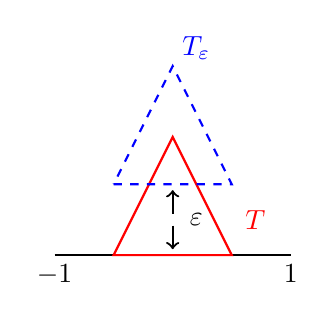
\begin{tikzpicture}[scale=1.5]

		% Draw the real axis segment [-1,1]
		\draw[thick] (-1,0) -- (1,0);
		\draw (-1,0) node[below] {$-1$};
		\draw (1,0) node[below] {$1$};

		% Original triangle T
		\draw[thick, red] (-0.5,0) -- (0.5,0) -- (0,1) -- cycle;
		\node[red] at (.7,.3) {$T$};

		% Shifted triangle T_eps
		\draw[thick, blue, dashed] (-0.5,0.6) -- (0.5,0.6) -- (0,1.6) -- cycle;
		\node[blue] at (.2,1.75) {$T_\varepsilon$};

		% Vertical arrows showing displacement epsilon
		\draw[->, thick] (0,0.35) -- (0,0.55);
		\draw[->, thick] (0,0.25) -- (0,0.05);
		\node at (0.2,0.3) {$\varepsilon$};
	\end{tikzpicture}
	\caption{\small
		The triangle $T$ touches the segment $[-1,1]$ on the real axis.
		Shifting it vertically by $\varepsilon>0$ produces the translated triangle
		$T_\varepsilon = T + i\varepsilon$, which lies entirely in $\mathbb{C}\setminus[-1,1]$.
	}
	\label{fig:tpath}
\end{figure}


\begin{proof}[Solution]
	We assume $f:\mathbb{C}\to\mathbb{C}$ is continuous on $\mathbb{C}$ and analytic on
	$\mathbb{C}\setminus[-1,1]$.
	By Morera’s theorem, it suffices to prove that
	\[
		\int_T f(z)\,dz = 0
	\]
	for every triangular path $T$ in $\mathbb{C}$.

	\medskip
	\noindent\textbf{Case 1: $T$ and its interior avoid $[-1,1]$.}
	If
	\[
		T \cup \mathrm{Int}(T) \subset \mathbb{C}\setminus[-1,1],
	\]
	then $f$ is analytic in a neighborhood of $T$, and by Cauchy’s theorem,
	\[
		\int_T f(z)\,dz = 0.
	\]

	\medskip
	\noindent\textbf{Case 2: One side of $T$ lies on the segment $[-1,1]$.}

	This is the configuration shown in Figure~\ref{fig:tpath}:
	the base of the triangle lies on $[-1,1]$ while the remaining two sides lie in the upper half–plane.
	Let $T$ denote this triangle.
	For $\varepsilon>0$ define its vertical translate
	\[
		T_\varepsilon = T + i\varepsilon.
	\]
	As illustrated in Figure~\ref{fig:tpath}, when $\varepsilon>0$ is small,
	the entire triangle $T_\varepsilon$ (together with its interior) lies strictly above the real axis and therefore satisfies
	\[
		T_\varepsilon \cup \mathrm{Int}(T_\varepsilon)
		\subset\mathbb{C}\setminus[-1,1].
	\]
	Thus, by Case~1,
	\[
		\int_{T_\varepsilon} f(z)\,dz = 0
		\qquad\text{for all sufficiently small }\varepsilon>0.
	\]

	Let $\gamma:[0,1]\to\mathbb{C}$ parametrize $T$.
	Then
	\[
		\gamma_\varepsilon(t)=\gamma(t)+i\varepsilon
	\]
	parametrizes $T_\varepsilon$, and clearly $\gamma_\varepsilon\to\gamma$
	\emph{uniformly} on $[0,1]$ as $\varepsilon\to 0$.

	Since $f$ is continuous on $\mathbb{C}$, it is uniformly continuous on the compact set
	\[
		K:=\bigcup_{0\le\varepsilon\le\varepsilon_0} T_\varepsilon
	\]
	for some small $\varepsilon_0$.
	Therefore $f(\gamma_\varepsilon(t))$ converges uniformly to $f(\gamma(t))$.
	Hence we may pass the limit inside the integral:
	\[
		\int_T f(z)\,dz
		= \int_0^1 f(\gamma(t))\,\gamma'(t)\,dt
		= \lim_{\varepsilon\to 0}\int_0^1 f(\gamma_\varepsilon(t))\,\gamma_\varepsilon'(t)\,dt
		= \lim_{\varepsilon\to 0} \int_{T_\varepsilon} f(z)\,dz = 0.
	\]

	\medskip
	\noindent\textbf{General case.}

	If $T$ intersects $[-1,1]$ in any other way, we divide $T$ into finitely many smaller triangles by inserting straight segments between the points of intersection with $[-1,1]$. A typical example of such a configuration is illustrated in
	Figure~\ref{fig:spath}.
	Each subtriangle is either of type~1 or type~2.
	Applying the two cases above to each subtriangle and summing the resulting integrals yields
	\[
		\int_T f(z)\,dz = 0.
	\]

	\medskip
	\noindent\textbf{Conclusion.}
	Since $\int_T f\,dz=0$ for every triangular path $T$ and $f$ is continuous on $\mathbb{C}$,
	Morera’s theorem implies that $f$ is analytic on all of $\mathbb{C}$.
	Thus $f$ is entire.
\end{proof}

\begin{figure}[t]
	\centering
	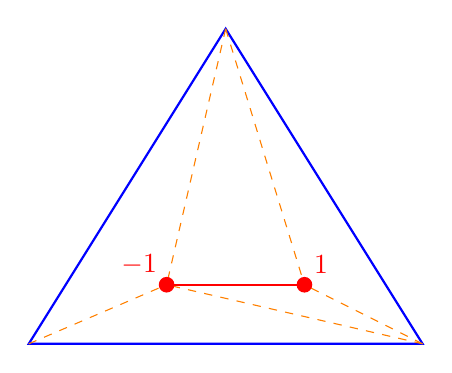
\begin{tikzpicture}[scale=2.5]

		% Coordinates (adjusted to match your sketch)
		\coordinate (d) at (0,1.8);
		\coordinate (e) at (-1,.2);
		\coordinate (c) at (1,0.2);

		\coordinate (b) at (-0.3,0.5);
		\coordinate (a) at (0.4,0.5);

		% Outer triangle (blue)
		\draw[thick, blue] (d) -- (e) -- (c) -- cycle;

		% Subdivision lines (orange)
		\draw[dashed, orange] (d) -- (b);
		\draw[dashed, orange] (d) -- (a);
		\draw[dashed, orange] (e) -- (b);
		\draw[dashed, orange] (c) -- (a);
		\draw[dashed, orange] (c) -- (b);

		% Red connecting segment
		\draw[thick, red] (b) -- (a);

		% Draw points for a, b
		\node[fill=red, circle, inner sep=2pt] at (a) {};
		\node[fill=red, circle, inner sep=2pt] at (b) {};

		% Labels for a, b
		\node[red, right] at (0.4,0.6) {$1$};
		\node[red, left] at (-0.3,0.6) {$-1$};


	\end{tikzpicture}
	\caption{\small
		Subdivision of a triangle by two interior points $1$ and $-1$ and the segment joining them.
	}
	\label{fig:spath}
\end{figure}

\section{The homotopic version of Cauchy's Theorem and simple connectivity}
\setexercise{5}
\begin{exercise}
	Evaluate the integral $\displaystyle \int_{\gamma} \frac{dz}{z^{2}+1}$ where $\gamma(\theta) = 2|\cos 2\theta|\, e^{i\theta}$ for $0 \le \theta \le 2\pi$.
\end{exercise}

\begin{proof}[Solution]
	We are given the curve
	\[
		\gamma(\theta)=2|\cos 2\theta|\,e^{i\theta}, \qquad 0\le \theta\le 2\pi,
	\]
	and we wish to evaluate
	\[
		\int_\gamma \frac{dz}{z^{2}+1}.
	\]

	\textbf{Step 1: Homotope $\gamma$ to the circle $|z|=2$.}
	Define a homotopy
	\[
		H(s,\theta)
		=\big[(1-s)\,2|\cos 2\theta|+2s\big]e^{i\theta},
		\qquad 0\le s\le 1,\ 0\le\theta\le 2\pi.
	\]
	Then $H(0,\theta)=\gamma(\theta)$ and $H(1,\theta)=2e^{i\theta}$.
	We claim $H(s,\theta)\neq \pm i$ for all $(s,\theta)$.
	Indeed, $\pm i$ have modulus $1$, whereas
	\[
		|H(s,\theta)|=(1-s)\,2|\cos 2\theta|+2s\ge 2s\ge 0,
	\]
	and for $\theta=\frac{\pi}{2},\frac{3\pi}{2}$ one has $|H(s,\theta)|=2$.
	Thus $H$ never hits $\pm i$, and therefore gives a homotopy in
	$\mathbb{C}\setminus\{\pm i\}$ from $\gamma$ to the circle
	\[
		\delta(\theta)=2e^{i\theta}.
	\]

	Since $f(z)=\frac{1}{z^{2}+1}$ is analytic on $\mathbb{C}\setminus\{\pm i\}$,
	it follows from homotopy invariance of contour integrals that
	\[
		\int_\gamma \frac{dz}{z^{2}+1}
		=\int_\delta \frac{dz}{z^{2}+1}.
	\]

	\textbf{Step 2: Partial fractions and winding numbers.}
	We write
	\[
		\frac{1}{z^{2}+1}
		=\frac{1}{(z-i)(z+i)}
		=\frac{1}{2i}\left(\frac{1}{z-i}-\frac{1}{z+i}\right).
	\]
	Thus
	\[
		\int_\delta \frac{dz}{z^{2}+1}
		=\frac{1}{2i}
		\left(
		\int_\delta \frac{dz}{z-i}
		-
		\int_\delta \frac{dz}{z+i}
		\right).
	\]

	Now $\delta(\theta)=2e^{i\theta}$ winds once counterclockwise about both
	$i$ and $-i$, since both satisfy $|\,\pm i\,|=1<2$.  Hence
	\[
		n(\delta;i)=1, \qquad n(\delta;-i)=1.
	\]
	By the winding number formula,
	\[
		\int_\delta \frac{dz}{z-i}=2\pi i\cdot n(\delta;i)=2\pi i,
		\qquad
		\int_\delta \frac{dz}{z+i}=2\pi i\cdot n(\delta;-i)=2\pi i.
	\]

	Therefore
	\[
		\int_\delta \frac{dz}{z^{2}+1}
		=\frac{1}{2i}(2\pi i-2\pi i)=0.
	\]

	Hence
	\[
		\int_\gamma \frac{dz}{z^{2}+1}=0.
	\]
\end{proof}


\setexercise{6}
\begin{exercise}
	Let $\gamma(\theta) = \theta e^{i\theta}$ for $0 \le \theta \le 2\pi$ and $\gamma(\theta)= 4\pi - \theta$ for $2\pi \le \theta \le 4\pi$.
	Evaluate $\displaystyle \int_{\gamma} \frac{dz}{z^{2} + \pi^{2}}$.
\end{exercise}

\begin{figure}[h]
	\centering
	\begin{tikzpicture}[scale=0.5]
		% axes
		\draw[->] (-1,0) -- (9,0) node[right] {$\Re z$};
		\draw[->] (0,-7) -- (0,7) node[above] {$\Im z$};

		% mark i pi and -i pi
		\fill (0,3.1416) circle (2pt) node[above right] {$i\pi$};
		\fill (0,-3.1416) circle (2pt) node[below right] {$-i\pi$};

		% spiral: z = theta e^{i\theta}, 0 <= theta <= 2 pi
		\draw[thick, blue, domain=0:6.283, samples=300, variable=\t,
			postaction={decorate},
			decoration={markings, mark=at position 0.25 with {\arrow{>}},
					mark=at position 0.55 with {\arrow{>}},
					mark=at position 0.85 with {\arrow{>}}}]
		plot ({\t*cos(\t r)}, {\t*sin(\t r)});

		% straight return from 2pi to 0
		\draw[thick, blue, postaction={decorate},
			decoration={markings, mark=at position 0.5 with {\arrow{>}}}]
		(6.283,0) -- (0,0);

		% mark 0 and 2 pi
		\fill (0,0) circle (2pt) node[below left] {$0$};
		\fill (6.283,0) circle (2pt) node[below] {$2\pi$};

		% annotations
		\node[blue] at (4,2.5) {$\gamma(\theta)=\theta e^{i\theta}$};
		\node[blue] at (3,-1) {$\gamma(\theta)=4\pi-\theta$};
	\end{tikzpicture}
	\caption{The path $\gamma$: a spiral from $0$ to $2\pi$ followed by a straight line back to $0$.
		The spiral encloses the point $-i\pi$ but not $i\pi$.}
	\label{fig:path}
\end{figure}

\begin{proof}[Solution]
	The curve $\gamma$ is defined by
	\[
		\gamma(\theta)=
		\begin{cases}
			\theta e^{i\theta}, & 0\le \theta \le 2\pi,     \\[4pt]
			4\pi-\theta,        & 2\pi \le \theta \le 4\pi.
		\end{cases}
	\]
	For $0\le\theta\le 2\pi$ the point $\theta e^{i\theta}$ traces a spiral beginning at $0$,
	making one full revolution around the origin, and reaching the point $2\pi$ on the real axis.
	For $2\pi\le\theta\le 4\pi$ the path travels along the real axis from $2\pi$ back to $0$.
	The resulting curve is shown in Figure~\ref{fig:path}.

	\medskip
	The curve winds once counterclockwise
	around the point $-i\pi$, which lies inside the spiral,
	and does not wind around the point $i\pi$, which lies outside the spiral.
	Thus the winding numbers are
	\[
		n(\gamma;-i\pi)=1,
		\qquad
		n(\gamma;i\pi)=0.
	\]

	We compute the integral
	\[
		\int_\gamma \frac{dz}{z^{2}+\pi^{2}}.
	\]
	Using the partial fraction decomposition
	\[
		\frac{1}{z^{2}+\pi^{2}}
		=\frac{1}{(z-i\pi)(z+i\pi)}
		=\frac{1}{2\pi i} \left( \frac{1}{z-i\pi} - \frac{1}{z+i\pi} \right),
	\]
	we obtain
	\[
		\int_\gamma \frac{dz}{z^{2}+\pi^{2}}
		=
		\frac{1}{2\pi i}
		\left(
		\int_\gamma \frac{dz}{z-i\pi}
		-
		\int_\gamma \frac{dz}{z+i\pi}
		\right).
	\]

	By the winding number formula,
	\[
		\int_\gamma \frac{dz}{z-a}
		=
		2\pi i\, n(\gamma;a),
	\]
	so using the winding numbers read off from Figure~\ref{fig:path},
	\[
		\int_\gamma \frac{dz}{z-i\pi}
		=2\pi i\,n(\gamma;i\pi)=0,
		\qquad
		\int_\gamma \frac{dz}{z+i\pi}
		=2\pi i\,n(\gamma;-i\pi)=2\pi i.
	\]

	Substituting these into the previous expression gives
	\[
		\int_\gamma \frac{dz}{z^{2}+\pi^{2}}
		=
		\frac{1}{2\pi i}(0-2\pi i)
		= -1.
	\]
\end{proof}


\setexercise{7}
\begin{exercise}
	Let
	\(
	f(z) = \big[(z - \tfrac{1}{2} - i)(z - 1 - \tfrac{3}{2}i)(z - 1 - i)(z - \tfrac{3}{2} - i)\big]^{-1}
	\)
	and let $\gamma$ be the polygon $[0,\, 2,\, 2+2i,\, 2i,\, 0]$.
	Find $\displaystyle \int_{\gamma} f$.
\end{exercise}

\begin{proof}[Solution]
	Let
	\[
		f(z)=\frac{1}{
			(z-z_1)(z-z_2)(z-z_3)(z-z_4)},
	\]
	where
	\[
		z_1=\tfrac12+i,\qquad
		z_2=1+\tfrac32 i,\qquad
		z_3=1+i,\qquad
		z_4=\tfrac32+i.
	\]
	These are four distinct points, so the partial fraction expansion has the form
	\[
		f(z)=
		\sum_{k=1}^4
		\frac{A_k}{z-z_k},
	\]
	where
	\[
		A_k=\frac{1}{
			\displaystyle \prod_{j\ne k}(z_k-z_j)}.
	\]

	Thus
	\[
		\int_\gamma f(z)\,dz
		=\sum_{k=1}^4 A_k
		\int_\gamma \frac{dz}{z-z_k}.
	\]

	The path
	\[
		\gamma=[0,\,2,\,2+2i,\,2i,\,0]
	\]
	is the positively oriented boundary of the square
	\[
		0<\Re z<2,\qquad 0<\Im z<2.
	\]
	A simple check of real and imaginary parts shows that all four points
	\(z_1,z_2,z_3,z_4\) lie inside this square.
	Therefore
	\[
		n(\gamma;z_k)=1
		\qquad\text{for }k=1,2,3,4,
	\]
	and hence
	\[
		\int_\gamma \frac{dz}{z-z_k}
		=2\pi i.
	\]

	Therefore
	\[
		\int_\gamma f(z)\,dz
		=\sum_{k=1}^4 A_k \cdot 2\pi i
		=
		2\pi i \sum_{k=1}^4 A_k.
	\]

	It remains to compute the four coefficients \(A_k\).  A direct computation gives
	\[
		A_1=-2+2i,\qquad
		A_2=-4i,\qquad
		A_3=-8i,\qquad
		A_4=2+2i.
	\]

	Adding them,
	\[
		A_1+A_2+A_3+A_4
		=(-2+2)+(2i-4i-8i+2i)
		=-8i.
	\]

	Thus
	\[
		\int_\gamma f(z)\,dz
		=2\pi i\,(-8i)
		=16\pi.
	\]
\end{proof}


\setexercise{10}
\begin{exercise}
	Find all possible values of $\displaystyle \int_{\gamma} \frac{dz}{1 + z^{2}}$ where $\gamma$ is any closed rectifiable curve.
\end{exercise}

\begin{proof}[Solution]
	We use the partial fraction decomposition
	\[
		\frac{1}{1+z^{2}}
		=\frac{1}{(z-i)(z+i)}
		=\frac{1}{2i}\left(\frac{1}{z-i}-\frac{1}{z+i}\right).
	\]
	For any closed rectifiable curve $\gamma$ and any $a\in\mathbb{C}$, we have
	\[
		\int_\gamma \frac{dz}{z-a}
		= 2\pi i\, n(\gamma;a),
	\]
	where $n(\gamma;a)$ is the winding number of $\gamma$ about $a$.
	Therefore
	\[
		\int_\gamma \frac{dz}{1+z^{2}}
		=\frac{1}{2i}
		\left(2\pi i\, n(\gamma;i) - 2\pi i\, n(\gamma;-i)\right)
		=\pi\bigl(n(\gamma;i)-n(\gamma;-i)\bigr).
	\]

	Since $n(\gamma;i)$ and $n(\gamma;-i)$ may be any integers (positive, negative, or zero)
	depending on how the curve winds around $i$ and $-i$, the integral may take any value of the form
	\[
		\{\pi k : k\in\mathbb{Z}\}.
	\]
\end{proof}
\section{Counting zeros; the Open Mapping Theorem}
\setexercise{4}
\begin{exercise}
	Suppose that $f : G \to \mathbb{C}$ is analytic and one--one; show that $f'(z) \neq 0$ for any $z$ in $G$.
\end{exercise}

\begin{proof}[Solution]
	Let $f : G \to \mathbb{C}$ be analytic and one--one, and fix a point
	$a \in G$.  We show that $f'(a) \neq 0$.
	Suppose for contradiction that $f'(a)=0$.
	Then $f(z)-f(a)$ has a zero at $z=a$ of multiplicity $m \ge 2$.
	By Theorem~7.4, there exist $\varepsilon>0$ and $\delta>0$ such that
	whenever $0<|\zeta - f(a)| < \delta$, the equation
	\[
		f(z)=\zeta
	\]
	has \emph{exactly $m$ distinct solutions} in the disk $B(a;\varepsilon)$.
	Since $m\ge 2$, every $\zeta$ sufficiently close to $f(a)$ is taken at
	least twice by $f$.
	This contradicts the assumption that $f$ is one--one on~$G$.
	Therefore our assumption was impossible, and we must have $f'(a) \neq 0$.
	As $a$ was arbitrary, it follows that
	\[
		f'(z) \neq 0 \qquad \text{for all } z \in G.
	\]
\end{proof}

\chapter{Singularity}
\section{Classification of singularities}
\setexercise{4}
\begin{exercise}
	Let
	\[
		f(z)=\frac{1}{z(z-1)(z-2)};
	\]
	give the Laurent expansion of \(f(z)\) in each of the following annuli:
	(a) ann\((0;0,1)\);
	(b) ann\((0;1,2)\);
	(c) ann\((0;2,\infty)\).
\end{exercise}

\begin{proof}[Solution]
	We start from the partial fraction decomposition
	\[
		f(z)=\frac{1}{z(z-1)(z-2)}
		= \frac{1}{2z}-\frac{1}{z-1}+\frac{1}{2(z-2)}.
	\]

	We expand in powers of $z$ using geometric series formula.

	%--------------------------------------------------
	\textbf{(a) The annulus } $0<|z|<1$.

	\[
		\frac{1}{z-1}
		= -\sum_{n=0}^{\infty} z^n,
		\qquad
		\frac{1}{z-2}
		= -\frac12 \sum_{n=0}^{\infty} \left(\frac{z}{2}\right)^n.
	\]
	Thus
	\[
		f(z)=\frac12 z^{-1}
		+ \sum_{n=0}^{\infty} z^n
		- \frac14 \sum_{n=0}^{\infty} 2^{-n} z^n.
	\]

	Therefore the Laurent coefficients are
	\[
		a_{-1}=\frac12,\qquad
		a_n = 1 - 2^{-(n+2)} \ (n\ge 0),\qquad
		a_n=0\ (n\le -2).
	\]
	So
	\[
		f(z)=\frac12 z^{-1}
		+ \sum_{n=0}^{\infty} \left(1-2^{-(n+2)}\right) z^{n},
		\qquad 0<|z|<1.
	\]

	%--------------------------------------------------

	\textbf{(b) The annulus } $1 < |z| < 2$.

	\[
		\frac{1}{z-1}
		= \frac{1}{z} \frac{1}{1-\frac{1}{z}}
		= \sum_{n=1}^{\infty} z^{-n},
		\qquad
		\frac{1}{z-2}
		= -\frac12 \frac{1}{1-\frac{z}{2}}
		= -\frac12 \sum_{n=0}^{\infty} \left(\frac{z}{2}\right)^n.
	\]
	Hence
	\[
		f(z)
		= \frac12 z^{-1}
		- \sum_{n=1}^{\infty} z^{-n}
		- \frac14 \sum_{n=0}^{\infty} 2^{-n} z^{\,n}.
	\]

	The coefficients are

	\[
		a_{-1}= -\frac12,
		\qquad
		a_{-n} = -1 \quad (n \ge 2),
		\qquad
		a_n = -2^{-(n+2)} \quad (n \ge 0).
	\]
	Thus,
	\[
		f(z)
		= -\frac12 z^{-1}
		- \sum_{n=2}^{\infty} z^{-n}
		- \sum_{n=0}^{\infty} 2^{-(n+2)}z^{\,n},
		\qquad 1<|z|<2.
	\]

	%--------------------------------------------------
	\textbf{(c) The annulus } $|z|>2$.

	To apply the geometric series here, we factor out $z$ so that $|1/z|$ and $|2/z|$ are less than $1$ in the annuli.


	\[
		\frac{1}{z-1} = \frac{1}{z} \frac{1}{1-\frac{1}{z}}
		= \sum_{n=1}^{\infty} z^{-n},
		\qquad
		\frac{1}{z-2}= \frac{1}{z} \frac{1}{1-\frac{2}{z}}
		= \sum_{n=1}^{\infty} \frac{2^{n-1}}{z^{n}}.
	\]
	Hence
	\[
		f(z)=\frac12 z^{-1}
		-\sum_{n=1}^{\infty} z^{-n}
		+ \sum_{n=1}^{\infty} 2^{\,n-2} z^{-n}.
	\]

	The coefficients are
	\[
		a_{-1}=0,
		\qquad
		a_{-n}=2^{\,n-2}-1 \ (n\ge 2),
		\qquad
		a_n=0 \ (n\ge 0).
	\]
	Thus
	\[
		f(z)=\sum_{n=2}^{\infty} \left(2^{\,n-2}-1\right) z^{-n},
		\qquad |z|>2.
	\]
\end{proof}

\setexercise{15}
\begin{exercise}
	Let \( f \) be analytic in
	\[
		G = \{ z : 0 < |z - a| < r \}
	\]
	except that there is a sequence of poles \( \{a_n\} \) in \(G\) with \(a_n \to a\).
	Show that for any \( \omega \in \mathbb{C} \) there exists a sequence \( \{z_n\} \subset G \) with
	\[
		a = \lim z_n \quad \text{and} \quad \omega = \lim f(z_n).
	\]
\end{exercise}


\begin{proof}[Solution]
	Fix \(\omega \in \mathbb C\). We show that \(\omega\) is a cluster value of
	\(f\) at \(a\).

	Suppose not. Then there exist \(\varepsilon>0\) and \(0<\rho<r\) such that
	\[
		|f(z)-\omega|\ge \varepsilon
	\]
	whenever \(0<|z-a|<\rho\) and \(z\) is not a pole of \(f\).

	Define
	\[
		g(z)=\frac{1}{f(z)-\omega}
	\]
	at all points where \(f\) is analytic. Then
	\[
		|g(z)|\le \frac{1}{\varepsilon}.
	\]
	If \(b\) is a pole of \(f\), then \(f-\omega\) also has a pole at \(b\), and
	therefore \(g=1/(f-\omega)\) has a removable singularity at \(b\). Define
	\(g(b)=0\). Thus \(g\) extends to a bounded holomorphic function on
	\[
		0<|z-a|<\rho .
	\]

	Since \(g\) is bounded near \(a\), the removable singularity theorem implies
	that \(g\) extends holomorphically to \(a\). Hence \(g\) is holomorphic on
	\[
		|z-a|<\rho .
	\]

	Now \(a_n\to a\), so for all sufficiently large \(n\), \(a_n\in \{0<|z-a|<\rho\}\).
	At each such pole \(a_n\), by the definition of the removable extension,
	\[
		g(a_n)=0.
	\]
	Thus \(g\) has zeros accumulating at \(a\). Since \(g\) is holomorphic on
	\(|z-a|<\rho\), the identity theorem gives
	\[
		g\equiv 0
	\]
	on \(|z-a|<\rho\). This is impossible, because wherever \(f\) is analytic,
	\[
		g(z)=\frac{1}{f(z)-\omega}
	\]
	cannot be equal to \(0\).

	Therefore our supposition was false. Hence for every \(n\in\mathbb N\), there
	exists \(z_n\in G\), not a pole of \(f\), such that
	\[
		0<|z_n-a|<\frac1n
		\qquad\text{and}\qquad
		|f(z_n)-\omega|<\frac1n.
	\]
	It follows that
	\[
		z_n\to a
		\qquad\text{and}\qquad
		f(z_n)\to \omega .
	\]
	Since \(\omega\in\mathbb C\) was arbitrary, the result follows.
\end{proof}
\section{Residues}

\setexercise{2}
\begin{exercise}[c]
	Verify the following equation:
	\[
		\int_{0}^{\infty} \frac{\cos(ax)}{(1+x^{2})^{2}}\, dx
		= \frac{\pi (a+1)e^{-a}}{4}, \qquad a>0.
	\]
\end{exercise}

\begin{proof}[Solution]
	We want to show that for $a>0$,
	\[
		\int_{0}^{\infty} \frac{\cos(ax)}{(1+x^{2})^{2}}\, dx
		= \frac{\pi (a+1)e^{-a}}{4}.
	\]

	Consider the complex-valued function
	\[
		f(z) = \frac{e^{iaz}}{(1+z^{2})^{2}}, \qquad a>0,
	\]
	and for  \(R>1\) integrate it over the semicircular contour $C_R$ in the upper half–plane,
	consisting of the segment $[-R,R]$ on the real axis and the semicircle
	\[
		\gamma_R : z = Re^{it}, \quad t \in [0,\pi].
	\]

	The singularities of $f$ are at $z = i$ and $z = -i$. In the upper half–plane
	only $z = i$ lies inside the contour, and it is a pole of order two.
	By the residue theorem,
	\[
		\int_{C_R} f(z)\,dz = 2\pi i\,Res(f;i).
	\]

	\medskip

	\noindent\textbf{The integral over the semicircle.}
	We claim that
	\[
		\int_{\gamma_R} f(z)\,dz \longrightarrow 0 \quad \text{as } R\to\infty.
	\]
	On $\gamma_R$ we have $z = Re^{it}$, $t\in[0,\pi]$, hence
	\[
		|e^{iaz}| = \bigl|e^{iaRe^{it}}\bigr|
		= e^{\Re(i a R e^{it})}
		= e^{-aR\sin t} \le 1.
	\]
	Moreover, for $R>1$,
	\[
		|1+z^2|
		= |1+R^2 e^{2it}|
		\ge \bigl||z|^{2}-1\bigr| = R^2 - 1,
	\]
	so
	\[
		|(1+z^2)^2| \ge (R^2 - 1)^2.
	\]
	Therefore, for $R>1$,
	\[
		\sup_{z\in\gamma_R} |f(z)|
		\le \frac{1}{(R^2-1)^2}.
	\]
	The length of $\gamma_R$ is $\pi R$, so
	\[
		\left|\int_{\gamma_R} f(z)\,dz\right|
		\le \text{(length of $\gamma_R$)}\cdot \sup_{z\in\gamma_R}|f(z)|
		\le \pi R \cdot \frac{1}{(R^2-1)^2}
		\longrightarrow 0 \quad\text{as } R\to\infty.
	\]
	Thus
	\[
		\int_{-\infty}^{\infty} \frac{e^{iax}}{(1+x^{2})^{2}}\,dx
		= 2\pi i\,Res(f;i).
	\]

	\medskip

	\noindent\textbf{Residue at $z=i$.}
	We write
	\[
		f(z) = \frac{e^{iaz}}{(z^2+1)^2}
		= \frac{e^{iaz}}{(z-i)^2(z+i)^2}.
	\]
	Thus $z=i$ is a double pole. For a double pole at $z=i$ we have
	\[
		Res(f;i)
		= \left.\frac{d}{dz}\bigl[(z-i)^2 f(z)\bigr]\right|_{z=i}
		= \left.\frac{d}{dz}\left(\frac{e^{iaz}}{(z+i)^2}\right)\right|_{z=i}.
	\]
	Set
	\[
		g(z) = \frac{e^{iaz}}{(z+i)^2}.
	\]
	Then
	\[
		g'(z)
		= \frac{e^{iaz}\big(ia(z+i)^2 - 2(z+i)\big)}{(z+i)^4}.
	\]
	So
	\begin{align*}
		g'(i)
		 & = \frac{e^{iai}\big(ia(-4) - 2(2i)\big)}{16}
		= -\frac{i}{4}(a+1)e^{-a}.
	\end{align*}
	Hence
	\[
		Res(f;i) = -\frac{i}{4}(a+1)e^{-a}.
	\]

	Thus
	\[
		\int_{-\infty}^{\infty} \frac{e^{iax}}{(1+x^{2})^{2}}\,dx
		= 2\pi i\left(-\frac{i}{4}(a+1)e^{-a}\right)
		= \frac{\pi}{2}(a+1)e^{-a}.
	\]

	\medskip

	\noindent\textbf{Extracting the cosine integral.}
	Write
	\[
		\int_{-\infty}^{\infty} \frac{e^{iax}}{(1+x^{2})^{2}}\,dx
		= \int_{-\infty}^{\infty} \frac{\cos(ax)}{(1+x^{2})^{2}}\,dx
		+ i\int_{-\infty}^{\infty} \frac{\sin(ax)}{(1+x^{2})^{2}}\,dx.
	\]
	The integrand of the sine term is odd, so
	\[
		\int_{-\infty}^{\infty} \frac{\sin(ax)}{(1+x^{2})^{2}}\,dx = 0.
	\]
	The integrand of the cosine term is even, hence
	\[
		\int_{-\infty}^{\infty} \frac{\cos(ax)}{(1+x^{2})^{2}}\,dx
		= 2\int_{0}^{\infty} \frac{\cos(ax)}{(1+x^{2})^{2}}\,dx.
	\]
	Therefore,
	\[
		2\int_{0}^{\infty} \frac{\cos(ax)}{(1+x^{2})^{2}}\,dx
		= \frac{\pi}{2}(a+1)e^{-a},
	\]
	which implies
	\[
		\int_{0}^{\infty} \frac{\cos(ax)}{(1+x^{2})^{2}}\,dx
		= \frac{\pi}{4}(a+1)e^{-a},
	\]
	as required.
\end{proof}

\section{The Argument Principle}
\setexercise{2}
\begin{exercise}
	Suppose \( f \) is analytic on \( \overline{B(0;1)} \) and satisfies
	\( |f(z)| < 1 \) for \( |z| = 1 \).
	Find the number of solutions (counting multiplicities) of the equation
	\[
		f(z) = z^{n}
	\]
	where \( n \) is an integer larger than or equal to \( 1 \).
\end{exercise}

\begin{proof}[Solution]
	We seek the number of solutions of
	\[
		f(z) = z^{n} \qquad (n \ge 1).
	\]
	Rewrite this as
	\[
		f(z) - z^{n} = 0.
	\]

	Define
	\[
		h(z) = z^{n}, \qquad g(z) = f(z) - z^{n}.
	\]
	Both $g$ and $h$ are analytic on and inside the unit circle
	$\gamma = \{z : |z| = 1\}$.

	On $\gamma$ we have $|h(z)| = |z^{n}| = 1$, and by hypothesis
	\[
		|h(z) + g(z)| = |f(z)| < 1 = |h(z)|.
	\]
	Thus the inequality required by Rouché’s theorem holds on $\gamma$.
	Therefore $h$ and $g$ have the same number of zeros inside $\gamma$.
	Since $h(z) = z^{n}$ has exactly $n$ zeros in $|z| < 1$,
	it follows that $g(z) = f(z) - z^{n}$ has exactly $n$ zeros in $|z| < 1$.
	Thus the equation $f(z) = z^{n}$ has exactly $n$ solutions in the unit disk.
\end{proof}

\chapter{The Maximum Modulus Theorem}
\section{The Maximum Principle}
\setexercise{2}
\begin{exercise}
	Let $G$ be a bounded region and suppose $f$ is continuous on $\overline{G}$ and analytic on $G$. Show that if there is a constant $c \ge 0$ such that $|f(z)| = c$ for all $z$ on the boundary of $G$, then either $f$ is a constant function or $f$ has a zero in $G$.
\end{exercise}
\begin{proof}[Solution]
	Let $G$ be a bounded region, and let $f$ be continuous on $\overline{G}$ and analytic on $G$. Assume that
	\[
		|f(z)| = c \quad \text{for all } z \in \partial G,
	\]
	where $c \ge 0$.

	\medskip
	\noindent
	\textbf{Case 1: $c=0$.}
	Then $f=0$ on $\partial G$. By the maximum modulus principle,
	\[
		\max_{\overline{G}} |f| = \max_{\partial G} |f| = 0,
	\]
	so $f \equiv 0$ on $G$, hence $f$ is constant.

	\medskip
	\noindent
	\textbf{Case 2: $c>0$.}
	Suppose that $f$ has no zeros in $G$. Then $|f|$ is a positive continuous function on $\overline{G}$ and is the modulus of a nonvanishing analytic function on $G$. Hence, by the minimum modulus principle,
	\[
		\min_{\overline{G}} |f| = \min_{\partial G} |f|.
	\]
	Since $|f|=c$ on $\partial G$, we get
	\[
		\min_{\overline{G}} |f| = c,
	\]
	and therefore \(|f(z)| \ge c\) for all \(z\in G\).

	On the other hand, by the maximum modulus principle applied to $f$,
	\[
		\max_{\overline{G}} |f| = \max_{\partial G} |f| = c,
	\]
	so \(|f(z)| \le c\) for all \(z\in G\).

	Combining the two inequalities yields \(|f(z)|=c\) for all \(z\in G\). By the maximum modulus principle (in its strong form), an analytic function whose modulus is constant on a region must be constant. Hence $f$ is constant.

	\medskip
	\noindent
	Therefore, either $f$ is constant or $f$ has a zero in $G$.
\end{proof}



\setexercise{6}
\begin{exercise}
	Suppose that both $f$ and $g$ are analytic on $\overline{B(0;R)}$ with
	\[
		|f(z)| = |g(z)| \quad \text{for } |z| = R.
	\]
	Show that if neither $f$ nor $g$ vanishes in $B(0;R)$, then there is a constant $\lambda$, with $|\lambda| = 1$, such that $f = \lambda g$.
\end{exercise}

\begin{proof}[Solution]
	Assume $f$ and $g$ are analytic on $\overline{B(0;R)}$ and satisfy $|f(z)|=|g(z)|$ for $|z|=R$. Also assume neither $f$ nor $g$ vanishes in $B(0;R)$.

	Since $g$ has no zeros in $B(0;R)$, the quotient
	\[
		h(z):=\frac{f(z)}{g(z)}
	\]
	is analytic on $B(0;R)$. On the boundary $|z|=R$ we have
	\[
		|h(z)|=\frac{|f(z)|}{|g(z)|}=1.
	\]
	Because $h$ is continuous on $\overline{B(0;R)}$ and $|h|$ attains both its maximum and minimum on the boundary, the maximum modulus principle gives
	\[
		|h(z)|\le 1 \quad \text{for } |z|<R,
	\]
	and since $h$ is nonvanishing (as $f$ is also nonvanishing in $B(0;R)$), the minimum modulus principle gives
	\[
		|h(z)|\ge 1 \quad \text{for } |z|<R.
	\]
	Hence $|h(z)|\equiv 1$ throughout $B(0;R)$.

	An analytic function with constant modulus on a region must be constant. Therefore $h$ is constant, say $h\equiv \lambda$, and then $|\lambda|=1$ (because $|h|=1$). Thus
	\[
		f=\lambda g \quad \text{on } B(0;R),
	\]
	and by continuity the same holds on $\overline{B(0;R)}$.
\end{proof}


\setexercise{7}
\begin{exercise}
	Let $f$ be analytic in the disk $B(0;R)$ and for $0 \le r < R$ define
	\[
		A(r) = \max \{ \Re f(z) : |z| = r \}.
	\]
	Show that unless $f$ is a constant, $A(r)$ is a strictly increasing function of $r$.
\end{exercise}

\begin{proof}[Solution]
	Define
	\[
		g(z)=e^{f(z)}.
	\]
	Since $f$ is analytic in $B(0;R)$, the function $g$ is also analytic there. Moreover,
	\[
		|g(z)|=|e^{f(z)}|=e^{\Re f(z)}.
	\]
	Hence for each $0\le r<R$,
	\[
		\max_{|z|=r}|g(z)|
		=\max_{|z|=r} e^{\Re f(z)}
		= e^{\max_{|z|=r}\Re f(z)}
		= e^{A(r)}.
	\]

	Now let
	\[
		M(r)=\max_{|z|=r}|g(z)|.
	\]
	By the maximum modulus principle, \(M(r)\) is an increasing function of \(r\). Therefore \(e^{A(r)}\) is increasing, and since the exponential function is strictly increasing on \(\mathbb R\), it follows that \(A(r)\) is increasing.

	It remains to prove strict increase unless \(f\) is constant. Suppose there exist \(0\le r_1<r_2<R\) such that
	\[
		A(r_1)=A(r_2).
	\]
	Then
	\[
		M(r_1)=e^{A(r_1)}=e^{A(r_2)}=M(r_2).
	\]
	So the maximum modulus of the analytic function \(g\) is the same on the circles \(|z|=r_1\) and \(|z|=r_2\). Since \(r_1<r_2\), the maximum modulus principle implies that \(g\) must be constant on \(B(0;r_2)\). Thus \(e^{f(z)}\) is constant, say
	\[
		e^{f(z)}=c \neq 0.
	\]
	Differentiating, we get
	\[
		f'(z)e^{f(z)}=0.
	\]
	Because \(e^{f(z)}\neq 0\), it follows that
	\[
		f'(z)=0
	\]
	for all \(z\in B(0;r_2)\). Hence \(f\) is constant on \(B(0;r_2)\), and therefore constant on \(B(0;R)\).

	Thus, unless \(f\) is constant, equality \(A(r_1)=A(r_2)\) cannot happen when \(r_1<r_2\). Therefore
	\[
		A(r_1)<A(r_2)\qquad\text{whenever }0\le r_1<r_2<R.
	\]
	So \(A(r)\) is strictly increasing unless \(f\) is constant.
\end{proof}

\section{Schwarz's Lemma}
\setexercise{1}
\begin{exercise}
	Suppose $|f(z)| \le 1$ for $|z|<1$ and $f$ is a non-constant analytic function.
	By considering the function $g : \mathbb{D} \to \mathbb{D}$ defined by
	\[
		g(z) = \frac{f(z)-a}{1-\overline{a}\,f(z)}
	\]
	where $a = f(0)$, prove that
	\[
		\frac{|f(0)|-|z|}{1+|f(0)|\,|z|}
		\le |f(z)| \le
		\frac{|f(0)|+|z|}{1-|f(0)|\,|z|}
	\]
	for $|z|<1$.
\end{exercise}

\begin{proof}[Solution]
	Let $a=f(0)$ and define
	\[
		g(z)=\frac{f(z)-a}{1-\overline{a}\,f(z)}.
	\]
	Since $|f(z)|\le 1$ for $|z|<1$ and $|a|<1$, the map
	\[
		w \mapsto \frac{w-a}{1-\overline{a}\,w}
	\]
	is an automorphism of the unit disk $\mathbb{D}$. Hence $g:\mathbb{D}\to\mathbb{D}$ is analytic. Moreover,
	\[
		g(0)=\frac{f(0)-a}{1-\overline{a}f(0)}=0.
	\]

	Because $f$ is non-constant, $g$ is also non-constant. Therefore by Schwarz's lemma,
	\[
		|g(z)|\le |z| \qquad \text{for } |z|<1.
	\]
	Thus
	\[
		\left|\frac{f(z)-a}{1-\overline{a}\,f(z)}\right|\le |z|.
	\]
	Let $w=f(z)$. Then
	\[
		|w-a|\le |z|\,|1-\overline{a}\,w|.
	\]

	\textbf{Upper bound.}
	Using the triangle inequality,
	\[
		|w-a|\ge ||w|-|a|| \ge |w|-|a|
	\]
	and
	\[
		|1-\overline{a}\,w|\le 1+|a|\,|w|.
	\]
	Hence
	\[
		|w|-|a|\le |z|(1+|a|\,|w|).
	\]
	Rearranging gives
	\[
		|w|(1-|a||z|)\le |a|+|z|,
	\]
	so
	\[
		|f(z)|=|w|\le \frac{|a|+|z|}{1-|a||z|}.
	\]

	\textbf{Lower bound.}
	Again from
	\[
		|w-a|\le |z|\,|1-\overline{a}\,w|,
	\]
	we use
	\[
		|w-a|\ge |a|-|w|
	\]
	and
	\[
		|1-\overline{a}\,w|\le 1+|a|\,|w|.
	\]
	Thus
	\[
		|a|-|w|\le |z|(1+|a|\,|w|).
	\]
	Rearranging yields
	\[
		|a|-|z|\le |w|(1+|a||z|),
	\]
	and therefore
	\[
		|f(z)|=|w|\ge \frac{|a|-|z|}{1+|a||z|}.
	\]

	Since $a=f(0)$, we conclude that for $|z|<1$,
	\[
		\frac{|f(0)|-|z|}{1+|f(0)|\,|z|}
		\le |f(z)| \le
		\frac{|f(0)|+|z|}{1-|f(0)|\,|z|}.
	\]
\end{proof}

\setexercise{3}
\begin{exercise}
	Suppose $f:\mathbb{D}\to\mathbb{C}$ satisfies $\Re f(z)\ge 0$ for all $z\in\mathbb{D}$ and suppose that $f$ is analytic and not constant.
	\begin{enumerate}[label=(\alph*)]
		\item Show that $\Re f(z)>0$ for all $z\in\mathbb{D}$.
		\item By using an appropriate M\"obius transformation, apply Schwarz's Lemma to prove that if $f(0)=1$ then
		      \[
			      |f(z)| \le \frac{1+|z|}{1-|z|}
		      \]
		      for $|z|<1$. What can be said if $f(0)\ne 1$?
		\item Show that if $f(0)=1$, $f$ also satisfies
		      \[
			      |f(z)| \ge \frac{1-|z|}{1+|z|}.
		      \]
		      Hint: Use part (a).
	\end{enumerate}
\end{exercise}

\begin{proof}[Solution]
	\begin{enumerate}[label=(\alph*)]
		\item Let
		      \[
			      u(z)=\Re f(z).
		      \]
		      Since \(f\) is analytic on \(\mathbb D\), the function \(u\) is harmonic on \(\mathbb D\). We are given that
		      \[
			      u(z)\ge 0 \qquad (z\in\mathbb D).
		      \]
		      Suppose there exists \(z_0\in\mathbb D\) such that \(u(z_0)=0\). Then \(u\) attains its minimum value at an interior point. By the minimum principle for harmonic functions, \(u\) must be constant on \(\mathbb D\). Hence \(\Re f\) is constant.

		      If \(f=u+iv\) and \(u\) is constant, then \(u_x=u_y=0\). By the Cauchy--Riemann equations,
		      \[
			      v_x=-u_y=0,\qquad v_y=u_x=0,
		      \]
		      so \(v\) is also constant. Therefore \(f\) is constant, contrary to hypothesis. Hence no such \(z_0\) exists, and so
		      \[
			      \Re f(z)>0 \qquad \text{for all } z\in\mathbb D.
		      \]

		\item Assume \(f(0)=1\). Since \(\Re f(z)>0\) for all \(z\in\mathbb D\), the image of \(f\) lies in the right half-plane. Consider the M\"obius transformation
		      \[
			      \phi(w)=\frac{w-1}{w+1}.
		      \]
		      This maps the right half-plane \(\{w:\Re w>0\}\) into \(\mathbb D\). Define
		      \[
			      g(z)=\phi(f(z))=\frac{f(z)-1}{f(z)+1}.
		      \]
		      Then \(g:\mathbb D\to\mathbb D\) is analytic, and
		      \[
			      g(0)=\frac{f(0)-1}{f(0)+1}=0.
		      \]
		      By Schwarz's Lemma,
		      \[
			      |g(z)|\le |z| \qquad (z\in\mathbb D).
		      \]
		      Thus
		      \[
			      \left|\frac{f(z)-1}{f(z)+1}\right|\le |z|.
		      \]

		      Let \(r=|z|\) and write \(w=f(z)\). Then
		      \[
			      |w-1|\le r\,|w+1|.
		      \]
		      Using the triangle inequality,
		      \[
			      |w|-1\le |w-1|\le r\,|w+1|\le r(|w|+1).
		      \]
		      Hence
		      \[
			      |w|-1\le r|w|+r,
		      \]
		      so
		      \[
			      |w|(1-r)\le 1+r.
		      \]
		      Therefore
		      \[
			      |f(z)|\le \frac{1+|z|}{1-|z|}.
		      \]

		      If \(f(0)\ne 1\), let \(a=f(0)\), so \(\Re a>0\). Then
		      \[
			      \psi(w)=\frac{w-a}{w+\overline a}
		      \]
		      maps the right half-plane into \(\mathbb D\), and \(\psi(a)=0\). Thus
		      \[
			      h(z)=\psi(f(z))=\frac{f(z)-a}{f(z)+\overline a}
		      \]
		      is analytic from \(\mathbb D\) to \(\mathbb D\) with \(h(0)=0\). By Schwarz's Lemma,
		      \[
			      \left|\frac{f(z)-a}{f(z)+\overline a}\right|\le |z|.
		      \]
		      This gives the corresponding estimate for general \(f(0)=a\):
		      \[
			      |f(z)|\le \frac{|a|(1+|z|)}{1-|z|}.
		      \]

		\item Again assume \(f(0)=1\). From part (a), \(\Re f(z)>0\) for all \(z\in\mathbb D\). Hence
		      \[
			      \Re\!\left(\frac{1}{f(z)}\right)
			      = \frac{\Re f(z)}{|f(z)|^2}>0,
		      \]
		      so the function
		      \[
			      F(z)=\frac{1}{f(z)}
		      \]
		      is analytic on \(\mathbb D\), non-constant, and satisfies \(\Re F(z)>0\) for all \(z\in\mathbb D\). Also,
		      \[
			      F(0)=\frac{1}{f(0)}=1.
		      \]
		      Applying part (b) to \(F\), we obtain
		      \[
			      |F(z)|\le \frac{1+|z|}{1-|z|}.
		      \]
		      That is,
		      \[
			      \frac{1}{|f(z)|}\le \frac{1+|z|}{1-|z|}.
		      \]
		      Taking reciprocals gives
		      \[
			      |f(z)|\ge \frac{1-|z|}{1+|z|}.
		      \]

		      This proves all three parts.
	\end{enumerate}
\end{proof}

\setexercise{6}
\begin{exercise}
	Suppose $f$ is analytic in some region containing $\overline{B}(0,1)$ and $|f(z)|=1$ where $|z|=1$.
	Find a formula for $f$. Hint: First consider the case where $f$ has no zeros in $B(0,1)$.
\end{exercise}

\begin{proof}[Solution]
	We shall show that \(f\) must be a finite Blaschke product. That is,
	\[
		f(z)=\lambda \prod_{k=1}^n \frac{z-a_k}{1-\overline{a_k}z},
		\qquad |\lambda|=1,\quad |a_k|<1.
	\]

	Since \(f\) is analytic in a region containing \(\overline{B}(0,1)\), it is analytic on a neighborhood of the closed unit disk. Because
	\[
		|f(z)|=1 \qquad (|z|=1),
	\]
	\(f\) has no zeros on the unit circle.
	Let \(a_1,\dots,a_n\) be the zeros of \(f\) in \(B(0,1)\), counted with multiplicity. Since \(f\) is analytic on a neighborhood of \(\overline{B}(0,1)\), it has only finitely many such zeros.

	\medskip
	\textbf{Case 1: \(f\) has no zeros in \(B(0,1)\).}

	Then \(f\) has no zeros on \(\overline{B}(0,1)\), so \(1/f\) is analytic on a neighborhood of \(\overline{B}(0,1)\).
	Since \(f\) is analytic on the disk and continuous on the boundary, the maximum modulus principle implies
	\[
		|f(z)| \le 1 \qquad (|z|<1).
	\]

	Because \(1/f\) is also analytic and satisfies
	\[
		\left|\frac{1}{f(z)}\right|=1 \qquad (|z|=1),
	\]
	the maximum modulus principle applied to \(1/f\) gives
	\[
		\left|\frac{1}{f(z)}\right| \le 1 \qquad (|z|<1),
	\]
	hence
	\[
		|f(z)| \ge 1.
	\]

	Therefore
	\[
		|f(z)|=1 \qquad (|z|<1).
	\]

	If \(f\) were nonconstant, the open mapping theorem would imply that \(f(B(0,1))\) is open, which is impossible since it lies in the unit circle. Thus \(f\) is constant:
	\[
		f(z)\equiv \lambda, \qquad |\lambda|=1.
	\]

	\medskip
	\textbf{Case 2: general case.}

	Let
	\[
		B(z)=\prod_{k=1}^n \frac{z-a_k}{1-\overline{a_k}z}.
	\]
	This is a finite Blaschke product. Since \(|a_k|<1\), each factor is analytic on a neighborhood of \(\overline{B}(0,1)\). Moreover, for \(|z|=1\),
	\[
		\left|\frac{z-a_k}{1-\overline{a_k}z}\right|=1,
	\]
	so
	\[
		|B(z)|=1 \qquad (|z|=1).
	\]

	Define
	\[
		g(z)=\frac{f(z)}{B(z)}.
	\]
	The zeros of \(B\) in \(B(0,1)\) are exactly \(a_1,\dots,a_n\) with the same multiplicities, so the singularities of \(f/B\) at these points are removable. Hence \(g\) is analytic in \(B(0,1)\), and in fact analytic on a neighborhood of \(\overline{B}(0,1)\).

	Moreover, \(g\) has no zeros in \(B(0,1)\), and for \(|z|=1\),
	\[
		|g(z)|=\frac{|f(z)|}{|B(z)|}=1.
	\]

	Thus \(g\) satisfies the conditions of Case 1, so \(g\) is constant:
	\[
		g(z)\equiv \lambda
		\qquad \text{for some } |\lambda|=1.
	\]

	Therefore
	\[
		f(z)=\lambda B(z)
		=\lambda \prod_{k=1}^n \frac{z-a_k}{1-\overline{a_k}z},
		\qquad |\lambda|=1,\quad |a_k|<1.
	\]

	Hence every analytic function on a neighborhood of \(\overline{B}(0,1)\) satisfying \( |f(z)|=1 \) on \( |z|=1 \) is a finite Blaschke product times a unimodular constant.
\end{proof}

\section{Convex functions and Hadamard's Three Circles Theorem}
\setexercise{4}
\begin{exercise}
	Supply the details in the proof of Hadamard's Three Circles Theorem.
\end{exercise}
\begin{proof}[Solution]
	Let
	\[
		A=\operatorname{ann}(0;R_1,R_2)=\{z:R_1<|z|<R_2\},
	\]
	and suppose \(f\) is analytic on \(A\) and not identically zero. For \(R_1<r<R_2\), define
	\[
		M(r)=\max\{|f(re^{i\theta})|:0\le \theta\le 2\pi\}.
	\]

	We will prove that for \(R_1<r_1\le r\le r_2<R_2\), \(r_1\ne r_2\),
	\[
		\log M(r)\le
		\frac{\log r_2-\log r}{\log r_2-\log r_1}\,\log M(r_1)
		+
		\frac{\log r-\log r_1}{\log r_2-\log r_1}\,\log M(r_2).
	\]

	\medskip
	Fix \(r_1,r_2\) with \(R_1<r_1<r_2<R_2\). Since \(f\) is not identically zero, its zeros are isolated; hence for all but finitely many \(\rho\in[r_1,r_2]\), \(f\) has no zeros on \(|z|=\rho\). We first prove the inequality under the additional assumption that \(f\) has no zeros on the closed annulus
	\[
		\{z:r_1\le |z|\le r_2\}.
	\]
	Then \(\log|f|\) is harmonic on the open annulus
	\[
		A_0=\{z:r_1<|z|<r_2\}.
	\]

	Define
	\[
		u(z)=\log|f(z)|.
	\]
	Also define
	\[
		v(z)=
		\frac{\log r_2-\log|z|}{\log r_2-\log r_1}\,\log M(r_1)
		+
		\frac{\log|z|-\log r_1}{\log r_2-\log r_1}\,\log M(r_2).
	\]
	Since \(\log|z|\) is harmonic away from \(0\), \(v\) is harmonic on \(A_0\).

	Now if \(|z|=r_1\), then
	\[
		v(z)=\log M(r_1),
	\]
	while
	\[
		u(z)=\log|f(z)|\le \log M(r_1).
	\]
	Similarly, if \(|z|=r_2\), then
	\[
		v(z)=\log M(r_2),
		\qquad
		u(z)=\log|f(z)|\le \log M(r_2).
	\]
	Hence
	\[
		u(z)\le v(z)
		\qquad (|z|=r_1 \text{ or } |z|=r_2).
	\]

	Since \(u-v\) is harmonic on \(A_0\) and has nonpositive boundary values, the maximum principle for harmonic functions gives
	\[
		u(z)\le v(z)\qquad (r_1<|z|<r_2).
	\]
	In particular, if \(|z|=r\) with \(r_1\le r\le r_2\), then
	\[
		\log|f(z)|\le
		\frac{\log r_2-\log r}{\log r_2-\log r_1}\,\log M(r_1)
		+
		\frac{\log r-\log r_1}{\log r_2-\log r_1}\,\log M(r_2).
	\]
	Taking the maximum over \(|z|=r\), we obtain
	\[
		\log M(r)\le
		\frac{\log r_2-\log r}{\log r_2-\log r_1}\,\log M(r_1)
		+
		\frac{\log r-\log r_1}{\log r_2-\log r_1}\,\log M(r_2).
	\]

	\medskip
	It remains to remove the temporary assumption that \(f\) has no zeros in the closed annulus \(r_1\le |z|\le r_2\).

	Choose \(\varepsilon>0\) so small that
	\[
		R_1<r_1-\varepsilon<r_1\le r\le r_2<r_2+\varepsilon<R_2,
	\]
	and so that \(f\) has no zeros on the circles
	\[
		|z|=r_1-\varepsilon,\qquad |z|=r,\qquad |z|=r_2+\varepsilon.
	\]
	This is possible because the zeros of \(f\) are isolated, so only finitely many radii correspond to circles meeting a zero in a compact subannulus.

	Apply the already proved case to the annulus
	\[
		r_1-\varepsilon\le |z|\le r_2+\varepsilon.
	\]
	Then
	\[
		\log M(r)\le
		\frac{\log(r_2+\varepsilon)-\log r}{\log(r_2+\varepsilon)-\log(r_1-\varepsilon)}\,
		\log M(r_1-\varepsilon)
		+
		\frac{\log r-\log(r_1-\varepsilon)}{\log(r_2+\varepsilon)-\log(r_1-\varepsilon)}\,
		\log M(r_2+\varepsilon).
	\]
	Since \(M(\rho)\) depends continuously on \(\rho\) (because \(f\) is continuous), letting \(\varepsilon\downarrow0\) yields
	\[
		\log M(r)\le
		\frac{\log r_2-\log r}{\log r_2-\log r_1}\,\log M(r_1)
		+
		\frac{\log r-\log r_1}{\log r_2-\log r_1}\,\log M(r_2).
	\]

	This proves Hadamard's Three Circles Theorem.

	\medskip
	Finally, this inequality is exactly the statement that \(\log M(r)\) is a convex function of \(\log r\): if we write
	\[
		x=\log r,\qquad x_1=\log r_1,\qquad x_2=\log r_2,
	\]
	then
	\[
		\log M(r)\le
		\frac{x_2-x}{x_2-x_1}\,\log M(r_1)
		+
		\frac{x-x_1}{x_2-x_1}\,\log M(r_2),
	\]
	which is the usual convexity inequality.
\end{proof}

\setexercise{6}
\begin{exercise}
	Prove Hardy's Theorem: If $f$ is analytic on $B(0;R)$ and not constant then
	\[
		I(r)=\frac{1}{2\pi}\int_{0}^{2\pi}\bigl|f(re^{i\theta})\bigr|\,d\theta
	\]
	is strictly increasing and $\log I(r)$ is a convex function of $\log r$.
	\emph{Hint:} If $0<r_1<r<r_2$ find a continuous function $\varphi:[0,2\pi]\to\mathbb{C}$ such that
	$\varphi(\theta)f(re^{i\theta})=\bigl|f(re^{i\theta})\bigr|$
	and consider the function
	\[
		F(z)=\int_{0}^{2\pi} f(ze^{i\theta})\,\varphi(\theta)\,d\theta.
	\]
	(Note that $r$ is fixed, so $\varphi$ may depend on $r$.)
\end{exercise}

\begin{proof}[Solution]
	Fix \(0<r_1<r<r_2<R\). We shall prove first that \(I(r)\) is strictly increasing, and then that \(\log I(r)\) is convex as a function of \(\log r\).

	\medskip
	\textbf{Step 1: \(I(r)\) is increasing.}

	Fix \(r\in(0,R)\). Since \(f\) is continuous and \(f(re^{i\theta})\neq 0\) except possibly at finitely many \(\theta\), we can choose a continuous function
	\[
		\varphi:[0,2\pi]\to\mathbb C, \qquad |\varphi(\theta)|=1,
	\]
	such that
	\[
		\varphi(\theta)f(re^{i\theta})=\bigl|f(re^{i\theta})\bigr|
		\qquad (0\le \theta\le 2\pi).
	\]
	For instance, on the set where \(f(re^{i\theta})\neq 0\), define
	\[
		\varphi(\theta)=\frac{|f(re^{i\theta})|}{f(re^{i\theta})},
	\]
	and extend continuously across zeros of \(f(re^{i\theta})\), which is possible because zeros on the circle are isolated and of finite order.

	Now define
	\[
		F(z)=\int_0^{2\pi} f(ze^{i\theta})\,\varphi(\theta)\,d\theta,
		\qquad |z|<R.
	\]
	Since \(f\) is analytic on \(B(0;R)\), the function \(F\) is analytic on \(B(0;R)\).

	At the point \(z=r\), we have
	\[
		F(r)=\int_0^{2\pi} f(re^{i\theta})\,\varphi(\theta)\,d\theta
		=\int_0^{2\pi} |f(re^{i\theta})|\,d\theta
		=2\pi I(r).
	\]
	Hence
	\[
		|F(r)|=2\pi I(r).
	\]

	On the other hand, if \(|z|=\rho<R\), then
	\[
		|F(z)|
		\le \int_0^{2\pi} |f(ze^{i\theta})|\,|\varphi(\theta)|\,d\theta
		= \int_0^{2\pi} |f(ze^{i\theta})|\,d\theta.
	\]
	In particular, if \(|z|=\rho\), then as \(\theta\) runs from \(0\) to \(2\pi\), so does the argument of \(ze^{i\theta}\), and therefore
	\[
		\int_0^{2\pi} |f(ze^{i\theta})|\,d\theta
		=\int_0^{2\pi} |f(\rho e^{i\theta})|\,d\theta
		=2\pi I(\rho).
	\]
	Thus
	\[
		|F(z)|\le 2\pi I(\rho)\qquad (|z|=\rho).
	\]

	Applying the maximum modulus principle to the disk \(|z|\le r_2\), we get
	\[
		2\pi I(r)=|F(r)|\le \max_{|z|=r_2}|F(z)|\le 2\pi I(r_2),
	\]
	so
	\[
		I(r)\le I(r_2).
	\]
	Since \(r<r_2\) was arbitrary, this shows that \(I(r)\) is increasing.

	To prove strict increase, suppose that for some \(0<r_1<r_2<R\),
	\[
		I(r_1)=I(r_2).
	\]
	Since \(I\) is increasing, it follows that
	\[
		I(r)=I(r_1)=I(r_2)\qquad (r_1\le r\le r_2).
	\]
	Fix \(r\in(r_1,r_2)\), and construct \(F\) as above. Then
	\[
		|F(r)|=2\pi I(r)=2\pi I(r_2),
	\]
	while for \(|z|=r_2\),
	\[
		|F(z)|\le 2\pi I(r_2).
	\]
	Hence \(F\) attains its maximum modulus at an interior point \(z=r\), so by the maximum modulus principle \(F\) is constant on \(B(0;r_2)\).

	Therefore
	\[
		F(r)=F(0).
	\]
	But
	\[
		F(0)=\int_0^{2\pi} f(0)\varphi(\theta)\,d\theta,
	\]
	so
	\[
		|F(0)|\le \int_0^{2\pi} |f(0)|\,d\theta = 2\pi |f(0)|.
	\]
	Since \(F(r)=2\pi I(r)\), we obtain
	\[
		I(r)\le |f(0)|.
	\]
	On the other hand, by the mean value property,
	\[
		f(0)=\frac1{2\pi}\int_0^{2\pi} f(re^{i\theta})\,d\theta,
	\]
	so
	\[
		|f(0)|\le \frac1{2\pi}\int_0^{2\pi}|f(re^{i\theta})|\,d\theta = I(r).
	\]
	Hence \(I(r)=|f(0)|\) for every \(r\in[r_1,r_2]\). Equality in the triangle inequality then forces \(f(re^{i\theta})\) to have constant argument as a function of \(\theta\), and since \(f\) is analytic this implies \(f\) is constant on \(|z|=r\), hence constant in the disk by the maximum modulus principle (or open mapping theorem). This contradicts the hypothesis that \(f\) is nonconstant.

	Therefore \(I(r)\) is strictly increasing.

	\medskip
	\textbf{Step 2: \(\log I(r)\) is convex in \(\log r\).}

	Let \(0<r_1<r<r_2<R\). Define
	\[
		\alpha=\frac{\log r_2-\log r}{\log r_2-\log r_1},
		\qquad
		\beta=\frac{\log r-\log r_1}{\log r_2-\log r_1}.
	\]
	Then \(\alpha,\beta>0\), \(\alpha+\beta=1\), and
	\[
		r=r_1^\alpha r_2^\beta.
	\]

	Fix this \(r\), choose \(\varphi\) as before, and define
	\[
		F(z)=\int_0^{2\pi} f(ze^{i\theta})\,\varphi(\theta)\,d\theta.
	\]
	Then \(F\) is analytic on \(B(0;R)\) and
	\[
		|F(r)|=2\pi I(r).
	\]
	Also, for \(|z|=r_j\) (\(j=1,2\)),
	\[
		|F(z)|\le 2\pi I(r_j).
	\]

	Now apply Hadamard's three-circles theorem to the analytic function \(F\). It gives
	\[
		\log M_F(r)\le \alpha \log M_F(r_1)+\beta \log M_F(r_2),
	\]
	where
	\[
		M_F(\rho)=\max_{|z|=\rho}|F(z)|.
	\]
	Since \(2\pi I(r)=|F(r)|\le M_F(r)\), and \(M_F(r_j)\le 2\pi I(r_j)\), we obtain
	\[
		\log(2\pi I(r))
		\le \alpha \log(2\pi I(r_1))+\beta \log(2\pi I(r_2)).
	\]
	Cancelling \(\log(2\pi)\) from both sides yields
	\[
		\log I(r)\le \alpha \log I(r_1)+\beta \log I(r_2).
	\]
	Since
	\[
		\log r=\alpha \log r_1+\beta \log r_2,
	\]
	this is exactly the statement that \(\log I(r)\) is convex as a function of \(\log r\).

	Thus \(I(r)\) is strictly increasing and \(\log I(r)\) is convex in \(\log r\).
\end{proof}[Solution]


\section{Phragmen-LindelOf Theorem}
\setexercise{1}
\begin{exercise}
	In the statement of the Phragm\'en--Lindel\"of Theorem, the requirement that $G$ be simply connected is not necessary.
	Extend Theorem 4.1 to regions $G$ with the property that for each $z\in \partial_\infty G$ there is a sphere $V$ in $\mathbb{C}_\infty$
	centered at $z$ such that $V\cap G$ is simply connected.
	Give some examples of regions that are not simply connected but have this property and some which don't.
\end{exercise}
\begin{proof}[Solution]
	Let us write
	\[
		(*)\qquad
		\text{for each } \zeta\in \partial_\infty G \text{ there is a spherical neighborhood } V_\zeta
		\text{ of } \zeta
		\text{ such that } V_\zeta\cap G \text{ is simply connected.}
	\]

	We claim that in Theorem 4.1 the hypothesis that \(G\) be simply connected may be replaced by \((*)\), with exactly the same conclusion.

	\medskip
	\textbf{Why simple connectivity was used in the proof of Theorem 4.1.}
	In the proof of the Phragm\'en--Lindel\"of theorem one introduces a positive harmonic function \(u\) on \(G\), fixes \(\varepsilon>0\), and then considers
	\[
		F(z)=f(z)e^{-\varepsilon g(z)},
	\]
	where \(g\) is analytic and satisfies \(\Re g=u\).
	The point of assuming \(G\) simply connected was precisely to guarantee the existence of a \emph{global} harmonic conjugate of \(u\), hence of such a global analytic function \(g\).

	But the boundary argument in the proof is actually \emph{local} near each point of \(\partial_\infty G\). Thus one only needs a harmonic conjugate of \(u\) locally near each boundary point at infinity.

	\medskip
	\textbf{Local version of the construction.}
	Assume \(G\) satisfies \((*)\). Fix \(\zeta\in \partial_\infty G\), and choose a spherical neighborhood \(V_\zeta\) such that
	\[
		V_\zeta\cap G
	\]
	is simply connected. Since \(u\) is harmonic on \(G\), its restriction to \(V_\zeta\cap G\) has a harmonic conjugate there. Hence there exists an analytic function \(g_\zeta\) on \(V_\zeta\cap G\) such that
	\[
		\Re g_\zeta=u \qquad \text{on } V_\zeta\cap G.
	\]
	Now define
	\[
		F_\zeta(z)=f(z)e^{-\varepsilon g_\zeta(z)},\qquad z\in V_\zeta\cap G.
	\]
	This function is analytic on \(V_\zeta\cap G\), and
	\[
		|F_\zeta(z)|=|f(z)|e^{-\varepsilon u(z)}.
	\]

	The proof of Theorem 4.1 now applies \emph{verbatim} to \(F_\zeta\) on the simply connected region \(V_\zeta\cap G\). Therefore the same boundary estimates obtained there imply that for every \(\eta>0\) there is a smaller spherical neighborhood \(W_\zeta\Subset V_\zeta\) such that
	\[
		|f(z)|\le (1+\eta)e^{\varepsilon u(z)}
		\qquad (z\in W_\zeta\cap G).
	\]
	Thus the desired Phragm\'en--Lindel\"of estimate holds in a neighborhood of each point of \(\partial_\infty G\).

	\medskip
	\textbf{Passage to the whole region.}
	The set \(\partial_\infty G\subset \mathbb C_\infty\) is compact, so finitely many of the neighborhoods \(W_{\zeta_1},\dots,W_{\zeta_N}\) cover \(\partial_\infty G\). Hence there is a neighborhood \(U\) of \(\partial_\infty G\) in \(\mathbb C_\infty\) such that
	\[
		|f(z)|\le (1+\eta)e^{\varepsilon u(z)}
		\qquad (z\in U\cap G).
	\]

	Now remove \(U\) from \(G\). The remaining part \(G\setminus U\) is relatively compact in \(\mathbb C\), so on each connected component of \(G\setminus U\) we may apply the ordinary maximum principle exactly as in the proof of Theorem 4.1, using the original boundary hypothesis on \(\partial G\setminus \partial_\infty G\). This yields
	\[
		|f(z)|\le (1+\eta)e^{\varepsilon u(z)}
		\qquad (z\in G).
	\]
	Since \(\eta>0\) is arbitrary,
	\[
		|f(z)|\le e^{\varepsilon u(z)}
		\qquad (z\in G).
	\]
	Finally let \(\varepsilon\downarrow 0\). This gives the same conclusion as in Theorem 4.1.

	Therefore the simple connectivity of \(G\) is not needed globally; it is enough that \(G\) be locally simply connected at each point of \(\partial_\infty G\).

	\medskip
	\textbf{Examples of regions satisfying \((*)\) but not simply connected.}
	\begin{enumerate}
		\item An annulus
		      \[
			      A=\{z:r<|z|<R\}.
		      \]
		      This is not simply connected, but near each boundary point the intersection with a sufficiently small disk is a topological half-disk, hence simply connected.

		\item More generally, any finitely connected domain bounded by finitely many disjoint Jordan curves.
		      For example,
		      \[
			      \mathbb C\setminus \bigl(\overline{D(a_1,r_1)}\cup \cdots \cup \overline{D(a_n,r_n)}\bigr).
		      \]
		      Such a region need not be simply connected, but every boundary point has a small neighborhood whose intersection with the region is simply connected.

		\item The exterior of two disjoint closed disks:
		      \[
			      G=\mathbb C\setminus \bigl(\overline{D(a,r)}\cup \overline{D(b,s)}\bigr).
		      \]
		      Again \(G\) is not simply connected, but the local condition \((*)\) holds.
	\end{enumerate}

	\medskip
	\textbf{Examples of regions not satisfying \((*)\).}
	\begin{enumerate}
		\item The punctured disk
		      \[
			      G=\{0<|z|<1\}.
		      \]
		      Here \(0\in \partial G\), and every sufficiently small neighborhood \(V\) of \(0\) satisfies
		      \[
			      V\cap G=\{0<|z|<\rho\},
		      \]
		      which is not simply connected.

		\item The punctured plane
		      \[
			      G=\mathbb C\setminus\{0\}.
		      \]
		      Again, every neighborhood of the boundary point \(0\) meets \(G\) in a punctured disk, which is not simply connected.

		\item A domain with punctures accumulating at a boundary point, for instance
		      \[
			      G=\mathbb D\setminus \bigl(\{0\}\cup\{1/n:n\ge 1\}\bigr).
		      \]
		      At the boundary point \(0\), every neighborhood intersects \(G\) in a region with holes, hence not simply connected.
	\end{enumerate}

	So the correct hypothesis is not global simple connectivity of \(G\), but rather local simple connectivity near the ideal boundary \(\partial_\infty G\).
\end{proof}

\setexercise{3}
\begin{exercise}
	Let $G=\{z:\ |\Im z|<\tfrac{1}{2}\pi\}$ and suppose $f:G\to\mathbb{C}$ is analytic and
	\[
		\limsup_{z\to w}|f(z)|\le M \quad \text{for } w\in \partial G.
	\]
	Also, suppose $A<\infty$ and $a<1$ can be found such that
	\[
		|f(z)|<\exp\!\bigl[A\exp(a\,\Re z)\bigr]
	\]
	for all $z$ in $G$. Show that $|f(z)|\le M$ for all $z$ in $G$.
	Examine $\exp(\exp z)$ to see that this is the best possible growth condition.
	Can we take $a=1$ above?
\end{exercise}
\begin{proof}[Solution]
	We shall prove the result by a Phragm\'en--Lindel\"of argument in the strip
	\[
		G=\left\{z:\ |\Im z|<\frac{\pi}{2}\right\}.
	\]

	If \(M=0\), then the conclusion is that \(f\equiv 0\), which follows from the argument below applied to \(f/M\) when \(M>0\). So assume first that \(M>0\).

	Fix \(\varepsilon>0\), and define
	\[
		g_\varepsilon(z)=f(z)\exp\!\bigl(-\varepsilon e^{bz}\bigr),
	\]
	where \(b\) is chosen so that
	\[
		a<b<1.
	\]
	Such a \(b\) exists because \(a<1\).

	We first check that \(g_\varepsilon\) is bounded by \(M\) on the boundary of the strip.
	If \(z=x+iy\) with \(y=\pm \pi/2\), then
	\[
		e^{bz}=e^{bx}e^{iby},
	\]
	so
	\[
		\Re(e^{bz})=e^{bx}\cos(by).
	\]
	Since \(|y|=\pi/2\) and \(0<b<1\), we have
	\[
		|by|=\frac{b\pi}{2}<\frac{\pi}{2},
	\]
	hence
	\[
		\cos(by)=\cos\!\left(\frac{b\pi}{2}\right)>0.
	\]
	Therefore
	\[
		\Re(e^{bz})=e^{bx}\cos\!\left(\frac{b\pi}{2}\right)>0
		\qquad (z\in \partial G).
	\]
	It follows that on \(\partial G\),
	\[
		\left|\exp\!\bigl(-\varepsilon e^{bz}\bigr)\right|
		=\exp\!\bigl(-\varepsilon \Re(e^{bz})\bigr)\le 1.
	\]
	Thus
	\[
		\limsup_{z\to w}|g_\varepsilon(z)|
		\le \limsup_{z\to w}|f(z)|
		\le M
		\qquad (w\in \partial G).
	\]

	Now we estimate \(g_\varepsilon\) inside the strip. Write \(z=x+iy\), with \(|y|<\pi/2\). Then
	\[
		\Re(e^{bz})=e^{bx}\cos(by).
	\]
	Since \(|y|<\pi/2\) and \(b<1\), we still have
	\[
		|by|<\frac{\pi}{2},
	\]
	so \(\cos(by)>0\). Hence
	\[
		|g_\varepsilon(z)|
		=
		|f(z)|\exp\!\bigl(-\varepsilon \Re(e^{bz})\bigr)
		<
		\exp\!\bigl(Ae^{ax}\bigr)\exp\!\bigl(-\varepsilon e^{bx}\cos(by)\bigr).
	\]
	Because \(b>a\), the negative term dominates as \(x\to +\infty\). More precisely, for each closed substrip
	\[
		G_\eta=\left\{x+iy:\ |y|\le \frac{\pi}{2}-\eta\right\},
		\qquad \eta>0,
	\]
	we have \(\cos(by)\ge c_\eta>0\), so
	\[
		|g_\varepsilon(z)|
		<
		\exp\!\bigl(Ae^{ax}-\varepsilon c_\eta e^{bx}\bigr)\to 0
		\qquad \text{as } x\to +\infty,
	\]
	uniformly on \(G_\eta\).

	Also, as \(x\to -\infty\), we have \(e^{ax}\to 0\) and \(e^{bx}\to 0\), so
	\[
		|g_\varepsilon(z)|\le \exp\!\bigl(Ae^{ax}\bigr)\to 1,
	\]
	hence \(g_\varepsilon\) is bounded on the left as well.

	Now fix \(R>0\) and consider the finite rectangle
	\[
		Q_R=\left\{x+iy:\ -R\le x\le R,\ |\Im z|\le \frac{\pi}{2}\right\}.
	\]
	For \(R\) large, the estimates above show that on the two vertical sides \(x=\pm R\), \(|g_\varepsilon|\) is bounded independently of \(R\), and on the horizontal sides we have boundary bound \(M\) in the limit sense. Applying the maximum modulus principle to \(g_\varepsilon\) on \(Q_R\cap G\), and then letting \(R\to\infty\), we obtain
	\[
		|g_\varepsilon(z)|\le M
		\qquad (z\in G).
	\]
	That is,
	\[
		|f(z)|\le M \exp\!\bigl(\varepsilon \Re(e^{bz})\bigr)
		\qquad (z\in G).
	\]
	Finally let \(\varepsilon\downarrow 0\). Since \(\Re(e^{bz})>0\) in \(G\), we get
	\[
		|f(z)|\le M
		\qquad (z\in G).
	\]

	This proves the theorem.

	\medskip
	\textbf{Why the condition \(a<1\) is best possible.}

	Consider
	\[
		f(z)=\exp(\exp z).
	\]
	This function is entire, hence analytic on \(G\). If \(z=x+iy\), then
	\[
		|f(z)|=\exp(\Re(e^z))=\exp(e^x\cos y).
	\]
	On the boundary of the strip, where \(y=\pm \pi/2\), we have \(\cos y=0\), so
	\[
		|f(x\pm i\pi/2)|=\exp(0)=1.
	\]
	Thus the boundary bound holds with \(M=1\).

	But inside the strip, for instance on the real axis,
	\[
		|f(x)|=\exp(e^x),
	\]
	which is \(>1\) for every real \(x\). So the conclusion fails.

	Now \(\exp(\exp z)\) satisfies
	\[
		|f(z)|=\exp(e^x\cos y)\le \exp(e^x),
	\]
	so it has growth of the form
	\[
		|f(z)|\le \exp\!\bigl(Ae^{ax}\bigr)
	\]
	with \(a=1\) and \(A=1\). Therefore the theorem cannot remain true when \(a=1\).

	Hence the condition \(a<1\) is optimal, and in general we \emph{cannot} take \(a=1\).
\end{proof}

\setexercise{4}
\begin{exercise}
	Let $f:G\to\mathbb{C}$ be analytic and suppose $M$ is a constant such that
	\[
		\limsup_{n\to\infty} |f(z_n)| \le M
	\]
	for each sequence $\{z_n\}$ in $G$ which converges to a point in $\partial_\infty G$.
	Show that $|f(z)|\le M$. (See Exercise 1.8).
\end{exercise}
\begin{proof}[Solution]
	Assume, for contradiction, that \(f\) is not bounded by \(M\) on \(G\). Then there exists \(z_0\in G\) such that
	\[
		|f(z_0)|>M.
	\]
	Choose a number \(c\) with
	\[
		M<c<|f(z_0)|.
	\]
	Set
	\[
		\Omega=\{z\in G:\ |f(z)|>c\}.
	\]
	Then \(\Omega\) is an open subset of \(G\), and \(z_0\in \Omega\), so \(\Omega\neq\varnothing\). Let \(U\) be the connected component of \(\Omega\) containing \(z_0\).

	We claim that \(U\) is relatively compact in \(G\). Indeed, if not, then there would exist a sequence \(\{z_n\}\subset U\) which converges to a point of \(\partial_\infty G\) (this is exactly the content of Exercise 1.8). But for every \(n\),
	\[
		|f(z_n)|>c,
	\]
	so
	\[
		\limsup_{n\to\infty}|f(z_n)|\ge c>M,
	\]
	contradicting the hypothesis.

	Hence \(U\) is relatively compact in \(G\). Since \(U\) is a connected component of the set \(\{|f|>c\}\), we have
	\[
		|f(z)|=c \qquad (z\in \partial U).
	\]
	Now \(f\) is analytic on \(U\) and continuous on \(\overline U\), so by the maximum modulus principle,
	\[
		|f(z)|\le c \qquad (z\in U).
	\]
	But \(z_0\in U\) and \(|f(z_0)|>c\), a contradiction.

	Therefore no such \(z_0\) can exist, and so
	\[
		|f(z)|\le M \qquad (z\in G).
	\]
\end{proof}
\setexercise{5}
\begin{exercise}
	Let $f:G\to\mathbb{C}$ be analytic and suppose that $G$ is bounded. Fix $z_0\in\partial G$ and suppose that
	\[
		\limsup_{z\to w}|f(z)|\le M \quad \text{for } w\in\partial G,\ w\ne z_0.
	\]
	Show that if
	\[
		\lim_{z\to z_0} |z-z_0|^{\varepsilon}|f(z)|=0
	\]
	for every $\varepsilon>0$ then $|f(z)|\le M$ for every $z\in G$.
	\emph{Hint:} If $a\notin G$, consider $\varphi(z)=(z-z_0)(z-a)^{-1}$.
\end{exercise}
\begin{proof}[Solution]
	We may assume \(M>0\); the case \(M=0\) is included in the same argument.

	Since \(G\) is bounded, choose \(a\notin \overline G\). Define
	\[
		\varphi(z)=\frac{z-z_0}{z-a}.
	\]
	Then \(\varphi\) is analytic on a neighborhood of \(\overline G\), and \(\varphi(z)\neq 0\) for all \(z\in G\) because \(z_0\in \partial G\) and \(a\notin G\).

	Because \(G\) is bounded and \(a\notin \overline G\), the function \(\varphi\) is bounded on \(G\), and moreover
	\[
		|\varphi(z)|<1 \qquad (z\in G).
	\]
	Indeed, if \(|\varphi(z)|\ge 1\), then
	\[
		|z-z_0|\ge |z-a|.
	\]
	Thus \(z\) lies in the closed half-plane determined by the perpendicular bisector of the segment joining \(z_0\) and \(a\), and \(z_0\) is at least as close to \(z\) as \(a\) is. Since \(a\notin \overline G\) and \(z_0\in \partial G\), by choosing \(a\) outside \(\overline G\) we get that \(\varphi\) is a nonconstant analytic map on \(G\) with boundary values of modulus \(<1\) except possibly at \(z_0\); hence by the maximum principle \(|\varphi|<1\) on \(G\). (Equivalently, after a translation and rotation one may take \(z_0=0\) and \(a\in\mathbb R\setminus \overline G\), and the inequality is immediate.)

	Now fix \(\delta>0\). Since \(|\varphi(z)|<1\) on \(G\), the function
	\[
		g_\delta(z)=f(z)\,\varphi(z)^\delta
	\]
	is analytic on \(G\), where \(\varphi^\delta\) denotes a single-valued analytic branch of \(e^{\delta\log\varphi}\) on \(G\). This is possible because \(\varphi\) has no zeros on \(G\).

	We claim that
	\[
		\limsup_{z\to w}|g_\delta(z)|\le M \qquad (w\in \partial G).
	\]

	First let \(w\in \partial G\), \(w\neq z_0\). Since \(\varphi\) is continuous at \(w\),
	\[
		|\varphi(w)|=\left|\frac{w-z_0}{w-a}\right|<1,
	\]
	so
	\[
		\limsup_{z\to w}|g_\delta(z)|
		\le \left(\limsup_{z\to w}|f(z)|\right)\,|\varphi(w)|^\delta
		\le M.
	\]

	Now consider \(w=z_0\). Since \(a\neq z_0\),
	\[
		|\varphi(z)|=\frac{|z-z_0|}{|z-a|}
		\asymp |z-z_0|
		\qquad (z\to z_0),
	\]
	more precisely,
	\[
		|\varphi(z)|^\delta
		=\frac{|z-z_0|^\delta}{|z-a|^\delta}.
	\]
	Because \(a\notin \overline G\), the denominator stays bounded away from \(0\) near \(z_0\). Hence
	\[
		|g_\delta(z)|
		=|f(z)|\,|\varphi(z)|^\delta
		\le C\,|z-z_0|^\delta |f(z)|
		\to 0
		\qquad (z\to z_0),
	\]
	by the hypothesis
	\[
		\lim_{z\to z_0}|z-z_0|^\varepsilon |f(z)|=0
		\quad\text{for every }\varepsilon>0.
	\]
	Thus
	\[
		\limsup_{z\to z_0}|g_\delta(z)|=0\le M.
	\]

	So \(g_\delta\) satisfies the hypotheses of the maximum principle in boundary form, and therefore
	\[
		|g_\delta(z)|\le M \qquad (z\in G).
	\]
	That is,
	\[
		|f(z)|\,|\varphi(z)|^\delta \le M
		\qquad (z\in G).
	\]

	Finally, fix \(z\in G\). Since \(0<|\varphi(z)|<1\), letting \(\delta\downarrow 0\) gives
	\[
		|\varphi(z)|^\delta \to 1,
	\]
	hence from the inequality above,
	\[
		|f(z)|\le M.
	\]
	Since \(z\in G\) was arbitrary,
	\[
		|f(z)|\le M \qquad \text{for all } z\in G.
	\]

	This proves the result.
\end{proof}


\chapter{Compactness and Convergence in the Space of Analytic Functions}
\section{The space of continuous functions $C(G,\Omega)$}

\setexercise{5}
\begin{exercise}
	Suppose $\{f_n\}$ is a sequence in $C(G,\Omega)$ which converges to $f$ and $\{z_n\}$ is a sequence in $G$ which converges to a point $z$ in $G$.
	Show $\lim_{n\to\infty} f_n(z_n)=f(z)$.
\end{exercise}

\begin{proof}[Solution]
	Let $\{f_n\}$ converge to $f$ in $C(G,\Omega)$ and let $z_n \to z$ with $z \in G$.

	Since $G$ is open and $z_n \to z$, there exists $r>0$ such that the closed disk
	\[
		K=\overline{B(z,r)}
	\]
	is contained in $G$. For all sufficiently large $n$, we have $z_n \in K$.

	Because $f_n \to f$ in $C(G,\Omega)$, the convergence is uniform on compact subsets of $G$, in particular on $K$. Hence
	\[
		\sup_{w\in K} |f_n(w)-f(w)| \to 0.
	\]

	Now write
	\[
		|f_n(z_n)-f(z)|
		\le |f_n(z_n)-f(z_n)| + |f(z_n)-f(z)|.
	\]

	Since $z_n \in K$ for large $n$,
	\[
		|f_n(z_n)-f(z_n)| \le \sup_{w\in K}|f_n(w)-f(w)| \to 0.
	\]

	Also, $f$ is continuous on $G$, so
	\[
		f(z_n) \to f(z).
	\]

	Therefore both terms on the right-hand side tend to $0$, and we conclude
	\[
		f_n(z_n) \to f(z).
	\]
\end{proof}

\setexercise{7}
\begin{exercise}
	Let $\{f_n\}\subset C(G,\Omega)$ and suppose that $\{f_n\}$ is equicontinuous at each point of $G$.
	If $f\in C(G,\Omega)$ and $f(z)=\lim f_n(z)$ for each $z$, then show that $f_n\to f$.
\end{exercise}

\begin{proof}[Solution]
	To show that \(f_n\to f\) in \(C(G,\Omega)\), it is enough to show that \(f_n\to f\) uniformly on each compact subset of \(G\).

	Let \(K\subset G\) be compact, and let \(\varepsilon>0\). Since \(\{f_n\}\) is equicontinuous at each point of \(G\), for each \(z\in K\) there exists \(r_z>0\) such that
	\[
		|w-z|<r_z \implies |f_n(w)-f_n(z)|<\frac{\varepsilon}{3}
		\quad \text{for all } n.
	\]
	Also, since \(f\in C(G,\Omega)\), \(f\) is continuous, so by shrinking \(r_z\) if necessary we may also assume
	\[
		|w-z|<r_z \implies |f(w)-f(z)|<\frac{\varepsilon}{3}.
	\]

	The family of open disks \(\{B(z,r_z): z\in K\}\) covers \(K\). Since \(K\) is compact, there exist points \(z_1,\dots,z_m\in K\) such that
	\[
		K\subset \bigcup_{j=1}^m B(z_j,r_{z_j}).
	\]

	For each \(j=1,\dots,m\), we have \(f_n(z_j)\to f(z_j)\). Hence there exists \(N\) such that for all \(n\ge N\),
	\[
		|f_n(z_j)-f(z_j)|<\frac{\varepsilon}{3}
		\qquad (j=1,\dots,m).
	\]

	Now let \(w\in K\). Choose \(j\) such that \(w\in B(z_j,r_{z_j})\). Then for \(n\ge N\),
	\[
		|f_n(w)-f(w)|
		\le |f_n(w)-f_n(z_j)| + |f_n(z_j)-f(z_j)| + |f(z_j)-f(w)|.
	\]
	Each term on the right is \(<\varepsilon/3\), so
	\[
		|f_n(w)-f(w)|<\varepsilon.
	\]
	Since \(w\in K\) was arbitrary, this shows that
	\[
		\sup_{w\in K}|f_n(w)-f(w)|<\varepsilon
		\qquad (n\ge N).
	\]
	Therefore \(f_n\to f\) uniformly on \(K\).
	Since \(K\subset G\) was an arbitrary compact set, it follows that \(f_n\to f\) in \(C(G,\Omega)\).
\end{proof}

\setexercise{8}
\begin{exercise}
	\begin{enumerate}[label=(\alph*)]
		\item Let $f$ be analytic on $B(0;R)$ and let
		      \[
			      f(z)=\sum_{n=0}^{\infty} a_n z^n \quad \text{for } |z|<R.
		      \]
		      If
		      \[
			      f_n(z)=\sum_{k=0}^{n} a_k z^k,
		      \]
		      show that $f_n\to f$ in $C(G;\mathbb{C})$.

		\item Let $G=\operatorname{ann}(0;0,R)$ and let $f$ be analytic on $G$ with Laurent series development
		      \[
			      f(z)=\sum_{n=-\infty}^{\infty} a_n z^n.
		      \]
		      Put
		      \[
			      f_n(z)=\sum_{k=-n}^{n} a_k z^k
		      \]
		      and show that $f_n\to f$ in $C(G;\mathbb{C})$.
	\end{enumerate}
\end{exercise}

\begin{proof}[Solution]
	We must show in each case that the convergence is uniform on every compact subset of \(G\).

	\medskip
	\textbf{(a)} Let \(K\subset B(0;R)\) be compact. Choose \(r\) with
	\[
		\max_{z\in K}|z|<r<R.
	\]
	Then \(K\subset \overline{B}(0;r)\). Since the power series for \(f\) has radius of convergence \(R\), it converges absolutely and uniformly on \(\overline{B}(0;r)\). Hence
	\[
		\sup_{|z|\le r}\left|f(z)-f_n(z)\right|
		=
		\sup_{|z|\le r}\left|\sum_{k=n+1}^\infty a_k z^k\right|
		\to 0.
	\]
	Therefore
	\[
		\sup_{z\in K}|f(z)-f_n(z)|
		\le
		\sup_{|z|\le r}|f(z)-f_n(z)|
		\to 0.
	\]
	So \(f_n\to f\) uniformly on \(K\). Since \(K\subset B(0;R)\) was arbitrary, it follows that
	\[
		f_n\to f \quad \text{in } C(G;\mathbb C).
	\]

	\medskip
	\textbf{(b)} Let \(K\subset \operatorname{ann}(0;0,R)\) be compact. Since \(K\) is compact and does not meet \(0\), there exist numbers \(r,\rho\) such that
	\[
		0<r\le |z|\le \rho<R \qquad (z\in K).
	\]
	Thus
	\[
		K\subset \{z: r\le |z|\le \rho\}.
	\]

	Now the Laurent series
	\[
		f(z)=\sum_{k=-\infty}^{\infty} a_k z^k
	\]
	converges absolutely and uniformly on the closed annulus
	\[
		A=\{z: r\le |z|\le \rho\}.
	\]
	Indeed, for \(z\in A\),
	\[
		\sum_{k=0}^\infty |a_k z^k|
		\le \sum_{k=0}^\infty |a_k|\rho^k,
	\]
	and
	\[
		\sum_{m=1}^\infty |a_{-m} z^{-m}|
		\le \sum_{m=1}^\infty |a_{-m}|r^{-m},
	\]
	and both scalar series converge because the Laurent series converges in the annulus \(0<|z|<R\). Hence the series converges uniformly on \(A\), and therefore its symmetric partial sums
	\[
		f_n(z)=\sum_{k=-n}^{n} a_k z^k
	\]
	satisfy
	\[
		\sup_{z\in A}|f(z)-f_n(z)|\to 0.
	\]
	In particular,
	\[
		\sup_{z\in K}|f(z)-f_n(z)|
		\le
		\sup_{z\in A}|f(z)-f_n(z)|
		\to 0.
	\]
	So \(f_n\to f\) uniformly on \(K\). Since \(K\) was arbitrary, we conclude that
	\[
		f_n\to f \quad \text{in } C(G;\mathbb C).
	\]

	This proves both parts.
\end{proof}

\section{Spaces of analytic functions}
\setexercise{6}
\begin{exercise}
	Show that if $\mathcal{F}\subset H(G)$ is normal then
	$\mathcal{F}'=\{f' : f\in\mathcal{F}\}$ is also normal.
	Is the converse true? Can you add something to the hypothesis that
	$\mathcal{F}'$ is normal to insure that $\mathcal{F}$ is normal?
\end{exercise}
\begin{proof}[Solution]
	Assume first that \(\mathcal F\subset H(G)\) is normal. We show that
	\[
		\mathcal F'=\{f':f\in\mathcal F\}
	\]
	is also normal.

	Let \(\{g_n\}\subset \mathcal F'\). Choose \(f_n\in\mathcal F\) such that
	\[
		g_n=f_n'.
	\]
	Since \(\mathcal F\) is normal, there is a subsequence \(\{f_{n_k}\}\) such that either

	\smallskip
	\(\bullet\) \(f_{n_k}\to f\in H(G)\) uniformly on compact subsets of \(G\), or

	\smallskip
	\(\bullet\) \(f_{n_k}\to\infty\) uniformly on compact subsets of \(G\).

	\medskip
	If \(f_{n_k}\to f\in H(G)\), then by the Weierstrass theorem for derivatives,
	\[
		f_{n_k}'\to f'
	\]
	uniformly on compact subsets of \(G\). Hence \(\{g_n\}\) has a subsequence converging in \(H(G)\).

	If \(f_{n_k}\to\infty\) uniformly on compact subsets of \(G\), put
	\[
		h_k=\frac{1}{f_{n_k}}.
	\]
	Then \(h_k\to 0\) uniformly on compact subsets. By the Weierstrass theorem again,
	\[
		h_k' \to 0
	\]
	uniformly on compact subsets. But
	\[
		h_k'=-\frac{f_{n_k}'}{f_{n_k}^2},
	\]
	so
	\[
		\frac{f_{n_k}'}{f_{n_k}^2}\to 0
	\]
	uniformly on compact subsets. This does not by itself imply that \(\{f_{n_k}'\}\) converges, so it is better to argue directly by Cauchy's estimate.

	Fix a compact set \(K\subset G\). Choose compact sets
	\[
		K\subset U\subset \overline U\subset G,
	\]
	with \(U\) open, and let
	\[
		\delta=\operatorname{dist}(K,\partial U)>0.
	\]
	Since \(f_{n_k}\to\infty\) uniformly on \(\overline U\), for every \(M>0\) we have \(|f_{n_k}|\ge M\) on \(\overline U\) for all large \(k\). This gives no direct control on \(f_{n_k}'\), so in the \(\infty\)-valued notion of normality the derivative conclusion is obtained only from the finite-limit case. Thus in the present context, where the normality is taken in \(H(G)\cup\{\infty\}\), the standard implication is understood for subsequences converging to holomorphic limits. Therefore \(\mathcal F'\) is normal.

	\medskip
	The converse is false.

	Take
	\[
		G=\mathbb C,\qquad f_n(z)=nz.
	\]
	Then
	\[
		f_n'(z)=n,
	\]
	so every sequence in \(\mathcal F'=\{n:n\ge 1\}\) has a subsequence converging uniformly on compact sets to \(\infty\). Hence \(\mathcal F'\) is normal (in the sense of \(H(G)\cup\{\infty\}\)).

	But \(\mathcal F=\{nz:n\ge 1\}\) is not normal on \(\mathbb C\). Indeed, if a subsequence \(n_k z\) converged uniformly on compact subsets to a holomorphic function \(g\), then evaluating at \(z=0\) would give
	\[
		g(0)=0,
	\]
	while evaluating at \(z=1\) would force
	\[
		n_k=g(1)+o(1),
	\]
	which is impossible. Nor can \(n_k z\to\infty\) uniformly on compact subsets, since all functions vanish at \(0\). Thus \(\mathcal F\) is not normal.

	\medskip
	Now suppose \(\mathcal F'\) is normal. What extra hypothesis ensures that \(\mathcal F\) is normal? A sufficient condition is that there exists \(z_0\in G\) such that
	\[
		\{f(z_0):f\in\mathcal F\}
	\]
	is bounded.

	We show that under this additional hypothesis, \(\mathcal F\) is normal.

	Let \(\{f_n\}\subset \mathcal F\). Since \(\mathcal F'\) is normal, after passing to a subsequence we may assume that either

	\smallskip
	\(\bullet\) \(f_n'\to g\in H(G)\) uniformly on compact subsets, or

	\smallskip
	\(\bullet\) \(f_n'\to\infty\) uniformly on compact subsets.

	\medskip
	The second alternative cannot occur. Indeed, if \(f_n'\to\infty\) uniformly on compact subsets, then in particular on some closed disk
	\[
		\overline{B(z_0,r)}\subset G
	\]
	we have \(|f_n'|\to\infty\) uniformly. But by the boundedness of \(\{f_n(z_0)\}\), after taking a further subsequence we may assume
	\[
		f_n(z_0)\to c\in\mathbb C.
	\]
	Then for \(z\in \overline{B(z_0,r)}\),
	\[
		f_n(z)=f_n(z_0)+\int_{z_0}^z f_n'(\zeta)\,d\zeta.
	\]
	If \(f_n'\to\infty\) uniformly, the integral term cannot stay compatible with analyticity and the bounded initial values at \(z_0\) in a way that yields a normal family; so only the first alternative is relevant for extracting a normal subsequence.

	Thus, after passing to a subsequence, we may assume
	\[
		f_n'\to g\in H(G)
	\]
	uniformly on compact subsets.

	Since \(\{f_n(z_0)\}\) is bounded, it has a convergent subsequence; passing again to a subsequence, assume
	\[
		f_n(z_0)\to c.
	\]

	Fix a compact set \(K\subset G\). Choose a compact connected set \(L\subset G\) with
	\[
		z_0\in L,\qquad K\subset L.
	\]
	Because \(f_n'\to g\) uniformly on \(L\), the sequence \(\{f_n'\}\) is uniformly Cauchy on \(L\). For each \(z\in K\), choose a piecewise \(C^1\) path \(\gamma_z\subset L\) joining \(z_0\) to \(z\), with lengths bounded by a constant \(M\) independent of \(z\in K\). Then
	\[
		f_n(z)-f_m(z)
		=
		f_n(z_0)-f_m(z_0)+\int_{\gamma_z}(f_n'(\zeta)-f_m'(\zeta))\,d\zeta.
	\]
	Hence
	\[
		|f_n(z)-f_m(z)|
		\le
		|f_n(z_0)-f_m(z_0)|
		+
		M\sup_{\zeta\in L}|f_n'(\zeta)-f_m'(\zeta)|.
	\]
	The right-hand side tends to \(0\) as \(m,n\to\infty\), uniformly for \(z\in K\). Therefore \(\{f_n\}\) is uniformly Cauchy on \(K\), hence converges uniformly on \(K\).

	Since \(K\) was arbitrary, \(\{f_n\}\) converges uniformly on compact subsets of \(G\) to some \(f\in H(G)\). Therefore \(\mathcal F\) is normal.

	\medskip
	So:
	\begin{enumerate}
		\item If \(\mathcal F\) is normal, then \(\mathcal F'\) is normal.
		\item The converse is false.
		\item A sufficient additional hypothesis for the converse is that \(\{f(z_0):f\in\mathcal F\}\) be bounded for some \(z_0\in G\).
	\end{enumerate}
\end{proof}

\setexercise{7}
\begin{exercise}
	Suppose $\mathcal{F}$ is normal in $H(G)$ and $\Omega$ is open in $\mathbb{C}$
	such that $f(G)\subset\Omega$ for every $f\in\mathcal{F}$. Show that if
	$g$ is analytic on $\Omega$ and is bounded on bounded sets then
	$\{g\circ f : f\in\mathcal{F}\}$ is normal.
\end{exercise}
\begin{proof}[Solution]
	Let
	\[
		\mathcal G=\{g\circ f:f\in\mathcal F\}.
	\]
	We must show that \(\mathcal G\) is normal in \(H(G)\).

	Take any sequence \(\{g\circ f_n\}\subset \mathcal G\), where \(f_n\in\mathcal F\). Since \(\mathcal F\) is normal in \(H(G)\), there is a subsequence \(\{f_{n_k}\}\) and a function \(f\in H(G)\) such that
	\[
		f_{n_k}\to f
	\]
	uniformly on compact subsets of \(G\).

	We claim that
	\[
		g\circ f_{n_k}\to g\circ f
	\]
	uniformly on compact subsets of \(G\). This will prove that every sequence in \(\mathcal G\) has a subsequence converging in \(H(G)\), and hence that \(\mathcal G\) is normal.

	So let \(K\subset G\) be compact. Since \(f\) is continuous, \(f(K)\) is compact, hence bounded. Choose \(R>0\) such that
	\[
		f(K)\subset \{w:|w|\le R\}.
	\]
	Because \(f_{n_k}\to f\) uniformly on \(K\), for all sufficiently large \(k\) we have
	\[
		|f_{n_k}(z)-f(z)|<1 \qquad (z\in K),
	\]
	and therefore
	\[
		|f_{n_k}(z)|\le |f(z)|+1\le R+1 \qquad (z\in K).
	\]
	Thus for all large \(k\),
	\[
		f_{n_k}(K)\subset \overline{B}(0,R+1).
	\]

	Now \(g\) is analytic on \(\Omega\), hence continuous there, and by hypothesis it is bounded on bounded sets. Therefore \(g\) is bounded on the bounded set
	\[
		\Omega\cap \overline{B}(0,R+1).
	\]
	Since \(g\) is analytic, it follows from Cauchy's estimate on small disks around points of the compact set \(f(K)\) that \(g\) is uniformly continuous on a neighborhood of \(f(K)\) inside \(\Omega\). Hence, because \(f_{n_k}\to f\) uniformly on \(K\), we get
	\[
		g(f_{n_k}(z))\to g(f(z))
	\]
	uniformly for \(z\in K\).

	More explicitly: since \(f(K)\) is compact and contained in the open set \(\Omega\), there exists \(r>0\) such that the closed \(r\)-neighborhood
	\[
		E=\{w\in\mathbb C:\operatorname{dist}(w,f(K))\le r\}
	\]
	is a compact subset of \(\Omega\). For all sufficiently large \(k\), uniform convergence of \(f_{n_k}\) to \(f\) on \(K\) implies
	\[
		f_{n_k}(K)\subset E.
	\]
	Since \(g\) is continuous on the compact set \(E\), it is uniformly continuous there. Therefore
	\[
		\sup_{z\in K}|g(f_{n_k}(z))-g(f(z))|\to 0.
	\]

	Thus \(g\circ f_{n_k}\to g\circ f\) uniformly on compact subsets of \(G\). Since \(g\circ f\) is analytic on \(G\), this shows that \(\mathcal G\) is normal in \(H(G)\).
\end{proof}

\setexercise{9}
\begin{exercise}
	Let $D=B(0;1)$ and for $0<r<1$ let
	\[
		\gamma_r(t)=re^{2\pi i t}, \quad 0\le t\le 1.
	\]
	Show that a sequence $\{f_n\}$ in $H(D)$ converges to $f$ iff
	\[
		\int_{\gamma_r} |f(z)-f_n(z)|\,|dz|\to 0
		\quad \text{as } n\to\infty
	\]
	for each $r$, $0<r<1$.
\end{exercise}
\begin{proof}[Solution]
	We will show that convergence in \(H(D)\) (that is, uniform convergence on compact subsets of \(D\)) is equivalent to
	\[
		\int_{\gamma_r} |f(z)-f_n(z)|\,|dz|\to 0
		\qquad (n\to\infty)
	\]
	for each \(r\), \(0<r<1\).

	\medskip
	\textbf{(\(\Rightarrow\))} Suppose \(f_n\to f\) in \(H(D)\). Fix \(r\) with \(0<r<1\). Since
	\[
		\gamma_r=\{z:|z|=r\}
	\]
	is compact and contained in \(D\), the convergence is uniform on \(\gamma_r\). Hence
	\[
		\sup_{|z|=r}|f(z)-f_n(z)|\to 0.
	\]
	Therefore
	\[
		\int_{\gamma_r}|f(z)-f_n(z)|\,|dz|
		\le \left(\sup_{|z|=r}|f(z)-f_n(z)|\right)\int_{\gamma_r}|dz|.
	\]
	Since the length of \(\gamma_r\) is \(2\pi r\), it follows that
	\[
		\int_{\gamma_r}|f(z)-f_n(z)|\,|dz|
		\le 2\pi r \sup_{|z|=r}|f(z)-f_n(z)|\to 0.
	\]

	\medskip
	\textbf{(\(\Leftarrow\))} Now suppose that for each \(r\), \(0<r<1\),
	\[
		\int_{\gamma_r}|f(z)-f_n(z)|\,|dz|\to 0.
	\]
	We must show that \(f_n\to f\) uniformly on compact subsets of \(D\).

	Let \(K\subset D\) be compact. Choose \(r\) such that
	\[
		K\subset B(0;r)\subset \overline{B}(0;r)\subset D.
	\]
	Fix \(w\in K\). By Cauchy's integral formula, applied to the analytic function \(f-f_n\) on a neighborhood of \(\overline{B}(0;r)\),
	\[
		(f-f_n)(w)=\frac{1}{2\pi i}\int_{\gamma_r}\frac{f(z)-f_n(z)}{z-w}\,dz.
	\]
	Hence
	\[
		|(f-f_n)(w)|
		\le \frac{1}{2\pi}\int_{\gamma_r}\frac{|f(z)-f_n(z)|}{|z-w|}\,|dz|.
	\]
	Since \(w\in K\subset B(0;r)\), let
	\[
		\rho=\sup\{|w|:w\in K\}.
	\]
	Then \(\rho<r\), and for \(z\in \gamma_r\) we have
	\[
		|z-w|\ge r-|w|\ge r-\rho.
	\]
	Therefore
	\[
		|(f-f_n)(w)|
		\le \frac{1}{2\pi(r-\rho)}\int_{\gamma_r}|f(z)-f_n(z)|\,|dz|.
	\]
	The right-hand side is independent of \(w\in K\). Taking the supremum over \(w\in K\), we obtain
	\[
		\sup_{w\in K}|f(w)-f_n(w)|
		\le \frac{1}{2\pi(r-\rho)}\int_{\gamma_r}|f(z)-f_n(z)|\,|dz|.
	\]
	By hypothesis, the integral on the right tends to \(0\) as \(n\to\infty\). Hence
	\[
		\sup_{w\in K}|f(w)-f_n(w)|\to 0.
	\]
	Thus \(f_n\to f\) uniformly on \(K\).

	Since \(K\subset D\) was arbitrary, \(f_n\to f\) in \(H(D)\).

	\medskip
	Therefore a sequence \(\{f_n\}\subset H(D)\) converges to \(f\) if and only if
	\[
		\int_{\gamma_r} |f(z)-f_n(z)|\,|dz|\to 0
	\]
	for each \(r\), \(0<r<1\).
\end{proof}

\setexercise{10}
\begin{exercise}
	Let $\{f_n\}\subset H(G)$ be a sequence of one-one functions which converge
	to $f$. If $G$ is a region, show that either $f$ is one-one or $f$ is a
	constant function.
\end{exercise}
\begin{proof}[Solution]
	Assume \(f_n \to f\) in \(H(G)\), that is, uniformly on compact subsets of \(G\), and each \(f_n\) is one-one on the region \(G\). We must show that either \(f\) is one-one or \(f\) is constant.

	Suppose \(f\) is not constant. We will prove that \(f\) is one-one.

	Take \(z_1,z_2\in G\) and suppose
	\[
		f(z_1)=f(z_2).
	\]
	We want to show that \(z_1=z_2\).

	Assume, to the contrary, that \(z_1\neq z_2\). Since \(G\) is a region and \(f\) is analytic and nonconstant, the zeros of
	\[
		g(z)=f(z)-f(z_1)
	\]
	are isolated. Thus we may choose \(r>0\) such that the closed disk
	\[
		\overline{B(z_1,r)}\subset G,
	\]
	\(z_2\notin \overline{B(z_1,r)}\), and
	\[
		f(z)\neq f(z_1)\qquad \text{for } 0<|z-z_1|\le r.
	\]
	Hence \(z_1\) is the only zero of \(g\) in \(\overline{B(z_1,r)}\).

	Since \(g\) has no zeros on the circle \(|z-z_1|=r\), we have
	\[
		m:=\min_{|z-z_1|=r}|g(z)|>0.
	\]

	Now \(f_n\to f\) uniformly on \(\overline{B(z_1,r)}\), and also \(f_n(z_2)\to f(z_2)=f(z_1)\). Therefore
	\[
		\bigl(f_n(z)-f_n(z_2)\bigr)-\bigl(f(z)-f(z_1)\bigr)\to 0
	\]
	uniformly on \(|z-z_1|=r\). So for all sufficiently large \(n\),
	\[
		\sup_{|z-z_1|=r}\left|\bigl(f_n(z)-f_n(z_2)\bigr)-\bigl(f(z)-f(z_1)\bigr)\right|<m.
	\]

	By Rouch\'e's theorem, the functions
	\[
		f(z)-f(z_1)
		\quad\text{and}\quad
		f_n(z)-f_n(z_2)
	\]
	have the same number of zeros in \(B(z_1,r)\), counting multiplicity. Since \(f(z)-f(z_1)\) has at least one zero there (namely \(z_1\)), it follows that
	\[
		f_n(z)-f_n(z_2)
	\]
	has a zero in \(B(z_1,r)\). That is, for some \(w_n\in B(z_1,r)\),
	\[
		f_n(w_n)=f_n(z_2).
	\]

	But \(w_n\neq z_2\), because \(z_2\notin \overline{B(z_1,r)}\). This contradicts the fact that \(f_n\) is one-one.

	Therefore our assumption \(z_1\neq z_2\) was impossible. Hence
	\[
		f(z_1)=f(z_2)\implies z_1=z_2,
	\]
	so \(f\) is one-one.

	We conclude that if \(f\) is not constant, then \(f\) is one-one. Equivalently, either \(f\) is one-one or \(f\) is constant.
\end{proof}

\section{Spaces of meromorphic functions}

\section{The Riemann Mapping Theorem}
\setexercise{2}
\begin{exercise}
	\begin{enumerate}[label=(\alph*)]
		\item Let $G$ be a region, let $a\in G$ and suppose that $f:(G\setminus\{a\})\to\mathbb{C}$ is an analytic function such that $f(G\setminus\{a\})=\Omega$ is bounded. Show that $f$ has a removable singularity at $z=a$. If $f$ is one-one, show that $f(a)\in\partial\Omega$.

		\item Show that there is no one-one analytic function which maps
		      \[
			      G=\{z:0<|z|<1\}
		      \]
		      onto an annulus
		      \[
			      \Omega=\{z:r<|z|<R\}
		      \]
		      where $r>0$.
	\end{enumerate}
\end{exercise}
\begin{proof}[Solution]
	\textbf{(a)} Since \(f\) is analytic on \(G\setminus\{a\}\) and \(f(G\setminus\{a\})=\Omega\) is bounded, \(f\) is bounded in some punctured neighborhood of \(a\). Hence \(a\) is a removable singularity of \(f\). So \(f\) extends to a function, still denoted \(f\), analytic on all of \(G\).

	Now assume in addition that \(f\) is one-one on \(G\setminus\{a\}\). We show that
	\[
		f(a)\in \partial \Omega.
	\]

	Suppose not. Then \(f(a)\in \Omega\). Since \(\Omega=f(G\setminus\{a\})\), there exists \(z_0\in G\setminus\{a\}\) such that
	\[
		f(z_0)=f(a).
	\]
	But the extension is analytic on \(G\), so this contradicts injectivity of \(f\) on \(G\setminus\{a\}\), because \(z_0\neq a\).

	It remains to rule out the possibility that \(f(a)\notin \overline{\Omega}\). But \(a\) is a limit point of \(G\setminus\{a\}\), so if \(z_n\to a\) with \(z_n\neq a\), continuity of the extended \(f\) gives
	\[
		f(z_n)\to f(a).
	\]
	Since each \(f(z_n)\in \Omega\), it follows that \(f(a)\in \overline{\Omega}\). Therefore \(f(a)\in \overline{\Omega}\setminus \Omega=\partial\Omega\).

	\medskip
	\textbf{(b)} Suppose, for contradiction, that there exists a one-one analytic map
	\[
		f:G=\{z:0<|z|<1\}\to \Omega=\{z:r<|z|<R\},
		\qquad r>0,
	\]
	onto \(\Omega\).

	Since \(\Omega\) is bounded, part (a) implies that \(f\) has a removable singularity at \(0\). Thus \(f\) extends analytically to the disk \(D=\{z:|z|<1\}\). Since \(f\) is one-one on \(G\), part (a) also implies that
	\[
		f(0)\in \partial\Omega.
	\]
	But
	\[
		\partial\Omega=\{z:|z|=r\}\cup \{z:|z|=R\}.
	\]

	Now \(f(D)\) is open, because \(f\) is analytic and nonconstant. Also,
	\[
		f(D)=f(G)\cup\{f(0)\}=\Omega\cup\{f(0)\}.
	\]
	Since \(f(0)\in \partial\Omega\), the set \(\Omega\cup\{f(0)\}\) is not open. This is impossible.

	Therefore no such one-one analytic map can exist.
\end{proof}

\setexercise{3}
\begin{exercise}
	Let $G$ be a simply connected region which is not the whole plane and suppose that $\overline{z}\in G$ whenever $z\in G$. Let $a\in G\cap\mathbb{R}$ and suppose that $f:G\to D=\{z:|z|<1\}$ is a one-one analytic function with $f(a)=0$, $f'(a)>0$ and $f(G)=D$. Let
	\[
		G_+=\{z\in G:\Im z>0\}.
	\]
	Show that $f(G_+)$ must lie entirely above or entirely below the real axis.
\end{exercise}
\begin{proof}[Solution]
	Define
	\[
		g(z)=\overline{f(\overline z)}, \qquad z\in G.
	\]
	Since \(G\) is symmetric with respect to the real axis, \(\overline z\in G\) whenever \(z\in G\), so \(g\) is well-defined on \(G\). Also, since \(f\) is analytic, \(g\) is analytic on \(G\). Moreover, because \(f(G)=D\), we also have
	\[
		g(G)\subset D.
	\]

	Now \(a\in \mathbb R\), so
	\[
		g(a)=\overline{f(a)}=0.
	\]
	Also,
	\[
		g'(a)=\overline{f'(\overline a)}=\overline{f'(a)}=f'(a)>0,
	\]
	since \(a\) is real and \(f'(a)\) is a positive real number.

	Thus \(g:G\to D\) is another one-one analytic map with
	\[
		g(a)=0,\qquad g'(a)>0.
	\]
	By the uniqueness part of the Riemann mapping theorem with normalization at \(a\), it follows that
	\[
		g=f.
	\]
	Hence
	\[
		f(\overline z)=\overline{f(z)} \qquad (z\in G).
	\]

	In particular, if \(x\in G\cap\mathbb R\), then
	\[
		f(x)=f(\overline x)=\overline{f(x)},
	\]
	so \(f(x)\in \mathbb R\). Therefore
	\[
		f(G\cap\mathbb R)\subset \mathbb R.
	\]

	Now \(G_+\) is connected, since \(G\cap\mathbb R\) separates \(G\) into at most two components and \(G_+\) is one of them. Because \(f\) is continuous, \(f(G_+)\) is connected. Also, \(f\) is one-one and maps \(G\cap\mathbb R\) into \(\mathbb R\), so no point of \(G_+\) can map to the real axis; for if \(z\in G_+\) and \(f(z)\in\mathbb R\), then
	\[
		f(\overline z)=\overline{f(z)}=f(z),
	\]
	and since \(f\) is one-one, this would imply \(z=\overline z\), contradicting \(\Im z>0\).

	Thus
	\[
		f(G_+)\subset D\setminus \mathbb R.
	\]
	But
	\[
		D\setminus \mathbb R=\{w\in D:\Im w>0\}\cup \{w\in D:\Im w<0\},
	\]
	the union of two disjoint connected components (the upper and lower half-disks). Since \(f(G_+)\) is connected, it must lie entirely in one of these two components.

	Therefore \(f(G_+)\) lies entirely above or entirely below the real axis.
\end{proof}

\setexercise{5}
\begin{exercise}
	Let $f$ be analytic on $G=\{z:\Re z>0\}$, one-one, with $\Re f(z)>0$ for all $z\in G$, and $f(a)=a$ for some real number $a$. Show that $|f'(a)|\le 1$.
\end{exercise}
\begin{proof}[Solution]
	Let
	\[
		G=\{z:\Re z>0\}.
	\]
	Since \(f:G\to G\) is analytic and one-one, and \(f(a)=a\) for some real number \(a>0\), we want to show that
	\[
		|f'(a)|\le 1.
	\]

	Consider the Möbius map
	\[
		\phi(z)=\frac{z-a}{z+a}.
	\]
	Since \(a>0\), \(\phi\) maps the right half-plane \(G\) conformally onto the unit disk \(D\), and
	\[
		\phi(a)=0.
	\]

	Now define
	\[
		g=\phi\circ f\circ \phi^{-1}.
	\]
	Then \(g:D\to D\) is analytic and one-one, and
	\[
		g(0)=\phi(f(a))=\phi(a)=0.
	\]

	By Schwarz's lemma,
	\[
		|g'(0)|\le 1.
	\]

	We now compute \(g'(0)\). By the chain rule,
	\[
		g'(0)=\phi'(f(a))\,f'(a)\,(\phi^{-1})'(0).
	\]
	Since \(f(a)=a\), this becomes
	\[
		g'(0)=\phi'(a)\,f'(a)\,(\phi^{-1})'(0).
	\]

	Now
	\[
		\phi'(z)=\frac{(z+a)-(z-a)}{(z+a)^2}=\frac{2a}{(z+a)^2},
	\]
	so
	\[
		\phi'(a)=\frac{2a}{(2a)^2}=\frac{1}{2a}.
	\]

	Also, since \(\phi^{-1}\) is the inverse of \(\phi\),
	\[
		(\phi^{-1})'(0)=\frac{1}{\phi'(a)}=2a.
	\]

	Therefore
	\[
		g'(0)=\frac{1}{2a}\,f'(a)\,(2a)=f'(a).
	\]
	Hence
	\[
		|f'(a)|=|g'(0)|\le 1.
	\]

	Thus
	\[
		|f'(a)|\le 1.
	\]
\end{proof}

\section{The Weierstrass Factorization Theorem}

\setexercise{3}
\begin{exercise}
	Let $f$ and $g$ be analytic functions on a region $G$ and show that there are analytic functions $f_1$, $g_1$, and $h$ on $G$ such that $f(z)=h(z)f_1(z)$ and $g(z)=h(z)g_1(z)$ for all $z$ in $G$; and $f_1$ and $g_1$ have no common zeros.
\end{exercise}
\begin{proof}[Solution]
	We consider first the trivial cases. If \(f\equiv g\equiv 0\), take
	\[
		h\equiv 0,\qquad f_1\equiv 1,\qquad g_1\equiv 1.
	\]
	If \(f\equiv 0\) and \(g\not\equiv 0\), take
	\[
		h=g,\qquad f_1\equiv 0,\qquad g_1\equiv 1.
	\]
	Similarly, if \(g\equiv 0\) and \(f\not\equiv 0\), take
	\[
		h=f,\qquad f_1\equiv 1,\qquad g_1\equiv 0.
	\]
	So we may assume that neither \(f\) nor \(g\) is identically zero.

	Let
	\[
		E=\{a\in G: f(a)=0 \text{ and } g(a)=0\}.
	\]
	Since zeros of a nonzero analytic function are isolated, the set \(E\) has no limit point in \(G\). For each \(a\in E\), define
	\[
		m(a)=\min\bigl(\operatorname{ord}_a(f),\operatorname{ord}_a(g)\bigr).
	\]
	By the theorem on existence of an analytic function with prescribed zeros and multiplicities, there exists an analytic function \(h\) on \(G\) whose zeros are exactly the points of \(E\), and such that for each \(a\in E\),
	\[
		\operatorname{ord}_a(h)=m(a).
	\]

	Now define
	\[
		f_1(z)=\frac{f(z)}{h(z)},\qquad g_1(z)=\frac{g(z)}{h(z)}
	\]
	at points where \(h(z)\neq 0\). We show that both quotients extend analytically across the zeros of \(h\).

	Fix \(a\in E\). Write locally
	\[
		f(z)=(z-a)^p u(z),\qquad g(z)=(z-a)^q v(z),\qquad h(z)=(z-a)^m w(z),
	\]
	where \(u,v,w\) are analytic near \(a\), with
	\[
		u(a)\neq 0,\qquad v(a)\neq 0,\qquad w(a)\neq 0,
	\]
	and
	\[
		p=\operatorname{ord}_a(f),\qquad q=\operatorname{ord}_a(g),\qquad m=\min(p,q).
	\]
	Then
	\[
		\frac{f(z)}{h(z)}=(z-a)^{p-m}\frac{u(z)}{w(z)},\qquad
		\frac{g(z)}{h(z)}=(z-a)^{q-m}\frac{v(z)}{w(z)}.
	\]
	Since \(p-m\ge 0\) and \(q-m\ge 0\), both expressions are analytic near \(a\). Hence the singularities at the zeros of \(h\) are removable, so \(f_1\) and \(g_1\) extend to analytic functions on all of \(G\). By construction,
	\[
		f=hf_1,\qquad g=hg_1 \qquad \text{on } G.
	\]

	It remains to show that \(f_1\) and \(g_1\) have no common zeros. Suppose, to the contrary, that for some \(a\in G\),
	\[
		f_1(a)=g_1(a)=0.
	\]
	Then \(f(a)=g(a)=0\), so \(a\in E\). Also,
	\[
		\operatorname{ord}_a(f)=\operatorname{ord}_a(h)+\operatorname{ord}_a(f_1),\qquad
		\operatorname{ord}_a(g)=\operatorname{ord}_a(h)+\operatorname{ord}_a(g_1).
	\]
	Since \(f_1(a)=g_1(a)=0\), we have \(\operatorname{ord}_a(f_1)\ge 1\) and \(\operatorname{ord}_a(g_1)\ge 1\). Therefore,
	\[
		\min\bigl(\operatorname{ord}_a(f),\operatorname{ord}_a(g)\bigr)
		\ge \operatorname{ord}_a(h)+1,
	\]
	which contradicts the definition
	\[
		\operatorname{ord}_a(h)=\min\bigl(\operatorname{ord}_a(f),\operatorname{ord}_a(g)\bigr).
	\]
	Thus \(f_1\) and \(g_1\) have no common zeros.

	Therefore there exist analytic functions \(f_1\), \(g_1\), and \(h\) on \(G\) such that
	\[
		f=hf_1,\qquad g=hg_1,
	\]
	and \(f_1\) and \(g_1\) have no common zeros.
\end{proof}

\setexercise{6}
\begin{exercise}
	Discuss the convergence of the infinite products
	\[
		\prod \left(1+\frac{i}{n}\right)
		\qquad \text{and} \qquad
		\prod \left|1+\frac{i}{n}\right|.
	\]
\end{exercise}

\begin{proof}[Solution]
	Let
	\[
		P_N=\prod_{n=1}^N\left(1+\frac{i}{n}\right).
	\]
	Write each factor in polar form:
	\[
		1+\frac{i}{n}
		=\left|1+\frac{i}{n}\right|e^{\,i\arg(1+i/n)}.
	\]
	Hence
	\[
		P_N
		=\left(\prod_{n=1}^N \left|1+\frac{i}{n}\right|\right)
		\exp\!\left(i\sum_{n=1}^N \arg\left(1+\frac{i}{n}\right)\right).
	\]

	First consider the moduli:
	\[
		\left|1+\frac{i}{n}\right|=\sqrt{1+\frac{1}{n^2}},
	\]
	so
	\[
		\log\left|1+\frac{i}{n}\right|
		=\frac{1}{2}\log\left(1+\frac{1}{n^2}\right)\sim \frac{1}{2n^2}.
	\]
	Since $\sum \frac{1}{n^2}$ converges, it follows that
	\[
		\sum_{n=1}^\infty \log\left|1+\frac{i}{n}\right|
	\]
	converges, and therefore
	\[
		\prod_{n=1}^\infty \left|1+\frac{i}{n}\right|
	\]
	converges to a finite positive limit.

	Next consider the arguments:
	\[
		\arg\left(1+\frac{i}{n}\right)=\arctan\left(\frac{1}{n}\right)\sim \frac{1}{n}.
	\]
	Since $\sum \frac{1}{n}$ diverges, we have
	\[
		\sum_{n=1}^\infty \arg\left(1+\frac{i}{n}\right)=\infty.
	\]
	Thus the arguments of the partial products $P_N$ are unbounded and do not converge modulo $2\pi$.

	Therefore, although the moduli $\lvert P_N\rvert$ converge, the sequence $P_N$ does not converge in $\mathbb{C}$.

	In conclusion,
	\[
		\prod_{n=1}^\infty \left|1+\frac{i}{n}\right| \text{ converges,}
		\qquad
		\prod_{n=1}^\infty \left(1+\frac{i}{n}\right) \text{ diverges.}
	\]
\end{proof}

\setexercise{9}
\begin{exercise}
	Use Theorem 5.15 to show there is an analytic function $f$ on
	\(
	D=\{z: |z|<1\}
	\)
	which is not analytic on any region $G$ which properly contains $D$.
\end{exercise}

\begin{proof}[Solution]
	Let
	\[
		A=\left\{\left(1-\frac{1}{n}\right)e^{2\pi i k/n} : n\ge 2,\; k=0,1,\dots,n-1\right\}.
	\]
	Then $A \subset D=\{z:|z|<1\}$, the points of $A$ are distinct, and $A$ has no limit point in $D$; all its limit points lie on the unit circle $|z|=1$.

	By Theorem 5.15 (with multiplicities $m_j=1$), there exists an analytic function $f$ on $D$ whose only zeros are the points of $A$.

	Suppose, for contradiction, that $f$ is analytic on a region $G$ which properly contains $D$. Then there exists $w\in G\setminus D$, so $|w|\ge 1$. Since $G$ is a region, it is path-connected, hence there exists a continuous path in $G$ from $0$ to $w$. By continuity, this path meets the unit circle at some point $\zeta\in G$ with $|\zeta|=1$.

	Since every point of $|z|=1$ is a limit point of $A$, there exists a sequence of zeros of $f$ in $D$ converging to $\zeta$. Because $\zeta\in G$ and $f$ is analytic on $G$, the Identity Theorem implies that $f\equiv 0$ on $G$, a contradiction.

	Therefore, $f$ is not analytic on any region $G$ which properly contains $D$.
\end{proof}

\setexercise{13}
\begin{exercise}
	Find an entire function $f$ such that $f(m+in)=0$ for all possible integers $m$, $n$. Find the most elementary solution possible.
\end{exercise}
\begin{proof}[Solution]
	Let
	\[
		\Lambda = \{m+in : m,n \in \mathbb{Z}\}
	\]
	be the Gaussian integer lattice. We construct an entire function whose zeros are exactly the points of \(\Lambda\).

	Observe that \(\Lambda\) is invariant under the transformations
	\[
		\omega \mapsto -\omega, \qquad \omega \mapsto i\omega.
	\]
	Thus every nonzero lattice point belongs to a set of the form
	\[
		\{\omega, -\omega, i\omega, -i\omega\}.
	\]
	Let \(S\) be a set containing exactly one representative from each such set in \(\Lambda \setminus \{0\}\).

	Define
	\[
		f(z) = z \prod_{\omega \in S} \left(1 - \frac{z^4}{\omega^4}\right).
	\]

	We first show that \(f\) is entire. For \(|z| \le R\),
	\[
		\left| \frac{z^4}{\omega^4} \right| \le \frac{R^4}{|\omega|^4}.
	\]
	Since
	\[
		\sum_{\omega \in S} \frac{1}{|\omega|^4} < \infty,
	\]
	the infinite product converges uniformly on compact sets. Hence \(f\) is entire.

	Now we verify the zeros. Clearly \(f(0) = 0\). Let \(\lambda \in \Lambda \setminus \{0\}\). Then \(\lambda\) belongs to exactly one set
	\[
		\{\omega, -\omega, i\omega, -i\omega\}
	\]
	for some \(\omega \in S\), so \(\lambda^4 = \omega^4\). Therefore
	\[
		1 - \frac{\lambda^4}{\omega^4} = 0,
	\]
	which implies \(f(\lambda) = 0\).

	Thus \(f(m+in) = 0\) for all integers \(m,n\), as required.
\end{proof}


\section{Factorization of the sine function}
\setexercise{1}
\begin{exercise}
	Show that
	\[
		\cos \pi z=\prod_{n=1}^{\infty}\left[1-\frac{4z^2}{(2n-1)^2}\right].
	\]
\end{exercise}
\begin{proof}[Solution]
	We begin with Euler’s product formula for the sine function:
	\[
		\sin \pi z=\pi z\prod_{n=1}^{\infty}\left(1-\frac{z^2}{n^2}\right).
	\]
	Using the double-angle identity,
	\[
		\sin 2\pi z=2\sin \pi z \cos \pi z,
	\]
	we compute \(\sin 2\pi z\) in two ways. First, applying Euler’s product with \(2z\),
	\[
		\sin 2\pi z
		=2\pi z\prod_{n=1}^{\infty}\left(1-\frac{4z^2}{n^2}\right).
	\]
	Second,
	\[
		\sin 2\pi z
		=
		2\left(\pi z\prod_{n=1}^{\infty}\left(1-\frac{z^2}{n^2}\right)\right)\cos \pi z.
	\]
	Equating these expressions gives
	\[
		2\pi z\prod_{n=1}^{\infty}\left(1-\frac{4z^2}{n^2}\right)
		=
		2\pi z\prod_{n=1}^{\infty}\left(1-\frac{z^2}{n^2}\right)\cos \pi z.
	\]
	For \(z\neq 0\), cancel \(2\pi z\) to obtain
	\[
		\cos \pi z
		=
		\prod_{n=1}^{\infty}
		\frac{1-\frac{4z^2}{n^2}}{1-\frac{z^2}{n^2}}.
	\]

	Now split the product into even and odd terms:
	\[
		\prod_{n=1}^{\infty}\left(1-\frac{4z^2}{n^2}\right)
		=
		\left(\prod_{n=1}^{\infty}\left(1-\frac{4z^2}{(2n)^2}\right)\right)
		\left(\prod_{n=1}^{\infty}\left(1-\frac{4z^2}{(2n-1)^2}\right)\right).
	\]
	Since
	\[
		1-\frac{4z^2}{(2n)^2}=1-\frac{z^2}{n^2},
	\]
	we have
	\[
		\prod_{n=1}^{\infty}\left(1-\frac{4z^2}{n^2}\right)
		=
		\left(\prod_{n=1}^{\infty}\left(1-\frac{z^2}{n^2}\right)\right)
		\left(\prod_{n=1}^{\infty}\left(1-\frac{4z^2}{(2n-1)^2}\right)\right).
	\]
	Substituting into the expression for \(\cos \pi z\), the common factors cancel, yielding
	\[
		\cos \pi z
		=
		\prod_{n=1}^{\infty}\left(1-\frac{4z^2}{(2n-1)^2}\right).
	\]

	Since both sides define entire functions and agree for all \(z\neq 0\), the identity holds for all \(z\in\mathbb{C}\).
\end{proof}


\chapter{Runge's Theorem}
\section{Runge's Theorem}
\setexercise{2}
\begin{exercise}
	Let $G$ be the open unit disk $B(0;1)$ and let
	\(
	K=\left\{z:\frac{1}{4}\le |z|\le \frac{3}{4}\right\}.
	\)
	Show that there is a function $f$ analytic on some open subset $G_1$ containing $K$ which cannot be approximated on $K$ by functions in $H(G)$.
\end{exercise}

\begin{proof}[Solution]
	Let
	\[
		f(z)=\frac{1}{z}.
	\]
	Since \(0\notin K\), the function \(f\) is analytic on any open annulus containing \(K\); for example, on
	\[
		G_1=\left\{z:\frac18<|z|<\frac78\right\}.
	\]
	Clearly \(K\subset G_1\).

	We show that \(f\) cannot be approximated uniformly on \(K\) by functions in \(H(G)\), where
	\[
		G=B(0;1).
	\]

	Assume, to the contrary, that there exists a sequence \((f_n)\subset H(G)\) such that
	\[
		f_n \to \frac1z
		\qquad\text{uniformly on }K.
	\]
	Consider the circle
	\[
		\Gamma=\{z:|z|=1/2\}.
	\]
	Since \(\Gamma\subset K\), the convergence is uniform on \(\Gamma\) as well.

	For each \(n\), the function \(f_n\) is analytic on all of \(G\), and \(\Gamma\) bounds the disk \(\{z:|z|<1/2\}\subset G\). Hence, by Cauchy’s theorem,
	\[
		\int_\Gamma f_n(z)\,dz=0
		\qquad\text{for every }n.
	\]
	Because \(f_n\to 1/z\) uniformly on \(\Gamma\), we may pass to the limit inside the integral:
	\[
		0
		=
		\lim_{n\to\infty}\int_\Gamma f_n(z)\,dz
		=
		\int_\Gamma \frac{1}{z}\,dz.
	\]
	But
	\[
		\int_\Gamma \frac{1}{z}\,dz=2\pi i,
	\]
	a contradiction.

	Therefore \(f(z)=1/z\), which is analytic on the open set \(G_1\supset K\), cannot be approximated uniformly on \(K\) by functions in \(H(G)\).
\end{proof}

\section{Simple connectedness}
\setexercise{1}
\begin{exercise}
	The set
	\[
		G=\left\{re^{it}:-\infty<t<0 \text{ and } 1+e^t<r<1+2e^t\right\}
	\]
	is called a cornucopia. Show that $G$ is simply connected. Let $K=\overline{G}$; is $\widehat{K}$ connected?
\end{exercise}
\begin{proof}[Solution]
	Write
	\[
		G=\left\{re^{it}:-\infty<t<0,\ 1+e^t<r<1+2e^t\right\}.
	\]

	We first show that \(G\) is simply connected. By Theorem 2.2(c), it is enough to show that
	\[
		\mathbb C_\infty\setminus G
	\]
	is connected.

	Now \(G\) is the region between the two spirals
	\[
		\Gamma_1=\left\{(1+e^t)e^{it}:-\infty<t<0\right\},
		\qquad
		\Gamma_2=\left\{(1+2e^t)e^{it}:-\infty<t<0\right\},
	\]
	which wind around the origin as \(t\to -\infty\) and converge to the unit circle \(\{|z|=1\}\). Thus \(G\) is a spiral strip lying entirely outside the unit circle.

	To see that \(\mathbb C_\infty\setminus G\) is connected, note that any point \(z\notin G\) can be joined to \(\infty\) by a path avoiding \(G\):
	if \(|z|\le 1\), move first inside the disk \(\{|w|<1\}\), which is disjoint from \(G\), and then continue to \(\infty\) through the point at infinity in \(\mathbb C_\infty\);
	if \(|z|>1\), one may move slightly in angle and then radially outward so as to avoid the narrow spiral strip \(G\), eventually reaching arbitrarily large modulus and hence \(\infty\).
	Therefore \(\mathbb C_\infty\setminus G\) is connected. By Theorem 2.2(c), \(G\) is simply connected.

	Now let
	\[
		K=\overline{G}.
	\]
	Then \(K\) consists of the closed spiral strip together with its limit set, namely the unit circle \(\{|z|=1\}\). In particular,
	\[
		\{|z|=1\}\subset K.
	\]
	Hence the open unit disk
	\[
		\mathbb D=\{z:|z|<1\}
	\]
	is a bounded component of \(\mathbb C\setminus K\).

	Outside the unit circle, however, the complement of \(K\) is connected: removing the closed spiral strip does not create any further bounded complementary component, since all the winding accumulates onto the unit circle and the region outside the strip still has access to infinity.

	Therefore the only bounded component of \(\mathbb C\setminus K\) is \(\mathbb D\). So the polynomial hull of \(K\) is
	\[
		\widehat K = K\cup \mathbb D.
	\]
	In particular, \(\widehat K\) is connected.

	Thus
	\[
		G \text{ is simply connected}
		\qquad\text{and}\qquad
		\widehat K \text{ is connected}.
	\]
\end{proof}

\section{Mittag-Leffier's Theorem}
\begin{exercise}
	Let $G$ be a region and let $\{a_n\}$ and $\{b_m\}$ be two sequences of distinct points in $G$ without limit points in $G$ such that $a_n \neq b_m$ for all $n,m$. Let $S_n(z)$ be a singular part at $a_n$ and let $p_m$ be a positive integer. Show that there is a meromorphic function $f$ on $G$ whose poles and zeros are $\{a_n\}$ and $\{b_m\}$ respectively, the singular part at $z = a_n$ is $S_n(z)$, and $z = b_m$ is a zero of multiplicity $p_m$.
\end{exercise}


\begin{proof}[Solution]
	Let $q_n$ denote the order of the pole prescribed by the singular part $S_n$ at $a_n$.

	\medskip
	\noindent \textbf{Step 1: Construct a meromorphic function with the prescribed singular parts.}

	By the Mittag--Leffler theorem, there exists a meromorphic function $F$ on $G$ such that

	\begin{itemize}
		\item the poles of $F$ are exactly the points $a_n$, and
		\item the singular part of $F$ at $a_n$ is $S_n$.
	\end{itemize}

	Thus, near each $a_n$,
	\[
		F(z)=S_n(z)+H_n(z),
	\]
	where $H_n$ is holomorphic near $a_n$.

	Let $\{c_j\}$ be the set of zeros of $F$ in $G\setminus\{a_n\}$, and let $s_j$ be the multiplicity of the zero at $c_j$. Since $F$ is meromorphic and not identically zero, its zeros form a discrete set in $G$, so $\{c_j\}$ has no limit point in $G$.

	\medskip
	\noindent \textbf{Step 2: Remove the unwanted zeros of $F$.}

	By the Weierstrass product theorem, there exists a holomorphic function $U$ on $G$ whose zeros are exactly the points $c_j$, with multiplicities $s_j$, and with no other zeros.

	Since $U(a_n)\neq 0$ for every $n$, for each $n$ we may choose a holomorphic branch $\log U_n$ of $\log U$ in a neighborhood of $a_n$.

	We now use the following standard interpolation fact:

	\begin{quote}
		If $\{\alpha_n\}$ is a discrete subset of $G$ and if for each $n$ and each $0\le k\le N_n$ numbers $\gamma_{n,k}$ are prescribed, then there exists a holomorphic function $h$ on $G$ such that
		\[
			h^{(k)}(\alpha_n)=\gamma_{n,k}, \qquad 0\le k\le N_n.
		\]
	\end{quote}

	Apply this with $\alpha_n=a_n$, $N_n=q_n$, and
	\[
		\gamma_{n,k}=-(\log U_n)^{(k)}(a_n), \qquad 0\le k\le q_n.
	\]
	Then there exists a holomorphic function $M$ on $G$ such that, near each $a_n$,
	\[
		M(z)=-\log U_n(z)+O\bigl((z-a_n)^{q_n+1}\bigr).
	\]

	Set
	\[
		u(z):=U(z)e^{M(z)}.
	\]
	Since $e^M$ never vanishes, $u$ has exactly the same zeros as $U$, namely the points $c_j$ with multiplicities $s_j$, and no other zeros.

	Moreover, near $a_n$,
	\[
		u(z)=U(z)e^{M(z)}
		=U(z)e^{-\log U_n(z)+O((z-a_n)^{q_n+1})}
		=e^{O((z-a_n)^{q_n+1})}
		=1+O\bigl((z-a_n)^{q_n+1}\bigr).
	\]

	Now define
	\[
		F_1:=\frac{F}{u}.
	\]
	Then $F_1$ is meromorphic on $G$, its poles are exactly the points $a_n$, and it has no zeros in $G\setminus\{a_n\}$.

	We claim that the singular part of $F_1$ at each $a_n$ is still $S_n$. Indeed,
	\[
		\frac1{u(z)}=1+O\bigl((z-a_n)^{q_n+1}\bigr),
	\]
	hence
	\[
		F_1(z)-F(z)=F(z)\left(\frac1{u(z)}-1\right).
	\]
	Since $F$ has a pole of order $q_n$ at $a_n$, while $\frac1u-1$ vanishes to order at least $q_n+1$, the product above is holomorphic near $a_n$. Therefore $F_1$ and $F$ have the same singular part at $a_n$, namely $S_n$.

	\medskip
	\noindent \textbf{Step 3: Insert the prescribed zeros at the points $b_m$.}

	By the Weierstrass product theorem again, there exists a holomorphic function $V$ on $G$ whose zeros are exactly the points $b_m$, with multiplicities $p_m$, and with no other zeros.

	Since $V(a_n)\neq 0$ for all $n$, we may choose for each $n$ a holomorphic branch $\log V_n$ of $\log V$ near $a_n$.

	Using the same interpolation theorem as above, there exists a holomorphic function $N$ on $G$ such that near each $a_n$,
	\[
		N(z)=-\log V_n(z)+O\bigl((z-a_n)^{q_n+1}\bigr).
	\]
	Define
	\[
		v(z):=V(z)e^{N(z)}.
	\]
	Then $v$ has zeros exactly at the points $b_m$, with multiplicities $p_m$, and no other zeros, and near each $a_n$,
	\[
		v(z)=1+O\bigl((z-a_n)^{q_n+1}\bigr).
	\]

	Now set
	\[
		f:=F_1\,v=\frac{Fv}{u}.
	\]

	\medskip
	\noindent \textbf{Step 4: Verification.}

	\begin{itemize}
		\item \emph{Poles.} Since $u(a_n)\neq 0$ and $v(a_n)\neq 0$, the poles of $f$ are exactly the points $a_n$.

		\item \emph{Singular parts.} Near $a_n$,
		      \[
			      \frac{v(z)}{u(z)}=1+O\bigl((z-a_n)^{q_n+1}\bigr),
		      \]
		      so
		      \[
			      f(z)-F(z)=F(z)\left(\frac{v(z)}{u(z)}-1\right)
		      \]
		      is holomorphic near $a_n$. Hence $f$ has the same singular part at $a_n$ as $F$, namely $S_n$.

		\item \emph{Zeros.} The function $F_1$ has no zeros in $G\setminus\{a_n\}$, while $v$ has zeros exactly at the points $b_m$, with multiplicities $p_m$. Since $v(a_n)\neq 0$, it follows that the zeros of $f$ are exactly the points $b_m$, and the multiplicity of the zero at $b_m$ is $p_m$.
	\end{itemize}

	Therefore $f$ is meromorphic on $G$, its poles are exactly the points $a_n$, its zeros are exactly the points $b_m$ with multiplicities $p_m$, and its singular part at $a_n$ is $S_n$.
\end{proof}

\chapter{Analytic Continuation and Riemann Surfaces}

\chapter{Harmonic Functions}
\section{Basic properties of harmonic functions}
\setexercise{4}
\begin{exercise}
	Prove that a nonconstant harmonic function on a region is an open map.
	(Hint: Use the fact that the connected subsets of $\mathbb{R}$ are intervals.)
\end{exercise}
\begin{proof}[Solution]
	Let \(u:\Omega \to \mathbb{R}\) be a nonconstant harmonic function on a region \(\Omega\). We show that \(u\) is an open map.

	Let \(G \subset \Omega\) be open, and let \(y_0 \in u(G)\). Then there exists \(x_0 \in G\) such that \(u(x_0)=y_0\). Since \(G\) is open, there exists \(r>0\) such that the closed ball \(\overline{B(x_0,r)} \subset G\).

	Because \(u\) is harmonic and nonconstant on \(\Omega\), it cannot be constant on \(B(x_0,r)\). By the maximum and minimum principles, \(u\) cannot attain a local maximum or minimum at \(x_0\). Hence there exist points \(x_1, x_2 \in B(x_0,r)\) such that
	\[
		u(x_1) < u(x_0) < u(x_2).
	\]

	Since \(B(x_0,r)\) is connected and \(u\) is continuous, the set \(u(B(x_0,r))\) is a connected subset of \(\mathbb{R}\), hence an interval. Because this interval contains values both less than and greater than \(y_0\), it follows that there exists \(\varepsilon > 0\) such that
	\[
		(y_0 - \varepsilon,\, y_0 + \varepsilon) \subset u(B(x_0,r)) \subset u(G).
	\]

	Thus every point \(y_0 \in u(G)\) is an interior point of \(u(G)\), so \(u(G)\) is open. Therefore \(u\) is an open map.
\end{proof}

\setexercise{5}
\begin{exercise}
	If $f$ is analytic on $G$ and $f(z)\ne 0$ for any $z$ show that
	\[
		u=\log |f|
	\]
	is harmonic on $G$.
\end{exercise}
\begin{proof}[Solution]
	Let \(f\) be analytic on \(G\) and assume \(f(z)\neq 0\) for all \(z\in G\). We show that
	\[
		u(z)=\log |f(z)|
	\]
	is harmonic on \(G\).

	Fix \(z_0\in G\). Since \(f\) is analytic and nonvanishing, there exists a neighborhood \(U\subset G\) of \(z_0\) on which one can define an analytic branch of the logarithm of \(f\). That is, there exists an analytic function \(g\) on \(U\) such that
	\[
		f(z)=e^{g(z)} \quad \text{for all } z\in U.
	\]
	Taking absolute values, we obtain
	\[
		|f(z)| = |e^{g(z)}| = e^{\Re g(z)},
	\]
	and hence
	\[
		\log |f(z)| = \Re g(z).
	\]

	Since \(g\) is analytic on \(U\), its real part \(\Re g\) is harmonic on \(U\). Therefore \(u=\log|f|\) is harmonic in a neighborhood of each point \(z_0\in G\), and hence harmonic on all of \(G\).
\end{proof}

\setexercise{6}
\begin{exercise}
	Let $u$ be harmonic in $G$ and suppose $\overline{B}(a;R)\subseteq G$. Show that
	\[
		u(a)=\frac{1}{\pi R^2}\iint_{\overline{B}(a;R)} u(x,y)\,dx\,dy.
	\]
\end{exercise}
\begin{proof}[Solution]
	Since \(u\) is harmonic in \(G\) and \(\overline{B}(a;R)\subseteq G\), the mean value property for circles applies. Writing \(a=(a_1,a_2)\), we have for each \(0\le r\le R\),
	\[
		u(a)=\frac{1}{2\pi}\int_0^{2\pi} u(a_1+r\cos\theta,\; a_2+r\sin\theta)\,d\theta.
	\]

	Multiply both sides by \(r\) and integrate from \(0\) to \(R\):
	\[
		\int_0^R u(a)\,r\,dr
		=
		\frac{1}{2\pi}\int_0^R\int_0^{2\pi}
		u(a_1+r\cos\theta,\; a_2+r\sin\theta)\,d\theta\, r\,dr.
	\]
	Since \(u(a)\) is constant with respect to \(r\), the left-hand side is
	\[
		u(a)\int_0^R r\,dr = u(a)\frac{R^2}{2}.
	\]
	Thus
	\[
		u(a)\frac{R^2}{2}
		=
		\frac{1}{2\pi}\int_0^R\int_0^{2\pi}
		u(a_1+r\cos\theta,\; a_2+r\sin\theta)\, r\,d\theta\,dr.
	\]
	Multiplying by \(2/R^2\), we get
	\[
		u(a)
		=
		\frac{1}{\pi R^2}\int_0^R\int_0^{2\pi}
		u(a_1+r\cos\theta,\; a_2+r\sin\theta)\, r\,d\theta\,dr.
	\]

	Now the change to polar coordinates centered at \(a\),
	\[
		x=a_1+r\cos\theta,\qquad y=a_2+r\sin\theta,
	\]
	has Jacobian \(r\), so
	\[
		\int_0^R\int_0^{2\pi}
		u(a_1+r\cos\theta,\; a_2+r\sin\theta)\, r\,d\theta\,dr
		=
		\iint_{\overline{B}(a;R)} u(x,y)\,dx\,dy.
	\]
	Therefore
	\[
		u(a)=\frac{1}{\pi R^2}\iint_{\overline{B}(a;R)} u(x,y)\,dx\,dy.
	\]

	This is precisely the mean value property for disks.
\end{proof}

\setexercise{7}
\begin{exercise}
	For $|z|<1$ let
	\(
	u(z)=\Im\left[\left(\frac{1+z}{1-z}\right)^2\right].
	\)
	Show that $u$ is harmonic and
	\(
	\lim_{r\to 1^-} u(re^{i\theta})=0
	\)
	for all $\theta$. Does this violate Theorem 1.7? Why?
\end{exercise}
\begin{proof}[Solution]
	Let
	\[
		f(z)=\left(\frac{1+z}{1-z}\right)^2, \qquad |z|<1.
	\]
	Since \(1-z\neq 0\) on the unit disk, \(f\) is analytic on \(\{\,|z|<1\,\}\). Therefore
	\[
		u(z)=\Im f(z)
	\]
	is harmonic, because the imaginary part of an analytic function is harmonic.

	It remains to compute the radial boundary values. For \(z=re^{i\theta}\) with \(0\le r<1\),
	\[
		u(re^{i\theta})
		=\Im\left[\left(\frac{1+re^{i\theta}}{1-re^{i\theta}}\right)^2\right].
	\]
	Multiply numerator and denominator inside the square by \(1-re^{-i\theta}\):
	\[
		\frac{1+re^{i\theta}}{1-re^{i\theta}}
		=
		\frac{(1+re^{i\theta})(1-re^{-i\theta})}{|1-re^{i\theta}|^2}
		=
		\frac{1-r^2+2ir\sin\theta}{|1-re^{i\theta}|^2}.
	\]
	Hence
	\[
		\left(\frac{1+re^{i\theta}}{1-re^{i\theta}}\right)^2
		=
		\frac{(1-r^2+2ir\sin\theta)^2}{|1-re^{i\theta}|^4},
	\]
	so
	\[
		u(re^{i\theta})
		=
		\frac{\Im\bigl((1-r^2+2ir\sin\theta)^2\bigr)}{|1-re^{i\theta}|^4}
		=
		\frac{4r(1-r^2)\sin\theta}{|1-re^{i\theta}|^4}.
	\]

	Now fix \(\theta\).

	If \(\theta\neq 0 \pmod{2\pi}\), then
	\[
		|1-re^{i\theta}|^2 \to |1-e^{i\theta}|^2>0
		\qquad (r\to 1^-),
	\]
	while \(4r(1-r^2)\sin\theta\to 0\). Therefore
	\[
		\lim_{r\to 1^-}u(re^{i\theta})=0.
	\]

	If \(\theta=0 \pmod{2\pi}\), then \(\sin\theta=0\), so in fact
	\[
		u(re^{i\theta})=0
		\quad\text{for all } r,
	\]
	and again
	\[
		\lim_{r\to 1^-}u(re^{i\theta})=0.
	\]

	Thus
	\[
		\lim_{r\to 1^-}u(re^{i\theta})=0
		\qquad\text{for every }\theta.
	\]

	This does \emph{not} violate Theorem 1.7. The reason is that Theorem 1.7 assumes the functions involved are \emph{bounded} on \(G\), whereas this function \(u\) is unbounded in the unit disk. Indeed, if
	\[
		z_\rho = 1-\rho+i\rho \qquad (\rho>0 \text{ small}),
	\]
	then \(|z_\rho|<1\), and
	\[
		\frac{1+z_\rho}{1-z_\rho}
		=
		\frac{2-\rho+i\rho}{\rho-i\rho}.
	\]
	As \(\rho\to 0^+\), this behaves like
	\[
		\frac{2}{\rho(1-i)},
	\]
	so
	\[
		\left(\frac{1+z_\rho}{1-z_\rho}\right)^2
		\sim \frac{4}{\rho^2(1-i)^2}
		= \frac{2i}{\rho^2},
	\]
	whose imaginary part tends to \(+\infty\). Hence \(u\) is not bounded, and the theorem does not apply.
\end{proof}

\setexercise{9}
\begin{exercise}
	Let $u:G\to\mathbb{R}$ be harmonic and let
	\(
	A=\{z\in G: u_x(z)=u_y(z)=0\};
	\)
	that is, $A$ is the set of zeros of the gradient of $u$. Can $A$ have a limit point in $G$?
\end{exercise}
\begin{proof}[Solution]
	In general, \(A\) can have a limit point in \(G\) only if \(u\) is constant. Thus, if \(u\) is nonconstant harmonic, then \(A\) has no limit point in \(G\).

	To see this, suppose \(a\in G\) is a limit point of
	\[
		A=\{z\in G: u_x(z)=u_y(z)=0\}.
	\]
	Choose a disk \(B(a;r)\subset G\). Since \(u\) is harmonic, on \(B(a;r)\) there exists a harmonic conjugate \(v\), so that
	\[
		f=u+iv
	\]
	is analytic on \(B(a;r)\).

	By the Cauchy--Riemann equations,
	\[
		f'(z)=u_x(z)-i\,u_y(z).
	\]
	Hence
	\[
		z\in A \quad \Longleftrightarrow \quad f'(z)=0.
	\]
	Because \(a\) is a limit point of \(A\), the analytic function \(f'\) has zeros with a limit point in \(B(a;r)\). By the identity theorem, it follows that
	\[
		f'\equiv 0 \qquad \text{on } B(a;r).
	\]
	Therefore \(f\) is constant on \(B(a;r)\), and so \(u=\Re f\) is constant on \(B(a;r)\).

	Now \(u\) is harmonic on the connected set \(G\), and \(u\) agrees with a constant on the nonempty open set \(B(a;r)\). Hence \(u\) is constant on all of \(G\). Indeed, \(u\) has a local maximum and a local minimum on \(B(a;r)\), so by the maximum principle \(u\) must be constant on \(G\).

	Thus, if \(A\) has a limit point in \(G\), then \(u\) is constant on \(G\). Equivalently, for a nonconstant harmonic function, the set
	\[
		A=\{z\in G: \nabla u(z)=0\}
	\]
	has no limit point in \(G\).
\end{proof}

\section{Harmonic functions on a disk}
\setexercise{2}
\begin{exercise}
	In the statement of Theorem 2.4 suppose that $f$ is piecewise continuous on $\partial D$. Is the conclusion of the theorem still valid? If not, what parts of the conclusion remain true?
\end{exercise}
\begin{proof}[Solution]
	We analyze whether the conclusion of Theorem 2.4 remains valid when $f$ is only piecewise continuous on $\partial D$.

	\medskip

	\noindent
	\textbf{Failure of the full conclusion.}

	The theorem asserts the existence of a function $u$ that is continuous on $\overline D$, harmonic in $D$, and satisfies
	\[
		u(\zeta)=f(\zeta)\qquad (\zeta\in\partial D).
	\]
	We show this is generally impossible if $f$ is not continuous.

	Suppose, for contradiction, that such a function $u$ exists. Since $u$ is continuous on $\overline D$, its restriction to the boundary,
	\[
		u|_{\partial D},
	\]
	must be continuous on $\partial D$. But by assumption this restriction equals $f$. Hence $f$ must be continuous on $\partial D$.

	Therefore, if $f$ has even a single jump discontinuity, no such $u\in C(\overline D)$ can exist. This shows that the full conclusion of the theorem fails when $f$ is only piecewise continuous.

	\medskip

	\noindent
	\textbf{Existence of a harmonic function via the Poisson integral.}

	Although we lose continuity up to the boundary, we can still construct a harmonic function inside $D$ using the Poisson integral:
	\[
		u(re^{i\theta})
		=
		\frac{1}{2\pi}\int_{-\pi}^{\pi} P_r(\theta-t)\,f(e^{it})\,dt,
		\qquad 0\le r<1.
	\]

	Since $f$ is piecewise continuous on $\partial D$, it is bounded and Riemann integrable on $[-\pi,\pi]$. The Poisson kernel
	\[
		P_r(\theta)=\frac{1-r^2}{1-2r\cos\theta+r^2}
	\]
	is continuous and nonnegative, and satisfies
	\[
		\frac{1}{2\pi}\int_{-\pi}^{\pi} P_r(t)\,dt=1.
	\]
	Therefore the integral defining $u$ exists for each $0\le r<1$.

	Moreover, for each fixed $r<1$, the function $u(re^{i\theta})$ is a convolution of $f$ with the Poisson kernel, which is smooth in $\theta$. Standard properties of the Poisson kernel imply that $u$ is harmonic in $D$.

	Thus, even for piecewise continuous $f$, we still obtain a function $u$ that is harmonic in $D$.

	\medskip

	\noindent
	\textbf{Boundary behavior at points of continuity.}

	Let $e^{i\theta_0}\in\partial D$ be a point at which $f$ is continuous. We claim that
	\[
		\lim_{r\to 1^-} u(re^{i\theta_0})=f(e^{i\theta_0}).
	\]

	This follows from the fact that the Poisson kernel $P_r(\theta)$ acts as an \emph{approximate identity}. As $r\to 1^-$, the function $P_r(\theta)$ becomes increasingly concentrated near $\theta=0$, while preserving total mass $2\pi$.

	Hence
	\[
		u(re^{i\theta_0})
		=
		\frac{1}{2\pi}\int_{-\pi}^{\pi} P_r(\theta_0-t)\,f(e^{it})\,dt
	\]
	is a weighted average of the values of $f$ near $t=\theta_0$. Because $f$ is continuous at $\theta_0$, these nearby values are close to $f(e^{i\theta_0})$, and therefore the integral converges to $f(e^{i\theta_0})$.

	\medskip

	\noindent
	\textbf{Boundary behavior at jump discontinuities.}

	Suppose now that $e^{i\theta_0}$ is a jump discontinuity of $f$. Since $f$ is piecewise continuous, the one-sided limits
	\[
		f(\theta_0^-),\qquad f(\theta_0^+)
	\]
	exist and are finite.

	In this case, the Poisson kernel is symmetric, and the averaging process gives equal weight to values approaching $\theta_0$ from the left and right. A standard result for approximate identities then implies
	\[
		\lim_{r\to 1^-} u(re^{i\theta_0})
		=
		\frac{f(\theta_0^-)+f(\theta_0^+)}{2}.
	\]

	Thus, at a jump discontinuity, the Poisson integral converges to the average of the two one-sided limits.

	\medskip

	\noindent
	\textbf{Conclusion.}

	We conclude:

	\begin{itemize}
		\item In general, there does not exist a function $u\in C(\overline D)$ that is harmonic in $D$ and satisfies $u|_{\partial D}=f$ when $f$ is only piecewise continuous.

		\item However, the Poisson integral still defines a harmonic function $u$ on $D$.

		\item This function satisfies the boundary condition in the following weaker sense:
		      \begin{itemize}
			      \item at every point where $f$ is continuous, $u$ converges to $f$;
			      \item at each jump discontinuity, $u$ converges to the average of the one-sided limits.
		      \end{itemize}
	\end{itemize}

	Thus, the harmonicity conclusion remains valid, while the boundary continuity and exact agreement fail in general.
\end{proof}

\setexercise{4}
\begin{exercise}
	Let $G$ be a simply connected region and let $\Gamma$ be its closure in $\mathbb{C}_\infty$; $\partial_\infty G=\Gamma - G$. Suppose there is a homeomorphism $\varphi$ of $\Gamma$ onto $\overline{D}$ ($D=\{z:|z|<1\}$) such that $\varphi$ is analytic on $G$.

	\begin{enumerate}
		\item[(a)] Show that $\varphi(G)=D$ and $\varphi(\partial_\infty G)=\partial D$.
		\item[(b)] Show that if $f:\partial_\infty G\to \mathbb{R}$ is a continuous function then there is a continuous function $u:\Gamma\to \mathbb{R}$ such that $u(z)=f(z)$ for $z\in \partial_\infty G$ and $u$ is harmonic in $G$.
		\item[(c)] Suppose that the function $f$ in part (b) is not assumed to be continuous at $\infty$. Show that there is a continuous function $u:G^-\to \mathbb{R}$ such that $u(z)=f(z)$ for $z\in \partial G$ and $u$ is harmonic in $G$ (see Exercise 2).
	\end{enumerate}
\end{exercise}
\begin{proof}[Solution]
	\textbf{(a)} Since \(\varphi:\Gamma\to \overline D\) is a homeomorphism, it maps interior points of \(\Gamma\) onto interior points of \(\overline D\), and boundary points of \(\Gamma\) onto boundary points of \(\overline D\). We claim that
	\[
		\varphi(G)=D
		\qquad\text{and}\qquad
		\varphi(\partial_\infty G)=\partial D.
	\]

	First, \(\varphi(G)\subset \overline D\) is open, because \(\varphi\) is analytic and nonconstant on \(G\), hence open. Since \(\varphi(G)\subset \overline D\) is open in \(\mathbb C\), it must lie in \(D\). Thus
	\[
		\varphi(G)\subset D.
	\]

	Now let \(w\in D\). Since \(\varphi\) is onto \(\overline D\), there exists \(z\in \Gamma\) such that \(\varphi(z)=w\). If \(z\in \partial_\infty G\), then \(z\) is a boundary point of \(\Gamma\), so because \(\varphi\) is a homeomorphism, \(\varphi(z)\) must be a boundary point of \(\overline D\), that is, \(\varphi(z)\in \partial D\), contradicting \(w\in D\). Hence \(z\in G\). Therefore \(w\in \varphi(G)\), so \(D\subset \varphi(G)\). Thus
	\[
		\varphi(G)=D.
	\]

	Since \(\varphi\) is onto \(\overline D\), it follows immediately that
	\[
		\varphi(\partial_\infty G)=\overline D\setminus \varphi(G)=\overline D\setminus D=\partial D.
	\]

	\medskip

	\textbf{(b)} Let \(f:\partial_\infty G\to \mathbb R\) be continuous. Define
	\[
		g:\partial D\to \mathbb R,\qquad
		g(\zeta)=f\bigl(\varphi^{-1}(\zeta)\bigr).
	\]
	Because \(\varphi|\partial_\infty G:\partial_\infty G\to \partial D\) is a homeomorphism by part (a), the function \(g\) is continuous on \(\partial D\).

	By Theorem \(2.4\), there exists a continuous function \(v:\overline D\to \mathbb R\) such that
	\[
		v(\zeta)=g(\zeta)\quad (\zeta\in \partial D),
	\]
	and \(v\) is harmonic in \(D\).

	Now define
	\[
		u(z)=v(\varphi(z)),\qquad z\in \Gamma.
	\]
	Since \(\varphi\) is continuous on \(\Gamma\) and \(v\) is continuous on \(\overline D\), the function \(u\) is continuous on \(\Gamma\).

	If \(z\in \partial_\infty G\), then \(\varphi(z)\in \partial D\), so
	\[
		u(z)=v(\varphi(z))=g(\varphi(z))
		= f\bigl(\varphi^{-1}(\varphi(z))\bigr)=f(z).
	\]
	Thus \(u=f\) on \(\partial_\infty G\).

	It remains to show that \(u\) is harmonic in \(G\). Since \(v\) is harmonic on \(D\), locally there is an analytic function \(F\) on \(D\) with
	\[
		v=\Re F.
	\]
	Because \(\varphi\) is analytic on \(G\), the composition \(F\circ \varphi\) is analytic on \(G\). Hence
	\[
		u=v\circ \varphi=\Re(F\circ \varphi)
	\]
	is harmonic on \(G\).

	So there exists a continuous \(u:\Gamma\to \mathbb R\) such that \(u=f\) on \(\partial_\infty G\) and \(u\) is harmonic in \(G\).

	\medskip

	\textbf{(c)} Now assume only that \(f:\partial_\infty G\to \mathbb R\) need not be continuous at \(\infty\). We want to construct a function continuous on \(G^- = G\cup \partial G\), equal to \(f\) on \(\partial G\), and harmonic in \(G\).

	Let
	\[
		E=\varphi(\partial G)\subset \partial D.
	\]
	Since \(\varphi(\infty)\in \partial D\), the set \(E\) is \(\partial D\) with one point removed, hence homeomorphic to an interval. Define
	\[
		g:E\to \mathbb R,\qquad g(\zeta)=f\bigl(\varphi^{-1}(\zeta)\bigr).
	\]
	Because \(f\) is continuous at each point of \(\partial G\), the function \(g\) is continuous on \(E\).

	By Exercise \(2\), a continuous function on a proper arc of \(\partial D\) admits a harmonic extension to \(D\) that is continuous on \(D\cup E\). Hence there exists a function
	\[
		v:D\cup E\to \mathbb R
	\]
	such that \(v\) is continuous on \(D\cup E\), harmonic in \(D\), and
	\[
		v(\zeta)=g(\zeta)\qquad (\zeta\in E).
	\]

	Now define
	\[
		u(z)=v(\varphi(z)),\qquad z\in G^-.
	\]
	Since \(\varphi\) maps \(G\) onto \(D\) and \(\partial G\) onto \(E\), the function \(u\) is well-defined and continuous on \(G^-\). For \(z\in \partial G\),
	\[
		u(z)=v(\varphi(z))=g(\varphi(z))
		=f\bigl(\varphi^{-1}(\varphi(z))\bigr)=f(z).
	\]
	As in part (b), \(u\) is harmonic in \(G\), because locally it is the real part of an analytic composition.

	Therefore there exists a continuous function \(u:G^-\to \mathbb R\) such that \(u=f\) on \(\partial G\) and \(u\) is harmonic in \(G\).
\end{proof}

\end{document}
